\section{Evaluation}

We consider the following research questions for our evaluation:

\begin{itemize}
\item \textbf{RQ 1}: What are the characteristics of the human repair? (Levenshtein edit distance, distance between edits etc)
\item \textbf{RQ 2}: How do we compare with SoTA approaches? (e.g., Seq2Parse, BIFI, OrdinalFix, et al.)
\item \textbf{RQ 3}: Ablation study over design choices? (search vs. sampling, timing cutoffs, ngram models, etc.)
\end{itemize}

For our evaluation, we use the StackOverflow dataset from~\cite{hindle2012naturalness}. We preprocess the dataset to lexicalize both the broken and fixed code snippets, then filter the dataset by length and edit distance, in which all Python snippets whose broken form is fewer than 80 lexical tokens and whose human fix is under four Levenshtein edits is retained.

For our first experiment, we run the sampler until the human repair is detected, then measure the number of samples required to draw the exact human repair across varying Levenshtein radii.

\begin{figure}[h!]
%  % This file was created with tikzplotlib v0.10.1.
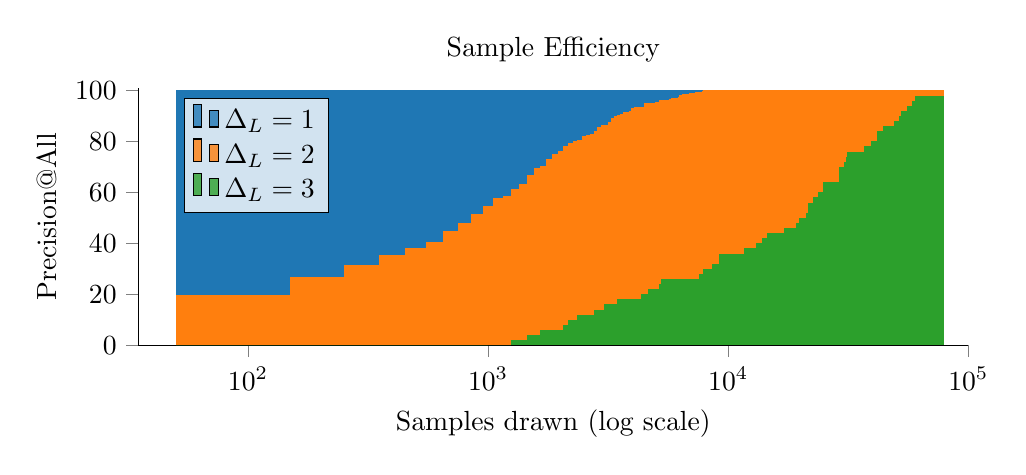
\begin{tikzpicture}

\definecolor{darkgray176}{RGB}{176,176,176}
\definecolor{darkorange25512714}{RGB}{255,127,14}
\definecolor{forestgreen4416044}{RGB}{44,160,44}
\definecolor{steelblue31119180}{RGB}{31,119,180}

\begin{axis}[
width=\textwidth,
height=.4\textwidth,
log basis x={10},
tick align=outside,
tick pos=left,
axis lines*=left,
title={Sample Efficiency},
legend style={fill opacity=0.8, draw opacity=1, text opacity=1, legend columns=1, legend pos=north west, at={(0.055, 0.96)}},
x grid style={darkgray176},
xlabel={Samples drawn (log scale)},
xmin=0.34892211545542, xmax=1001,
xmode=log,
%xtick style={color=black},
xtick={0.01,0.1,1,10,100,1000,10000},
xticklabels={
  \(\displaystyle 10^-2\),
  \(\displaystyle 10^-1\),
  \(\displaystyle 10^2\),
  \(\displaystyle 10^3\),
  \(\displaystyle 10^4\),
  \(\displaystyle 10^5\),
  \(\displaystyle 10^6\)
},
y grid style={darkgray176},
ylabel={Precision@All},
ymin=0, ymax=101,
%ytick style={color=black}
ytick={0,20,40,60,80,100}
]
\draw[draw=none,fill=steelblue31119180] (axis cs:-0.5,0) rectangle (axis cs:0.5,100);
\addlegendimage{ybar,ybar legend,draw=none,fill=steelblue31119180}
\addlegendentry{$\Delta_L=1$}

\draw[draw=none,fill=steelblue31119180] (axis cs:0.5,0) rectangle (axis cs:1.5,100);
\draw[draw=none,fill=steelblue31119180] (axis cs:1.5,0) rectangle (axis cs:2.5,100);
\draw[draw=none,fill=steelblue31119180] (axis cs:2.5,0) rectangle (axis cs:3.5,100);
\draw[draw=none,fill=steelblue31119180] (axis cs:3.5,0) rectangle (axis cs:4.5,100);
\draw[draw=none,fill=steelblue31119180] (axis cs:4.5,0) rectangle (axis cs:5.5,100);
\draw[draw=none,fill=steelblue31119180] (axis cs:5.5,0) rectangle (axis cs:6.5,100);
\draw[draw=none,fill=steelblue31119180] (axis cs:6.5,0) rectangle (axis cs:7.5,100);
\draw[draw=none,fill=steelblue31119180] (axis cs:7.5,0) rectangle (axis cs:8.5,100);
\draw[draw=none,fill=steelblue31119180] (axis cs:8.5,0) rectangle (axis cs:9.5,100);
\draw[draw=none,fill=steelblue31119180] (axis cs:9.5,0) rectangle (axis cs:10.5,100);
\draw[draw=none,fill=steelblue31119180] (axis cs:10.5,0) rectangle (axis cs:11.5,100);
\draw[draw=none,fill=steelblue31119180] (axis cs:11.5,0) rectangle (axis cs:12.5,100);
\draw[draw=none,fill=steelblue31119180] (axis cs:12.5,0) rectangle (axis cs:13.5,100);
\draw[draw=none,fill=steelblue31119180] (axis cs:13.5,0) rectangle (axis cs:14.5,100);
\draw[draw=none,fill=steelblue31119180] (axis cs:14.5,0) rectangle (axis cs:15.5,100);
\draw[draw=none,fill=steelblue31119180] (axis cs:15.5,0) rectangle (axis cs:16.5,100);
\draw[draw=none,fill=steelblue31119180] (axis cs:16.5,0) rectangle (axis cs:17.5,100);
\draw[draw=none,fill=steelblue31119180] (axis cs:17.5,0) rectangle (axis cs:18.5,100);
\draw[draw=none,fill=steelblue31119180] (axis cs:18.5,0) rectangle (axis cs:19.5,100);
\draw[draw=none,fill=steelblue31119180] (axis cs:19.5,0) rectangle (axis cs:20.5,100);
\draw[draw=none,fill=steelblue31119180] (axis cs:20.5,0) rectangle (axis cs:21.5,100);
\draw[draw=none,fill=steelblue31119180] (axis cs:21.5,0) rectangle (axis cs:22.5,100);
\draw[draw=none,fill=steelblue31119180] (axis cs:22.5,0) rectangle (axis cs:23.5,100);
\draw[draw=none,fill=steelblue31119180] (axis cs:23.5,0) rectangle (axis cs:24.5,100);
\draw[draw=none,fill=steelblue31119180] (axis cs:24.5,0) rectangle (axis cs:25.5,100);
\draw[draw=none,fill=steelblue31119180] (axis cs:25.5,0) rectangle (axis cs:26.5,100);
\draw[draw=none,fill=steelblue31119180] (axis cs:26.5,0) rectangle (axis cs:27.5,100);
\draw[draw=none,fill=steelblue31119180] (axis cs:27.5,0) rectangle (axis cs:28.5,100);
\draw[draw=none,fill=steelblue31119180] (axis cs:28.5,0) rectangle (axis cs:29.5,100);
\draw[draw=none,fill=steelblue31119180] (axis cs:29.5,0) rectangle (axis cs:30.5,100);
\draw[draw=none,fill=steelblue31119180] (axis cs:30.5,0) rectangle (axis cs:31.5,100);
\draw[draw=none,fill=steelblue31119180] (axis cs:31.5,0) rectangle (axis cs:32.5,100);
\draw[draw=none,fill=steelblue31119180] (axis cs:32.5,0) rectangle (axis cs:33.5,100);
\draw[draw=none,fill=steelblue31119180] (axis cs:33.5,0) rectangle (axis cs:34.5,100);
\draw[draw=none,fill=steelblue31119180] (axis cs:34.5,0) rectangle (axis cs:35.5,100);
\draw[draw=none,fill=steelblue31119180] (axis cs:35.5,0) rectangle (axis cs:36.5,100);
\draw[draw=none,fill=steelblue31119180] (axis cs:36.5,0) rectangle (axis cs:37.5,100);
\draw[draw=none,fill=steelblue31119180] (axis cs:37.5,0) rectangle (axis cs:38.5,100);
\draw[draw=none,fill=steelblue31119180] (axis cs:38.5,0) rectangle (axis cs:39.5,100);
\draw[draw=none,fill=steelblue31119180] (axis cs:39.5,0) rectangle (axis cs:40.5,100);
\draw[draw=none,fill=steelblue31119180] (axis cs:40.5,0) rectangle (axis cs:41.5,100);
\draw[draw=none,fill=steelblue31119180] (axis cs:41.5,0) rectangle (axis cs:42.5,100);
\draw[draw=none,fill=steelblue31119180] (axis cs:42.5,0) rectangle (axis cs:43.5,100);
\draw[draw=none,fill=steelblue31119180] (axis cs:43.5,0) rectangle (axis cs:44.5,100);
\draw[draw=none,fill=steelblue31119180] (axis cs:44.5,0) rectangle (axis cs:45.5,100);
\draw[draw=none,fill=steelblue31119180] (axis cs:45.5,0) rectangle (axis cs:46.5,100);
\draw[draw=none,fill=steelblue31119180] (axis cs:46.5,0) rectangle (axis cs:47.5,100);
\draw[draw=none,fill=steelblue31119180] (axis cs:47.5,0) rectangle (axis cs:48.5,100);
\draw[draw=none,fill=steelblue31119180] (axis cs:48.5,0) rectangle (axis cs:49.5,100);
\draw[draw=none,fill=steelblue31119180] (axis cs:49.5,0) rectangle (axis cs:50.5,100);
\draw[draw=none,fill=steelblue31119180] (axis cs:50.5,0) rectangle (axis cs:51.5,100);
\draw[draw=none,fill=steelblue31119180] (axis cs:51.5,0) rectangle (axis cs:52.5,100);
\draw[draw=none,fill=steelblue31119180] (axis cs:52.5,0) rectangle (axis cs:53.5,100);
\draw[draw=none,fill=steelblue31119180] (axis cs:53.5,0) rectangle (axis cs:54.5,100);
\draw[draw=none,fill=steelblue31119180] (axis cs:54.5,0) rectangle (axis cs:55.5,100);
\draw[draw=none,fill=steelblue31119180] (axis cs:55.5,0) rectangle (axis cs:56.5,100);
\draw[draw=none,fill=steelblue31119180] (axis cs:56.5,0) rectangle (axis cs:57.5,100);
\draw[draw=none,fill=steelblue31119180] (axis cs:57.5,0) rectangle (axis cs:58.5,100);
\draw[draw=none,fill=steelblue31119180] (axis cs:58.5,0) rectangle (axis cs:59.5,100);
\draw[draw=none,fill=steelblue31119180] (axis cs:59.5,0) rectangle (axis cs:60.5,100);
\draw[draw=none,fill=steelblue31119180] (axis cs:60.5,0) rectangle (axis cs:61.5,100);
\draw[draw=none,fill=steelblue31119180] (axis cs:61.5,0) rectangle (axis cs:62.5,100);
\draw[draw=none,fill=steelblue31119180] (axis cs:62.5,0) rectangle (axis cs:63.5,100);
\draw[draw=none,fill=steelblue31119180] (axis cs:63.5,0) rectangle (axis cs:64.5,100);
\draw[draw=none,fill=steelblue31119180] (axis cs:64.5,0) rectangle (axis cs:65.5,100);
\draw[draw=none,fill=steelblue31119180] (axis cs:65.5,0) rectangle (axis cs:66.5,100);
\draw[draw=none,fill=steelblue31119180] (axis cs:66.5,0) rectangle (axis cs:67.5,100);
\draw[draw=none,fill=steelblue31119180] (axis cs:67.5,0) rectangle (axis cs:68.5,100);
\draw[draw=none,fill=steelblue31119180] (axis cs:68.5,0) rectangle (axis cs:69.5,100);
\draw[draw=none,fill=steelblue31119180] (axis cs:69.5,0) rectangle (axis cs:70.5,100);
\draw[draw=none,fill=steelblue31119180] (axis cs:70.5,0) rectangle (axis cs:71.5,100);
\draw[draw=none,fill=steelblue31119180] (axis cs:71.5,0) rectangle (axis cs:72.5,100);
\draw[draw=none,fill=steelblue31119180] (axis cs:72.5,0) rectangle (axis cs:73.5,100);
\draw[draw=none,fill=steelblue31119180] (axis cs:73.5,0) rectangle (axis cs:74.5,100);
\draw[draw=none,fill=steelblue31119180] (axis cs:74.5,0) rectangle (axis cs:75.5,100);
\draw[draw=none,fill=steelblue31119180] (axis cs:75.5,0) rectangle (axis cs:76.5,100);
\draw[draw=none,fill=steelblue31119180] (axis cs:76.5,0) rectangle (axis cs:77.5,100);
\draw[draw=none,fill=steelblue31119180] (axis cs:77.5,0) rectangle (axis cs:78.5,100);
\draw[draw=none,fill=steelblue31119180] (axis cs:78.5,0) rectangle (axis cs:79.5,100);
\draw[draw=none,fill=steelblue31119180] (axis cs:79.5,0) rectangle (axis cs:80.5,100);
\draw[draw=none,fill=steelblue31119180] (axis cs:80.5,0) rectangle (axis cs:81.5,100);
\draw[draw=none,fill=steelblue31119180] (axis cs:81.5,0) rectangle (axis cs:82.5,100);
\draw[draw=none,fill=steelblue31119180] (axis cs:82.5,0) rectangle (axis cs:83.5,100);
\draw[draw=none,fill=steelblue31119180] (axis cs:83.5,0) rectangle (axis cs:84.5,100);
\draw[draw=none,fill=steelblue31119180] (axis cs:84.5,0) rectangle (axis cs:85.5,100);
\draw[draw=none,fill=steelblue31119180] (axis cs:85.5,0) rectangle (axis cs:86.5,100);
\draw[draw=none,fill=steelblue31119180] (axis cs:86.5,0) rectangle (axis cs:87.5,100);
\draw[draw=none,fill=steelblue31119180] (axis cs:87.5,0) rectangle (axis cs:88.5,100);
\draw[draw=none,fill=steelblue31119180] (axis cs:88.5,0) rectangle (axis cs:89.5,100);
\draw[draw=none,fill=steelblue31119180] (axis cs:89.5,0) rectangle (axis cs:90.5,100);
\draw[draw=none,fill=steelblue31119180] (axis cs:90.5,0) rectangle (axis cs:91.5,100);
\draw[draw=none,fill=steelblue31119180] (axis cs:91.5,0) rectangle (axis cs:92.5,100);
\draw[draw=none,fill=steelblue31119180] (axis cs:92.5,0) rectangle (axis cs:93.5,100);
\draw[draw=none,fill=steelblue31119180] (axis cs:93.5,0) rectangle (axis cs:94.5,100);
\draw[draw=none,fill=steelblue31119180] (axis cs:94.5,0) rectangle (axis cs:95.5,100);
\draw[draw=none,fill=steelblue31119180] (axis cs:95.5,0) rectangle (axis cs:96.5,100);
\draw[draw=none,fill=steelblue31119180] (axis cs:96.5,0) rectangle (axis cs:97.5,100);
\draw[draw=none,fill=steelblue31119180] (axis cs:97.5,0) rectangle (axis cs:98.5,100);
\draw[draw=none,fill=steelblue31119180] (axis cs:98.5,0) rectangle (axis cs:99.5,100);
\draw[draw=none,fill=steelblue31119180] (axis cs:99.5,0) rectangle (axis cs:100.5,100);
\draw[draw=none,fill=steelblue31119180] (axis cs:100.5,0) rectangle (axis cs:101.5,100);
\draw[draw=none,fill=steelblue31119180] (axis cs:101.5,0) rectangle (axis cs:102.5,100);
\draw[draw=none,fill=steelblue31119180] (axis cs:102.5,0) rectangle (axis cs:103.5,100);
\draw[draw=none,fill=steelblue31119180] (axis cs:103.5,0) rectangle (axis cs:104.5,100);
\draw[draw=none,fill=steelblue31119180] (axis cs:104.5,0) rectangle (axis cs:105.5,100);
\draw[draw=none,fill=steelblue31119180] (axis cs:105.5,0) rectangle (axis cs:106.5,100);
\draw[draw=none,fill=steelblue31119180] (axis cs:106.5,0) rectangle (axis cs:107.5,100);
\draw[draw=none,fill=steelblue31119180] (axis cs:107.5,0) rectangle (axis cs:108.5,100);
\draw[draw=none,fill=steelblue31119180] (axis cs:108.5,0) rectangle (axis cs:109.5,100);
\draw[draw=none,fill=steelblue31119180] (axis cs:109.5,0) rectangle (axis cs:110.5,100);
\draw[draw=none,fill=steelblue31119180] (axis cs:110.5,0) rectangle (axis cs:111.5,100);
\draw[draw=none,fill=steelblue31119180] (axis cs:111.5,0) rectangle (axis cs:112.5,100);
\draw[draw=none,fill=steelblue31119180] (axis cs:112.5,0) rectangle (axis cs:113.5,100);
\draw[draw=none,fill=steelblue31119180] (axis cs:113.5,0) rectangle (axis cs:114.5,100);
\draw[draw=none,fill=steelblue31119180] (axis cs:114.5,0) rectangle (axis cs:115.5,100);
\draw[draw=none,fill=steelblue31119180] (axis cs:115.5,0) rectangle (axis cs:116.5,100);
\draw[draw=none,fill=steelblue31119180] (axis cs:116.5,0) rectangle (axis cs:117.5,100);
\draw[draw=none,fill=steelblue31119180] (axis cs:117.5,0) rectangle (axis cs:118.5,100);
\draw[draw=none,fill=steelblue31119180] (axis cs:118.5,0) rectangle (axis cs:119.5,100);
\draw[draw=none,fill=steelblue31119180] (axis cs:119.5,0) rectangle (axis cs:120.5,100);
\draw[draw=none,fill=steelblue31119180] (axis cs:120.5,0) rectangle (axis cs:121.5,100);
\draw[draw=none,fill=steelblue31119180] (axis cs:121.5,0) rectangle (axis cs:122.5,100);
\draw[draw=none,fill=steelblue31119180] (axis cs:122.5,0) rectangle (axis cs:123.5,100);
\draw[draw=none,fill=steelblue31119180] (axis cs:123.5,0) rectangle (axis cs:124.5,100);
\draw[draw=none,fill=steelblue31119180] (axis cs:124.5,0) rectangle (axis cs:125.5,100);
\draw[draw=none,fill=steelblue31119180] (axis cs:125.5,0) rectangle (axis cs:126.5,100);
\draw[draw=none,fill=steelblue31119180] (axis cs:126.5,0) rectangle (axis cs:127.5,100);
\draw[draw=none,fill=steelblue31119180] (axis cs:127.5,0) rectangle (axis cs:128.5,100);
\draw[draw=none,fill=steelblue31119180] (axis cs:128.5,0) rectangle (axis cs:129.5,100);
\draw[draw=none,fill=steelblue31119180] (axis cs:129.5,0) rectangle (axis cs:130.5,100);
\draw[draw=none,fill=steelblue31119180] (axis cs:130.5,0) rectangle (axis cs:131.5,100);
\draw[draw=none,fill=steelblue31119180] (axis cs:131.5,0) rectangle (axis cs:132.5,100);
\draw[draw=none,fill=steelblue31119180] (axis cs:132.5,0) rectangle (axis cs:133.5,100);
\draw[draw=none,fill=steelblue31119180] (axis cs:133.5,0) rectangle (axis cs:134.5,100);
\draw[draw=none,fill=steelblue31119180] (axis cs:134.5,0) rectangle (axis cs:135.5,100);
\draw[draw=none,fill=steelblue31119180] (axis cs:135.5,0) rectangle (axis cs:136.5,100);
\draw[draw=none,fill=steelblue31119180] (axis cs:136.5,0) rectangle (axis cs:137.5,100);
\draw[draw=none,fill=steelblue31119180] (axis cs:137.5,0) rectangle (axis cs:138.5,100);
\draw[draw=none,fill=steelblue31119180] (axis cs:138.5,0) rectangle (axis cs:139.5,100);
\draw[draw=none,fill=steelblue31119180] (axis cs:139.5,0) rectangle (axis cs:140.5,100);
\draw[draw=none,fill=steelblue31119180] (axis cs:140.5,0) rectangle (axis cs:141.5,100);
\draw[draw=none,fill=steelblue31119180] (axis cs:141.5,0) rectangle (axis cs:142.5,100);
\draw[draw=none,fill=steelblue31119180] (axis cs:142.5,0) rectangle (axis cs:143.5,100);
\draw[draw=none,fill=steelblue31119180] (axis cs:143.5,0) rectangle (axis cs:144.5,100);
\draw[draw=none,fill=steelblue31119180] (axis cs:144.5,0) rectangle (axis cs:145.5,100);
\draw[draw=none,fill=steelblue31119180] (axis cs:145.5,0) rectangle (axis cs:146.5,100);
\draw[draw=none,fill=steelblue31119180] (axis cs:146.5,0) rectangle (axis cs:147.5,100);
\draw[draw=none,fill=steelblue31119180] (axis cs:147.5,0) rectangle (axis cs:148.5,100);
\draw[draw=none,fill=steelblue31119180] (axis cs:148.5,0) rectangle (axis cs:149.5,100);
\draw[draw=none,fill=steelblue31119180] (axis cs:149.5,0) rectangle (axis cs:150.5,100);
\draw[draw=none,fill=steelblue31119180] (axis cs:150.5,0) rectangle (axis cs:151.5,100);
\draw[draw=none,fill=steelblue31119180] (axis cs:151.5,0) rectangle (axis cs:152.5,100);
\draw[draw=none,fill=steelblue31119180] (axis cs:152.5,0) rectangle (axis cs:153.5,100);
\draw[draw=none,fill=steelblue31119180] (axis cs:153.5,0) rectangle (axis cs:154.5,100);
\draw[draw=none,fill=steelblue31119180] (axis cs:154.5,0) rectangle (axis cs:155.5,100);
\draw[draw=none,fill=steelblue31119180] (axis cs:155.5,0) rectangle (axis cs:156.5,100);
\draw[draw=none,fill=steelblue31119180] (axis cs:156.5,0) rectangle (axis cs:157.5,100);
\draw[draw=none,fill=steelblue31119180] (axis cs:157.5,0) rectangle (axis cs:158.5,100);
\draw[draw=none,fill=steelblue31119180] (axis cs:158.5,0) rectangle (axis cs:159.5,100);
\draw[draw=none,fill=steelblue31119180] (axis cs:159.5,0) rectangle (axis cs:160.5,100);
\draw[draw=none,fill=steelblue31119180] (axis cs:160.5,0) rectangle (axis cs:161.5,100);
\draw[draw=none,fill=steelblue31119180] (axis cs:161.5,0) rectangle (axis cs:162.5,100);
\draw[draw=none,fill=steelblue31119180] (axis cs:162.5,0) rectangle (axis cs:163.5,100);
\draw[draw=none,fill=steelblue31119180] (axis cs:163.5,0) rectangle (axis cs:164.5,100);
\draw[draw=none,fill=steelblue31119180] (axis cs:164.5,0) rectangle (axis cs:165.5,100);
\draw[draw=none,fill=steelblue31119180] (axis cs:165.5,0) rectangle (axis cs:166.5,100);
\draw[draw=none,fill=steelblue31119180] (axis cs:166.5,0) rectangle (axis cs:167.5,100);
\draw[draw=none,fill=steelblue31119180] (axis cs:167.5,0) rectangle (axis cs:168.5,100);
\draw[draw=none,fill=steelblue31119180] (axis cs:168.5,0) rectangle (axis cs:169.5,100);
\draw[draw=none,fill=steelblue31119180] (axis cs:169.5,0) rectangle (axis cs:170.5,100);
\draw[draw=none,fill=steelblue31119180] (axis cs:170.5,0) rectangle (axis cs:171.5,100);
\draw[draw=none,fill=steelblue31119180] (axis cs:171.5,0) rectangle (axis cs:172.5,100);
\draw[draw=none,fill=steelblue31119180] (axis cs:172.5,0) rectangle (axis cs:173.5,100);
\draw[draw=none,fill=steelblue31119180] (axis cs:173.5,0) rectangle (axis cs:174.5,100);
\draw[draw=none,fill=steelblue31119180] (axis cs:174.5,0) rectangle (axis cs:175.5,100);
\draw[draw=none,fill=steelblue31119180] (axis cs:175.5,0) rectangle (axis cs:176.5,100);
\draw[draw=none,fill=steelblue31119180] (axis cs:176.5,0) rectangle (axis cs:177.5,100);
\draw[draw=none,fill=steelblue31119180] (axis cs:177.5,0) rectangle (axis cs:178.5,100);
\draw[draw=none,fill=steelblue31119180] (axis cs:178.5,0) rectangle (axis cs:179.5,100);
\draw[draw=none,fill=steelblue31119180] (axis cs:179.5,0) rectangle (axis cs:180.5,100);
\draw[draw=none,fill=steelblue31119180] (axis cs:180.5,0) rectangle (axis cs:181.5,100);
\draw[draw=none,fill=steelblue31119180] (axis cs:181.5,0) rectangle (axis cs:182.5,100);
\draw[draw=none,fill=steelblue31119180] (axis cs:182.5,0) rectangle (axis cs:183.5,100);
\draw[draw=none,fill=steelblue31119180] (axis cs:183.5,0) rectangle (axis cs:184.5,100);
\draw[draw=none,fill=steelblue31119180] (axis cs:184.5,0) rectangle (axis cs:185.5,100);
\draw[draw=none,fill=steelblue31119180] (axis cs:185.5,0) rectangle (axis cs:186.5,100);
\draw[draw=none,fill=steelblue31119180] (axis cs:186.5,0) rectangle (axis cs:187.5,100);
\draw[draw=none,fill=steelblue31119180] (axis cs:187.5,0) rectangle (axis cs:188.5,100);
\draw[draw=none,fill=steelblue31119180] (axis cs:188.5,0) rectangle (axis cs:189.5,100);
\draw[draw=none,fill=steelblue31119180] (axis cs:189.5,0) rectangle (axis cs:190.5,100);
\draw[draw=none,fill=steelblue31119180] (axis cs:190.5,0) rectangle (axis cs:191.5,100);
\draw[draw=none,fill=steelblue31119180] (axis cs:191.5,0) rectangle (axis cs:192.5,100);
\draw[draw=none,fill=steelblue31119180] (axis cs:192.5,0) rectangle (axis cs:193.5,100);
\draw[draw=none,fill=steelblue31119180] (axis cs:193.5,0) rectangle (axis cs:194.5,100);
\draw[draw=none,fill=steelblue31119180] (axis cs:194.5,0) rectangle (axis cs:195.5,100);
\draw[draw=none,fill=steelblue31119180] (axis cs:195.5,0) rectangle (axis cs:196.5,100);
\draw[draw=none,fill=steelblue31119180] (axis cs:196.5,0) rectangle (axis cs:197.5,100);
\draw[draw=none,fill=steelblue31119180] (axis cs:197.5,0) rectangle (axis cs:198.5,100);
\draw[draw=none,fill=steelblue31119180] (axis cs:198.5,0) rectangle (axis cs:199.5,100);
\draw[draw=none,fill=steelblue31119180] (axis cs:199.5,0) rectangle (axis cs:200.5,100);
\draw[draw=none,fill=steelblue31119180] (axis cs:200.5,0) rectangle (axis cs:201.5,100);
\draw[draw=none,fill=steelblue31119180] (axis cs:201.5,0) rectangle (axis cs:202.5,100);
\draw[draw=none,fill=steelblue31119180] (axis cs:202.5,0) rectangle (axis cs:203.5,100);
\draw[draw=none,fill=steelblue31119180] (axis cs:203.5,0) rectangle (axis cs:204.5,100);
\draw[draw=none,fill=steelblue31119180] (axis cs:204.5,0) rectangle (axis cs:205.5,100);
\draw[draw=none,fill=steelblue31119180] (axis cs:205.5,0) rectangle (axis cs:206.5,100);
\draw[draw=none,fill=steelblue31119180] (axis cs:206.5,0) rectangle (axis cs:207.5,100);
\draw[draw=none,fill=steelblue31119180] (axis cs:207.5,0) rectangle (axis cs:208.5,100);
\draw[draw=none,fill=steelblue31119180] (axis cs:208.5,0) rectangle (axis cs:209.5,100);
\draw[draw=none,fill=steelblue31119180] (axis cs:209.5,0) rectangle (axis cs:210.5,100);
\draw[draw=none,fill=steelblue31119180] (axis cs:210.5,0) rectangle (axis cs:211.5,100);
\draw[draw=none,fill=steelblue31119180] (axis cs:211.5,0) rectangle (axis cs:212.5,100);
\draw[draw=none,fill=steelblue31119180] (axis cs:212.5,0) rectangle (axis cs:213.5,100);
\draw[draw=none,fill=steelblue31119180] (axis cs:213.5,0) rectangle (axis cs:214.5,100);
\draw[draw=none,fill=steelblue31119180] (axis cs:214.5,0) rectangle (axis cs:215.5,100);
\draw[draw=none,fill=steelblue31119180] (axis cs:215.5,0) rectangle (axis cs:216.5,100);
\draw[draw=none,fill=steelblue31119180] (axis cs:216.5,0) rectangle (axis cs:217.5,100);
\draw[draw=none,fill=steelblue31119180] (axis cs:217.5,0) rectangle (axis cs:218.5,100);
\draw[draw=none,fill=steelblue31119180] (axis cs:218.5,0) rectangle (axis cs:219.5,100);
\draw[draw=none,fill=steelblue31119180] (axis cs:219.5,0) rectangle (axis cs:220.5,100);
\draw[draw=none,fill=steelblue31119180] (axis cs:220.5,0) rectangle (axis cs:221.5,100);
\draw[draw=none,fill=steelblue31119180] (axis cs:221.5,0) rectangle (axis cs:222.5,100);
\draw[draw=none,fill=steelblue31119180] (axis cs:222.5,0) rectangle (axis cs:223.5,100);
\draw[draw=none,fill=steelblue31119180] (axis cs:223.5,0) rectangle (axis cs:224.5,100);
\draw[draw=none,fill=steelblue31119180] (axis cs:224.5,0) rectangle (axis cs:225.5,100);
\draw[draw=none,fill=steelblue31119180] (axis cs:225.5,0) rectangle (axis cs:226.5,100);
\draw[draw=none,fill=steelblue31119180] (axis cs:226.5,0) rectangle (axis cs:227.5,100);
\draw[draw=none,fill=steelblue31119180] (axis cs:227.5,0) rectangle (axis cs:228.5,100);
\draw[draw=none,fill=steelblue31119180] (axis cs:228.5,0) rectangle (axis cs:229.5,100);
\draw[draw=none,fill=steelblue31119180] (axis cs:229.5,0) rectangle (axis cs:230.5,100);
\draw[draw=none,fill=steelblue31119180] (axis cs:230.5,0) rectangle (axis cs:231.5,100);
\draw[draw=none,fill=steelblue31119180] (axis cs:231.5,0) rectangle (axis cs:232.5,100);
\draw[draw=none,fill=steelblue31119180] (axis cs:232.5,0) rectangle (axis cs:233.5,100);
\draw[draw=none,fill=steelblue31119180] (axis cs:233.5,0) rectangle (axis cs:234.5,100);
\draw[draw=none,fill=steelblue31119180] (axis cs:234.5,0) rectangle (axis cs:235.5,100);
\draw[draw=none,fill=steelblue31119180] (axis cs:235.5,0) rectangle (axis cs:236.5,100);
\draw[draw=none,fill=steelblue31119180] (axis cs:236.5,0) rectangle (axis cs:237.5,100);
\draw[draw=none,fill=steelblue31119180] (axis cs:237.5,0) rectangle (axis cs:238.5,100);
\draw[draw=none,fill=steelblue31119180] (axis cs:238.5,0) rectangle (axis cs:239.5,100);
\draw[draw=none,fill=steelblue31119180] (axis cs:239.5,0) rectangle (axis cs:240.5,100);
\draw[draw=none,fill=steelblue31119180] (axis cs:240.5,0) rectangle (axis cs:241.5,100);
\draw[draw=none,fill=steelblue31119180] (axis cs:241.5,0) rectangle (axis cs:242.5,100);
\draw[draw=none,fill=steelblue31119180] (axis cs:242.5,0) rectangle (axis cs:243.5,100);
\draw[draw=none,fill=steelblue31119180] (axis cs:243.5,0) rectangle (axis cs:244.5,100);
\draw[draw=none,fill=steelblue31119180] (axis cs:244.5,0) rectangle (axis cs:245.5,100);
\draw[draw=none,fill=steelblue31119180] (axis cs:245.5,0) rectangle (axis cs:246.5,100);
\draw[draw=none,fill=steelblue31119180] (axis cs:246.5,0) rectangle (axis cs:247.5,100);
\draw[draw=none,fill=steelblue31119180] (axis cs:247.5,0) rectangle (axis cs:248.5,100);
\draw[draw=none,fill=steelblue31119180] (axis cs:248.5,0) rectangle (axis cs:249.5,100);
\draw[draw=none,fill=steelblue31119180] (axis cs:249.5,0) rectangle (axis cs:250.5,100);
\draw[draw=none,fill=steelblue31119180] (axis cs:250.5,0) rectangle (axis cs:251.5,100);
\draw[draw=none,fill=steelblue31119180] (axis cs:251.5,0) rectangle (axis cs:252.5,100);
\draw[draw=none,fill=steelblue31119180] (axis cs:252.5,0) rectangle (axis cs:253.5,100);
\draw[draw=none,fill=steelblue31119180] (axis cs:253.5,0) rectangle (axis cs:254.5,100);
\draw[draw=none,fill=steelblue31119180] (axis cs:254.5,0) rectangle (axis cs:255.5,100);
\draw[draw=none,fill=steelblue31119180] (axis cs:255.5,0) rectangle (axis cs:256.5,100);
\draw[draw=none,fill=steelblue31119180] (axis cs:256.5,0) rectangle (axis cs:257.5,100);
\draw[draw=none,fill=steelblue31119180] (axis cs:257.5,0) rectangle (axis cs:258.5,100);
\draw[draw=none,fill=steelblue31119180] (axis cs:258.5,0) rectangle (axis cs:259.5,100);
\draw[draw=none,fill=steelblue31119180] (axis cs:259.5,0) rectangle (axis cs:260.5,100);
\draw[draw=none,fill=steelblue31119180] (axis cs:260.5,0) rectangle (axis cs:261.5,100);
\draw[draw=none,fill=steelblue31119180] (axis cs:261.5,0) rectangle (axis cs:262.5,100);
\draw[draw=none,fill=steelblue31119180] (axis cs:262.5,0) rectangle (axis cs:263.5,100);
\draw[draw=none,fill=steelblue31119180] (axis cs:263.5,0) rectangle (axis cs:264.5,100);
\draw[draw=none,fill=steelblue31119180] (axis cs:264.5,0) rectangle (axis cs:265.5,100);
\draw[draw=none,fill=steelblue31119180] (axis cs:265.5,0) rectangle (axis cs:266.5,100);
\draw[draw=none,fill=steelblue31119180] (axis cs:266.5,0) rectangle (axis cs:267.5,100);
\draw[draw=none,fill=steelblue31119180] (axis cs:267.5,0) rectangle (axis cs:268.5,100);
\draw[draw=none,fill=steelblue31119180] (axis cs:268.5,0) rectangle (axis cs:269.5,100);
\draw[draw=none,fill=steelblue31119180] (axis cs:269.5,0) rectangle (axis cs:270.5,100);
\draw[draw=none,fill=steelblue31119180] (axis cs:270.5,0) rectangle (axis cs:271.5,100);
\draw[draw=none,fill=steelblue31119180] (axis cs:271.5,0) rectangle (axis cs:272.5,100);
\draw[draw=none,fill=steelblue31119180] (axis cs:272.5,0) rectangle (axis cs:273.5,100);
\draw[draw=none,fill=steelblue31119180] (axis cs:273.5,0) rectangle (axis cs:274.5,100);
\draw[draw=none,fill=steelblue31119180] (axis cs:274.5,0) rectangle (axis cs:275.5,100);
\draw[draw=none,fill=steelblue31119180] (axis cs:275.5,0) rectangle (axis cs:276.5,100);
\draw[draw=none,fill=steelblue31119180] (axis cs:276.5,0) rectangle (axis cs:277.5,100);
\draw[draw=none,fill=steelblue31119180] (axis cs:277.5,0) rectangle (axis cs:278.5,100);
\draw[draw=none,fill=steelblue31119180] (axis cs:278.5,0) rectangle (axis cs:279.5,100);
\draw[draw=none,fill=steelblue31119180] (axis cs:279.5,0) rectangle (axis cs:280.5,100);
\draw[draw=none,fill=steelblue31119180] (axis cs:280.5,0) rectangle (axis cs:281.5,100);
\draw[draw=none,fill=steelblue31119180] (axis cs:281.5,0) rectangle (axis cs:282.5,100);
\draw[draw=none,fill=steelblue31119180] (axis cs:282.5,0) rectangle (axis cs:283.5,100);
\draw[draw=none,fill=steelblue31119180] (axis cs:283.5,0) rectangle (axis cs:284.5,100);
\draw[draw=none,fill=steelblue31119180] (axis cs:284.5,0) rectangle (axis cs:285.5,100);
\draw[draw=none,fill=steelblue31119180] (axis cs:285.5,0) rectangle (axis cs:286.5,100);
\draw[draw=none,fill=steelblue31119180] (axis cs:286.5,0) rectangle (axis cs:287.5,100);
\draw[draw=none,fill=steelblue31119180] (axis cs:287.5,0) rectangle (axis cs:288.5,100);
\draw[draw=none,fill=steelblue31119180] (axis cs:288.5,0) rectangle (axis cs:289.5,100);
\draw[draw=none,fill=steelblue31119180] (axis cs:289.5,0) rectangle (axis cs:290.5,100);
\draw[draw=none,fill=steelblue31119180] (axis cs:290.5,0) rectangle (axis cs:291.5,100);
\draw[draw=none,fill=steelblue31119180] (axis cs:291.5,0) rectangle (axis cs:292.5,100);
\draw[draw=none,fill=steelblue31119180] (axis cs:292.5,0) rectangle (axis cs:293.5,100);
\draw[draw=none,fill=steelblue31119180] (axis cs:293.5,0) rectangle (axis cs:294.5,100);
\draw[draw=none,fill=steelblue31119180] (axis cs:294.5,0) rectangle (axis cs:295.5,100);
\draw[draw=none,fill=steelblue31119180] (axis cs:295.5,0) rectangle (axis cs:296.5,100);
\draw[draw=none,fill=steelblue31119180] (axis cs:296.5,0) rectangle (axis cs:297.5,100);
\draw[draw=none,fill=steelblue31119180] (axis cs:297.5,0) rectangle (axis cs:298.5,100);
\draw[draw=none,fill=steelblue31119180] (axis cs:298.5,0) rectangle (axis cs:299.5,100);
\draw[draw=none,fill=steelblue31119180] (axis cs:299.5,0) rectangle (axis cs:300.5,100);
\draw[draw=none,fill=steelblue31119180] (axis cs:300.5,0) rectangle (axis cs:301.5,100);
\draw[draw=none,fill=steelblue31119180] (axis cs:301.5,0) rectangle (axis cs:302.5,100);
\draw[draw=none,fill=steelblue31119180] (axis cs:302.5,0) rectangle (axis cs:303.5,100);
\draw[draw=none,fill=steelblue31119180] (axis cs:303.5,0) rectangle (axis cs:304.5,100);
\draw[draw=none,fill=steelblue31119180] (axis cs:304.5,0) rectangle (axis cs:305.5,100);
\draw[draw=none,fill=steelblue31119180] (axis cs:305.5,0) rectangle (axis cs:306.5,100);
\draw[draw=none,fill=steelblue31119180] (axis cs:306.5,0) rectangle (axis cs:307.5,100);
\draw[draw=none,fill=steelblue31119180] (axis cs:307.5,0) rectangle (axis cs:308.5,100);
\draw[draw=none,fill=steelblue31119180] (axis cs:308.5,0) rectangle (axis cs:309.5,100);
\draw[draw=none,fill=steelblue31119180] (axis cs:309.5,0) rectangle (axis cs:310.5,100);
\draw[draw=none,fill=steelblue31119180] (axis cs:310.5,0) rectangle (axis cs:311.5,100);
\draw[draw=none,fill=steelblue31119180] (axis cs:311.5,0) rectangle (axis cs:312.5,100);
\draw[draw=none,fill=steelblue31119180] (axis cs:312.5,0) rectangle (axis cs:313.5,100);
\draw[draw=none,fill=steelblue31119180] (axis cs:313.5,0) rectangle (axis cs:314.5,100);
\draw[draw=none,fill=steelblue31119180] (axis cs:314.5,0) rectangle (axis cs:315.5,100);
\draw[draw=none,fill=steelblue31119180] (axis cs:315.5,0) rectangle (axis cs:316.5,100);
\draw[draw=none,fill=steelblue31119180] (axis cs:316.5,0) rectangle (axis cs:317.5,100);
\draw[draw=none,fill=steelblue31119180] (axis cs:317.5,0) rectangle (axis cs:318.5,100);
\draw[draw=none,fill=steelblue31119180] (axis cs:318.5,0) rectangle (axis cs:319.5,100);
\draw[draw=none,fill=steelblue31119180] (axis cs:319.5,0) rectangle (axis cs:320.5,100);
\draw[draw=none,fill=steelblue31119180] (axis cs:320.5,0) rectangle (axis cs:321.5,100);
\draw[draw=none,fill=steelblue31119180] (axis cs:321.5,0) rectangle (axis cs:322.5,100);
\draw[draw=none,fill=steelblue31119180] (axis cs:322.5,0) rectangle (axis cs:323.5,100);
\draw[draw=none,fill=steelblue31119180] (axis cs:323.5,0) rectangle (axis cs:324.5,100);
\draw[draw=none,fill=steelblue31119180] (axis cs:324.5,0) rectangle (axis cs:325.5,100);
\draw[draw=none,fill=steelblue31119180] (axis cs:325.5,0) rectangle (axis cs:326.5,100);
\draw[draw=none,fill=steelblue31119180] (axis cs:326.5,0) rectangle (axis cs:327.5,100);
\draw[draw=none,fill=steelblue31119180] (axis cs:327.5,0) rectangle (axis cs:328.5,100);
\draw[draw=none,fill=steelblue31119180] (axis cs:328.5,0) rectangle (axis cs:329.5,100);
\draw[draw=none,fill=steelblue31119180] (axis cs:329.5,0) rectangle (axis cs:330.5,100);
\draw[draw=none,fill=steelblue31119180] (axis cs:330.5,0) rectangle (axis cs:331.5,100);
\draw[draw=none,fill=steelblue31119180] (axis cs:331.5,0) rectangle (axis cs:332.5,100);
\draw[draw=none,fill=steelblue31119180] (axis cs:332.5,0) rectangle (axis cs:333.5,100);
\draw[draw=none,fill=steelblue31119180] (axis cs:333.5,0) rectangle (axis cs:334.5,100);
\draw[draw=none,fill=steelblue31119180] (axis cs:334.5,0) rectangle (axis cs:335.5,100);
\draw[draw=none,fill=steelblue31119180] (axis cs:335.5,0) rectangle (axis cs:336.5,100);
\draw[draw=none,fill=steelblue31119180] (axis cs:336.5,0) rectangle (axis cs:337.5,100);
\draw[draw=none,fill=steelblue31119180] (axis cs:337.5,0) rectangle (axis cs:338.5,100);
\draw[draw=none,fill=steelblue31119180] (axis cs:338.5,0) rectangle (axis cs:339.5,100);
\draw[draw=none,fill=steelblue31119180] (axis cs:339.5,0) rectangle (axis cs:340.5,100);
\draw[draw=none,fill=steelblue31119180] (axis cs:340.5,0) rectangle (axis cs:341.5,100);
\draw[draw=none,fill=steelblue31119180] (axis cs:341.5,0) rectangle (axis cs:342.5,100);
\draw[draw=none,fill=steelblue31119180] (axis cs:342.5,0) rectangle (axis cs:343.5,100);
\draw[draw=none,fill=steelblue31119180] (axis cs:343.5,0) rectangle (axis cs:344.5,100);
\draw[draw=none,fill=steelblue31119180] (axis cs:344.5,0) rectangle (axis cs:345.5,100);
\draw[draw=none,fill=steelblue31119180] (axis cs:345.5,0) rectangle (axis cs:346.5,100);
\draw[draw=none,fill=steelblue31119180] (axis cs:346.5,0) rectangle (axis cs:347.5,100);
\draw[draw=none,fill=steelblue31119180] (axis cs:347.5,0) rectangle (axis cs:348.5,100);
\draw[draw=none,fill=steelblue31119180] (axis cs:348.5,0) rectangle (axis cs:349.5,100);
\draw[draw=none,fill=steelblue31119180] (axis cs:349.5,0) rectangle (axis cs:350.5,100);
\draw[draw=none,fill=steelblue31119180] (axis cs:350.5,0) rectangle (axis cs:351.5,100);
\draw[draw=none,fill=steelblue31119180] (axis cs:351.5,0) rectangle (axis cs:352.5,100);
\draw[draw=none,fill=steelblue31119180] (axis cs:352.5,0) rectangle (axis cs:353.5,100);
\draw[draw=none,fill=steelblue31119180] (axis cs:353.5,0) rectangle (axis cs:354.5,100);
\draw[draw=none,fill=steelblue31119180] (axis cs:354.5,0) rectangle (axis cs:355.5,100);
\draw[draw=none,fill=steelblue31119180] (axis cs:355.5,0) rectangle (axis cs:356.5,100);
\draw[draw=none,fill=steelblue31119180] (axis cs:356.5,0) rectangle (axis cs:357.5,100);
\draw[draw=none,fill=steelblue31119180] (axis cs:357.5,0) rectangle (axis cs:358.5,100);
\draw[draw=none,fill=steelblue31119180] (axis cs:358.5,0) rectangle (axis cs:359.5,100);
\draw[draw=none,fill=steelblue31119180] (axis cs:359.5,0) rectangle (axis cs:360.5,100);
\draw[draw=none,fill=steelblue31119180] (axis cs:360.5,0) rectangle (axis cs:361.5,100);
\draw[draw=none,fill=steelblue31119180] (axis cs:361.5,0) rectangle (axis cs:362.5,100);
\draw[draw=none,fill=steelblue31119180] (axis cs:362.5,0) rectangle (axis cs:363.5,100);
\draw[draw=none,fill=steelblue31119180] (axis cs:363.5,0) rectangle (axis cs:364.5,100);
\draw[draw=none,fill=steelblue31119180] (axis cs:364.5,0) rectangle (axis cs:365.5,100);
\draw[draw=none,fill=steelblue31119180] (axis cs:365.5,0) rectangle (axis cs:366.5,100);
\draw[draw=none,fill=steelblue31119180] (axis cs:366.5,0) rectangle (axis cs:367.5,100);
\draw[draw=none,fill=steelblue31119180] (axis cs:367.5,0) rectangle (axis cs:368.5,100);
\draw[draw=none,fill=steelblue31119180] (axis cs:368.5,0) rectangle (axis cs:369.5,100);
\draw[draw=none,fill=steelblue31119180] (axis cs:369.5,0) rectangle (axis cs:370.5,100);
\draw[draw=none,fill=steelblue31119180] (axis cs:370.5,0) rectangle (axis cs:371.5,100);
\draw[draw=none,fill=steelblue31119180] (axis cs:371.5,0) rectangle (axis cs:372.5,100);
\draw[draw=none,fill=steelblue31119180] (axis cs:372.5,0) rectangle (axis cs:373.5,100);
\draw[draw=none,fill=steelblue31119180] (axis cs:373.5,0) rectangle (axis cs:374.5,100);
\draw[draw=none,fill=steelblue31119180] (axis cs:374.5,0) rectangle (axis cs:375.5,100);
\draw[draw=none,fill=steelblue31119180] (axis cs:375.5,0) rectangle (axis cs:376.5,100);
\draw[draw=none,fill=steelblue31119180] (axis cs:376.5,0) rectangle (axis cs:377.5,100);
\draw[draw=none,fill=steelblue31119180] (axis cs:377.5,0) rectangle (axis cs:378.5,100);
\draw[draw=none,fill=steelblue31119180] (axis cs:378.5,0) rectangle (axis cs:379.5,100);
\draw[draw=none,fill=steelblue31119180] (axis cs:379.5,0) rectangle (axis cs:380.5,100);
\draw[draw=none,fill=steelblue31119180] (axis cs:380.5,0) rectangle (axis cs:381.5,100);
\draw[draw=none,fill=steelblue31119180] (axis cs:381.5,0) rectangle (axis cs:382.5,100);
\draw[draw=none,fill=steelblue31119180] (axis cs:382.5,0) rectangle (axis cs:383.5,100);
\draw[draw=none,fill=steelblue31119180] (axis cs:383.5,0) rectangle (axis cs:384.5,100);
\draw[draw=none,fill=steelblue31119180] (axis cs:384.5,0) rectangle (axis cs:385.5,100);
\draw[draw=none,fill=steelblue31119180] (axis cs:385.5,0) rectangle (axis cs:386.5,100);
\draw[draw=none,fill=steelblue31119180] (axis cs:386.5,0) rectangle (axis cs:387.5,100);
\draw[draw=none,fill=steelblue31119180] (axis cs:387.5,0) rectangle (axis cs:388.5,100);
\draw[draw=none,fill=steelblue31119180] (axis cs:388.5,0) rectangle (axis cs:389.5,100);
\draw[draw=none,fill=steelblue31119180] (axis cs:389.5,0) rectangle (axis cs:390.5,100);
\draw[draw=none,fill=steelblue31119180] (axis cs:390.5,0) rectangle (axis cs:391.5,100);
\draw[draw=none,fill=steelblue31119180] (axis cs:391.5,0) rectangle (axis cs:392.5,100);
\draw[draw=none,fill=steelblue31119180] (axis cs:392.5,0) rectangle (axis cs:393.5,100);
\draw[draw=none,fill=steelblue31119180] (axis cs:393.5,0) rectangle (axis cs:394.5,100);
\draw[draw=none,fill=steelblue31119180] (axis cs:394.5,0) rectangle (axis cs:395.5,100);
\draw[draw=none,fill=steelblue31119180] (axis cs:395.5,0) rectangle (axis cs:396.5,100);
\draw[draw=none,fill=steelblue31119180] (axis cs:396.5,0) rectangle (axis cs:397.5,100);
\draw[draw=none,fill=steelblue31119180] (axis cs:397.5,0) rectangle (axis cs:398.5,100);
\draw[draw=none,fill=steelblue31119180] (axis cs:398.5,0) rectangle (axis cs:399.5,100);
\draw[draw=none,fill=steelblue31119180] (axis cs:399.5,0) rectangle (axis cs:400.5,100);
\draw[draw=none,fill=steelblue31119180] (axis cs:400.5,0) rectangle (axis cs:401.5,100);
\draw[draw=none,fill=steelblue31119180] (axis cs:401.5,0) rectangle (axis cs:402.5,100);
\draw[draw=none,fill=steelblue31119180] (axis cs:402.5,0) rectangle (axis cs:403.5,100);
\draw[draw=none,fill=steelblue31119180] (axis cs:403.5,0) rectangle (axis cs:404.5,100);
\draw[draw=none,fill=steelblue31119180] (axis cs:404.5,0) rectangle (axis cs:405.5,100);
\draw[draw=none,fill=steelblue31119180] (axis cs:405.5,0) rectangle (axis cs:406.5,100);
\draw[draw=none,fill=steelblue31119180] (axis cs:406.5,0) rectangle (axis cs:407.5,100);
\draw[draw=none,fill=steelblue31119180] (axis cs:407.5,0) rectangle (axis cs:408.5,100);
\draw[draw=none,fill=steelblue31119180] (axis cs:408.5,0) rectangle (axis cs:409.5,100);
\draw[draw=none,fill=steelblue31119180] (axis cs:409.5,0) rectangle (axis cs:410.5,100);
\draw[draw=none,fill=steelblue31119180] (axis cs:410.5,0) rectangle (axis cs:411.5,100);
\draw[draw=none,fill=steelblue31119180] (axis cs:411.5,0) rectangle (axis cs:412.5,100);
\draw[draw=none,fill=steelblue31119180] (axis cs:412.5,0) rectangle (axis cs:413.5,100);
\draw[draw=none,fill=steelblue31119180] (axis cs:413.5,0) rectangle (axis cs:414.5,100);
\draw[draw=none,fill=steelblue31119180] (axis cs:414.5,0) rectangle (axis cs:415.5,100);
\draw[draw=none,fill=steelblue31119180] (axis cs:415.5,0) rectangle (axis cs:416.5,100);
\draw[draw=none,fill=steelblue31119180] (axis cs:416.5,0) rectangle (axis cs:417.5,100);
\draw[draw=none,fill=steelblue31119180] (axis cs:417.5,0) rectangle (axis cs:418.5,100);
\draw[draw=none,fill=steelblue31119180] (axis cs:418.5,0) rectangle (axis cs:419.5,100);
\draw[draw=none,fill=steelblue31119180] (axis cs:419.5,0) rectangle (axis cs:420.5,100);
\draw[draw=none,fill=steelblue31119180] (axis cs:420.5,0) rectangle (axis cs:421.5,100);
\draw[draw=none,fill=steelblue31119180] (axis cs:421.5,0) rectangle (axis cs:422.5,100);
\draw[draw=none,fill=steelblue31119180] (axis cs:422.5,0) rectangle (axis cs:423.5,100);
\draw[draw=none,fill=steelblue31119180] (axis cs:423.5,0) rectangle (axis cs:424.5,100);
\draw[draw=none,fill=steelblue31119180] (axis cs:424.5,0) rectangle (axis cs:425.5,100);
\draw[draw=none,fill=steelblue31119180] (axis cs:425.5,0) rectangle (axis cs:426.5,100);
\draw[draw=none,fill=steelblue31119180] (axis cs:426.5,0) rectangle (axis cs:427.5,100);
\draw[draw=none,fill=steelblue31119180] (axis cs:427.5,0) rectangle (axis cs:428.5,100);
\draw[draw=none,fill=steelblue31119180] (axis cs:428.5,0) rectangle (axis cs:429.5,100);
\draw[draw=none,fill=steelblue31119180] (axis cs:429.5,0) rectangle (axis cs:430.5,100);
\draw[draw=none,fill=steelblue31119180] (axis cs:430.5,0) rectangle (axis cs:431.5,100);
\draw[draw=none,fill=steelblue31119180] (axis cs:431.5,0) rectangle (axis cs:432.5,100);
\draw[draw=none,fill=steelblue31119180] (axis cs:432.5,0) rectangle (axis cs:433.5,100);
\draw[draw=none,fill=steelblue31119180] (axis cs:433.5,0) rectangle (axis cs:434.5,100);
\draw[draw=none,fill=steelblue31119180] (axis cs:434.5,0) rectangle (axis cs:435.5,100);
\draw[draw=none,fill=steelblue31119180] (axis cs:435.5,0) rectangle (axis cs:436.5,100);
\draw[draw=none,fill=steelblue31119180] (axis cs:436.5,0) rectangle (axis cs:437.5,100);
\draw[draw=none,fill=steelblue31119180] (axis cs:437.5,0) rectangle (axis cs:438.5,100);
\draw[draw=none,fill=steelblue31119180] (axis cs:438.5,0) rectangle (axis cs:439.5,100);
\draw[draw=none,fill=steelblue31119180] (axis cs:439.5,0) rectangle (axis cs:440.5,100);
\draw[draw=none,fill=steelblue31119180] (axis cs:440.5,0) rectangle (axis cs:441.5,100);
\draw[draw=none,fill=steelblue31119180] (axis cs:441.5,0) rectangle (axis cs:442.5,100);
\draw[draw=none,fill=steelblue31119180] (axis cs:442.5,0) rectangle (axis cs:443.5,100);
\draw[draw=none,fill=steelblue31119180] (axis cs:443.5,0) rectangle (axis cs:444.5,100);
\draw[draw=none,fill=steelblue31119180] (axis cs:444.5,0) rectangle (axis cs:445.5,100);
\draw[draw=none,fill=steelblue31119180] (axis cs:445.5,0) rectangle (axis cs:446.5,100);
\draw[draw=none,fill=steelblue31119180] (axis cs:446.5,0) rectangle (axis cs:447.5,100);
\draw[draw=none,fill=steelblue31119180] (axis cs:447.5,0) rectangle (axis cs:448.5,100);
\draw[draw=none,fill=steelblue31119180] (axis cs:448.5,0) rectangle (axis cs:449.5,100);
\draw[draw=none,fill=steelblue31119180] (axis cs:449.5,0) rectangle (axis cs:450.5,100);
\draw[draw=none,fill=steelblue31119180] (axis cs:450.5,0) rectangle (axis cs:451.5,100);
\draw[draw=none,fill=steelblue31119180] (axis cs:451.5,0) rectangle (axis cs:452.5,100);
\draw[draw=none,fill=steelblue31119180] (axis cs:452.5,0) rectangle (axis cs:453.5,100);
\draw[draw=none,fill=steelblue31119180] (axis cs:453.5,0) rectangle (axis cs:454.5,100);
\draw[draw=none,fill=steelblue31119180] (axis cs:454.5,0) rectangle (axis cs:455.5,100);
\draw[draw=none,fill=steelblue31119180] (axis cs:455.5,0) rectangle (axis cs:456.5,100);
\draw[draw=none,fill=steelblue31119180] (axis cs:456.5,0) rectangle (axis cs:457.5,100);
\draw[draw=none,fill=steelblue31119180] (axis cs:457.5,0) rectangle (axis cs:458.5,100);
\draw[draw=none,fill=steelblue31119180] (axis cs:458.5,0) rectangle (axis cs:459.5,100);
\draw[draw=none,fill=steelblue31119180] (axis cs:459.5,0) rectangle (axis cs:460.5,100);
\draw[draw=none,fill=steelblue31119180] (axis cs:460.5,0) rectangle (axis cs:461.5,100);
\draw[draw=none,fill=steelblue31119180] (axis cs:461.5,0) rectangle (axis cs:462.5,100);
\draw[draw=none,fill=steelblue31119180] (axis cs:462.5,0) rectangle (axis cs:463.5,100);
\draw[draw=none,fill=steelblue31119180] (axis cs:463.5,0) rectangle (axis cs:464.5,100);
\draw[draw=none,fill=steelblue31119180] (axis cs:464.5,0) rectangle (axis cs:465.5,100);
\draw[draw=none,fill=steelblue31119180] (axis cs:465.5,0) rectangle (axis cs:466.5,100);
\draw[draw=none,fill=steelblue31119180] (axis cs:466.5,0) rectangle (axis cs:467.5,100);
\draw[draw=none,fill=steelblue31119180] (axis cs:467.5,0) rectangle (axis cs:468.5,100);
\draw[draw=none,fill=steelblue31119180] (axis cs:468.5,0) rectangle (axis cs:469.5,100);
\draw[draw=none,fill=steelblue31119180] (axis cs:469.5,0) rectangle (axis cs:470.5,100);
\draw[draw=none,fill=steelblue31119180] (axis cs:470.5,0) rectangle (axis cs:471.5,100);
\draw[draw=none,fill=steelblue31119180] (axis cs:471.5,0) rectangle (axis cs:472.5,100);
\draw[draw=none,fill=steelblue31119180] (axis cs:472.5,0) rectangle (axis cs:473.5,100);
\draw[draw=none,fill=steelblue31119180] (axis cs:473.5,0) rectangle (axis cs:474.5,100);
\draw[draw=none,fill=steelblue31119180] (axis cs:474.5,0) rectangle (axis cs:475.5,100);
\draw[draw=none,fill=steelblue31119180] (axis cs:475.5,0) rectangle (axis cs:476.5,100);
\draw[draw=none,fill=steelblue31119180] (axis cs:476.5,0) rectangle (axis cs:477.5,100);
\draw[draw=none,fill=steelblue31119180] (axis cs:477.5,0) rectangle (axis cs:478.5,100);
\draw[draw=none,fill=steelblue31119180] (axis cs:478.5,0) rectangle (axis cs:479.5,100);
\draw[draw=none,fill=steelblue31119180] (axis cs:479.5,0) rectangle (axis cs:480.5,100);
\draw[draw=none,fill=steelblue31119180] (axis cs:480.5,0) rectangle (axis cs:481.5,100);
\draw[draw=none,fill=steelblue31119180] (axis cs:481.5,0) rectangle (axis cs:482.5,100);
\draw[draw=none,fill=steelblue31119180] (axis cs:482.5,0) rectangle (axis cs:483.5,100);
\draw[draw=none,fill=steelblue31119180] (axis cs:483.5,0) rectangle (axis cs:484.5,100);
\draw[draw=none,fill=steelblue31119180] (axis cs:484.5,0) rectangle (axis cs:485.5,100);
\draw[draw=none,fill=steelblue31119180] (axis cs:485.5,0) rectangle (axis cs:486.5,100);
\draw[draw=none,fill=steelblue31119180] (axis cs:486.5,0) rectangle (axis cs:487.5,100);
\draw[draw=none,fill=steelblue31119180] (axis cs:487.5,0) rectangle (axis cs:488.5,100);
\draw[draw=none,fill=steelblue31119180] (axis cs:488.5,0) rectangle (axis cs:489.5,100);
\draw[draw=none,fill=steelblue31119180] (axis cs:489.5,0) rectangle (axis cs:490.5,100);
\draw[draw=none,fill=steelblue31119180] (axis cs:490.5,0) rectangle (axis cs:491.5,100);
\draw[draw=none,fill=steelblue31119180] (axis cs:491.5,0) rectangle (axis cs:492.5,100);
\draw[draw=none,fill=steelblue31119180] (axis cs:492.5,0) rectangle (axis cs:493.5,100);
\draw[draw=none,fill=steelblue31119180] (axis cs:493.5,0) rectangle (axis cs:494.5,100);
\draw[draw=none,fill=steelblue31119180] (axis cs:494.5,0) rectangle (axis cs:495.5,100);
\draw[draw=none,fill=steelblue31119180] (axis cs:495.5,0) rectangle (axis cs:496.5,100);
\draw[draw=none,fill=steelblue31119180] (axis cs:496.5,0) rectangle (axis cs:497.5,100);
\draw[draw=none,fill=steelblue31119180] (axis cs:497.5,0) rectangle (axis cs:498.5,100);
\draw[draw=none,fill=steelblue31119180] (axis cs:498.5,0) rectangle (axis cs:499.5,100);
\draw[draw=none,fill=steelblue31119180] (axis cs:499.5,0) rectangle (axis cs:500.5,100);
\draw[draw=none,fill=steelblue31119180] (axis cs:500.5,0) rectangle (axis cs:501.5,100);
\draw[draw=none,fill=steelblue31119180] (axis cs:501.5,0) rectangle (axis cs:502.5,100);
\draw[draw=none,fill=steelblue31119180] (axis cs:502.5,0) rectangle (axis cs:503.5,100);
\draw[draw=none,fill=steelblue31119180] (axis cs:503.5,0) rectangle (axis cs:504.5,100);
\draw[draw=none,fill=steelblue31119180] (axis cs:504.5,0) rectangle (axis cs:505.5,100);
\draw[draw=none,fill=steelblue31119180] (axis cs:505.5,0) rectangle (axis cs:506.5,100);
\draw[draw=none,fill=steelblue31119180] (axis cs:506.5,0) rectangle (axis cs:507.5,100);
\draw[draw=none,fill=steelblue31119180] (axis cs:507.5,0) rectangle (axis cs:508.5,100);
\draw[draw=none,fill=steelblue31119180] (axis cs:508.5,0) rectangle (axis cs:509.5,100);
\draw[draw=none,fill=steelblue31119180] (axis cs:509.5,0) rectangle (axis cs:510.5,100);
\draw[draw=none,fill=steelblue31119180] (axis cs:510.5,0) rectangle (axis cs:511.5,100);
\draw[draw=none,fill=steelblue31119180] (axis cs:511.5,0) rectangle (axis cs:512.5,100);
\draw[draw=none,fill=steelblue31119180] (axis cs:512.5,0) rectangle (axis cs:513.5,100);
\draw[draw=none,fill=steelblue31119180] (axis cs:513.5,0) rectangle (axis cs:514.5,100);
\draw[draw=none,fill=steelblue31119180] (axis cs:514.5,0) rectangle (axis cs:515.5,100);
\draw[draw=none,fill=steelblue31119180] (axis cs:515.5,0) rectangle (axis cs:516.5,100);
\draw[draw=none,fill=steelblue31119180] (axis cs:516.5,0) rectangle (axis cs:517.5,100);
\draw[draw=none,fill=steelblue31119180] (axis cs:517.5,0) rectangle (axis cs:518.5,100);
\draw[draw=none,fill=steelblue31119180] (axis cs:518.5,0) rectangle (axis cs:519.5,100);
\draw[draw=none,fill=steelblue31119180] (axis cs:519.5,0) rectangle (axis cs:520.5,100);
\draw[draw=none,fill=steelblue31119180] (axis cs:520.5,0) rectangle (axis cs:521.5,100);
\draw[draw=none,fill=steelblue31119180] (axis cs:521.5,0) rectangle (axis cs:522.5,100);
\draw[draw=none,fill=steelblue31119180] (axis cs:522.5,0) rectangle (axis cs:523.5,100);
\draw[draw=none,fill=steelblue31119180] (axis cs:523.5,0) rectangle (axis cs:524.5,100);
\draw[draw=none,fill=steelblue31119180] (axis cs:524.5,0) rectangle (axis cs:525.5,100);
\draw[draw=none,fill=steelblue31119180] (axis cs:525.5,0) rectangle (axis cs:526.5,100);
\draw[draw=none,fill=steelblue31119180] (axis cs:526.5,0) rectangle (axis cs:527.5,100);
\draw[draw=none,fill=steelblue31119180] (axis cs:527.5,0) rectangle (axis cs:528.5,100);
\draw[draw=none,fill=steelblue31119180] (axis cs:528.5,0) rectangle (axis cs:529.5,100);
\draw[draw=none,fill=steelblue31119180] (axis cs:529.5,0) rectangle (axis cs:530.5,100);
\draw[draw=none,fill=steelblue31119180] (axis cs:530.5,0) rectangle (axis cs:531.5,100);
\draw[draw=none,fill=steelblue31119180] (axis cs:531.5,0) rectangle (axis cs:532.5,100);
\draw[draw=none,fill=steelblue31119180] (axis cs:532.5,0) rectangle (axis cs:533.5,100);
\draw[draw=none,fill=steelblue31119180] (axis cs:533.5,0) rectangle (axis cs:534.5,100);
\draw[draw=none,fill=steelblue31119180] (axis cs:534.5,0) rectangle (axis cs:535.5,100);
\draw[draw=none,fill=steelblue31119180] (axis cs:535.5,0) rectangle (axis cs:536.5,100);
\draw[draw=none,fill=steelblue31119180] (axis cs:536.5,0) rectangle (axis cs:537.5,100);
\draw[draw=none,fill=steelblue31119180] (axis cs:537.5,0) rectangle (axis cs:538.5,100);
\draw[draw=none,fill=steelblue31119180] (axis cs:538.5,0) rectangle (axis cs:539.5,100);
\draw[draw=none,fill=steelblue31119180] (axis cs:539.5,0) rectangle (axis cs:540.5,100);
\draw[draw=none,fill=steelblue31119180] (axis cs:540.5,0) rectangle (axis cs:541.5,100);
\draw[draw=none,fill=steelblue31119180] (axis cs:541.5,0) rectangle (axis cs:542.5,100);
\draw[draw=none,fill=steelblue31119180] (axis cs:542.5,0) rectangle (axis cs:543.5,100);
\draw[draw=none,fill=steelblue31119180] (axis cs:543.5,0) rectangle (axis cs:544.5,100);
\draw[draw=none,fill=steelblue31119180] (axis cs:544.5,0) rectangle (axis cs:545.5,100);
\draw[draw=none,fill=steelblue31119180] (axis cs:545.5,0) rectangle (axis cs:546.5,100);
\draw[draw=none,fill=steelblue31119180] (axis cs:546.5,0) rectangle (axis cs:547.5,100);
\draw[draw=none,fill=steelblue31119180] (axis cs:547.5,0) rectangle (axis cs:548.5,100);
\draw[draw=none,fill=steelblue31119180] (axis cs:548.5,0) rectangle (axis cs:549.5,100);
\draw[draw=none,fill=steelblue31119180] (axis cs:549.5,0) rectangle (axis cs:550.5,100);
\draw[draw=none,fill=steelblue31119180] (axis cs:550.5,0) rectangle (axis cs:551.5,100);
\draw[draw=none,fill=steelblue31119180] (axis cs:551.5,0) rectangle (axis cs:552.5,100);
\draw[draw=none,fill=steelblue31119180] (axis cs:552.5,0) rectangle (axis cs:553.5,100);
\draw[draw=none,fill=steelblue31119180] (axis cs:553.5,0) rectangle (axis cs:554.5,100);
\draw[draw=none,fill=steelblue31119180] (axis cs:554.5,0) rectangle (axis cs:555.5,100);
\draw[draw=none,fill=steelblue31119180] (axis cs:555.5,0) rectangle (axis cs:556.5,100);
\draw[draw=none,fill=steelblue31119180] (axis cs:556.5,0) rectangle (axis cs:557.5,100);
\draw[draw=none,fill=steelblue31119180] (axis cs:557.5,0) rectangle (axis cs:558.5,100);
\draw[draw=none,fill=steelblue31119180] (axis cs:558.5,0) rectangle (axis cs:559.5,100);
\draw[draw=none,fill=steelblue31119180] (axis cs:559.5,0) rectangle (axis cs:560.5,100);
\draw[draw=none,fill=steelblue31119180] (axis cs:560.5,0) rectangle (axis cs:561.5,100);
\draw[draw=none,fill=steelblue31119180] (axis cs:561.5,0) rectangle (axis cs:562.5,100);
\draw[draw=none,fill=steelblue31119180] (axis cs:562.5,0) rectangle (axis cs:563.5,100);
\draw[draw=none,fill=steelblue31119180] (axis cs:563.5,0) rectangle (axis cs:564.5,100);
\draw[draw=none,fill=steelblue31119180] (axis cs:564.5,0) rectangle (axis cs:565.5,100);
\draw[draw=none,fill=steelblue31119180] (axis cs:565.5,0) rectangle (axis cs:566.5,100);
\draw[draw=none,fill=steelblue31119180] (axis cs:566.5,0) rectangle (axis cs:567.5,100);
\draw[draw=none,fill=steelblue31119180] (axis cs:567.5,0) rectangle (axis cs:568.5,100);
\draw[draw=none,fill=steelblue31119180] (axis cs:568.5,0) rectangle (axis cs:569.5,100);
\draw[draw=none,fill=steelblue31119180] (axis cs:569.5,0) rectangle (axis cs:570.5,100);
\draw[draw=none,fill=steelblue31119180] (axis cs:570.5,0) rectangle (axis cs:571.5,100);
\draw[draw=none,fill=steelblue31119180] (axis cs:571.5,0) rectangle (axis cs:572.5,100);
\draw[draw=none,fill=steelblue31119180] (axis cs:572.5,0) rectangle (axis cs:573.5,100);
\draw[draw=none,fill=steelblue31119180] (axis cs:573.5,0) rectangle (axis cs:574.5,100);
\draw[draw=none,fill=steelblue31119180] (axis cs:574.5,0) rectangle (axis cs:575.5,100);
\draw[draw=none,fill=steelblue31119180] (axis cs:575.5,0) rectangle (axis cs:576.5,100);
\draw[draw=none,fill=steelblue31119180] (axis cs:576.5,0) rectangle (axis cs:577.5,100);
\draw[draw=none,fill=steelblue31119180] (axis cs:577.5,0) rectangle (axis cs:578.5,100);
\draw[draw=none,fill=steelblue31119180] (axis cs:578.5,0) rectangle (axis cs:579.5,100);
\draw[draw=none,fill=steelblue31119180] (axis cs:579.5,0) rectangle (axis cs:580.5,100);
\draw[draw=none,fill=steelblue31119180] (axis cs:580.5,0) rectangle (axis cs:581.5,100);
\draw[draw=none,fill=steelblue31119180] (axis cs:581.5,0) rectangle (axis cs:582.5,100);
\draw[draw=none,fill=steelblue31119180] (axis cs:582.5,0) rectangle (axis cs:583.5,100);
\draw[draw=none,fill=steelblue31119180] (axis cs:583.5,0) rectangle (axis cs:584.5,100);
\draw[draw=none,fill=steelblue31119180] (axis cs:584.5,0) rectangle (axis cs:585.5,100);
\draw[draw=none,fill=steelblue31119180] (axis cs:585.5,0) rectangle (axis cs:586.5,100);
\draw[draw=none,fill=steelblue31119180] (axis cs:586.5,0) rectangle (axis cs:587.5,100);
\draw[draw=none,fill=steelblue31119180] (axis cs:587.5,0) rectangle (axis cs:588.5,100);
\draw[draw=none,fill=steelblue31119180] (axis cs:588.5,0) rectangle (axis cs:589.5,100);
\draw[draw=none,fill=steelblue31119180] (axis cs:589.5,0) rectangle (axis cs:590.5,100);
\draw[draw=none,fill=steelblue31119180] (axis cs:590.5,0) rectangle (axis cs:591.5,100);
\draw[draw=none,fill=steelblue31119180] (axis cs:591.5,0) rectangle (axis cs:592.5,100);
\draw[draw=none,fill=steelblue31119180] (axis cs:592.5,0) rectangle (axis cs:593.5,100);
\draw[draw=none,fill=steelblue31119180] (axis cs:593.5,0) rectangle (axis cs:594.5,100);
\draw[draw=none,fill=steelblue31119180] (axis cs:594.5,0) rectangle (axis cs:595.5,100);
\draw[draw=none,fill=steelblue31119180] (axis cs:595.5,0) rectangle (axis cs:596.5,100);
\draw[draw=none,fill=steelblue31119180] (axis cs:596.5,0) rectangle (axis cs:597.5,100);
\draw[draw=none,fill=steelblue31119180] (axis cs:597.5,0) rectangle (axis cs:598.5,100);
\draw[draw=none,fill=steelblue31119180] (axis cs:598.5,0) rectangle (axis cs:599.5,100);
\draw[draw=none,fill=steelblue31119180] (axis cs:599.5,0) rectangle (axis cs:600.5,100);
\draw[draw=none,fill=steelblue31119180] (axis cs:600.5,0) rectangle (axis cs:601.5,100);
\draw[draw=none,fill=steelblue31119180] (axis cs:601.5,0) rectangle (axis cs:602.5,100);
\draw[draw=none,fill=steelblue31119180] (axis cs:602.5,0) rectangle (axis cs:603.5,100);
\draw[draw=none,fill=steelblue31119180] (axis cs:603.5,0) rectangle (axis cs:604.5,100);
\draw[draw=none,fill=steelblue31119180] (axis cs:604.5,0) rectangle (axis cs:605.5,100);
\draw[draw=none,fill=steelblue31119180] (axis cs:605.5,0) rectangle (axis cs:606.5,100);
\draw[draw=none,fill=steelblue31119180] (axis cs:606.5,0) rectangle (axis cs:607.5,100);
\draw[draw=none,fill=steelblue31119180] (axis cs:607.5,0) rectangle (axis cs:608.5,100);
\draw[draw=none,fill=steelblue31119180] (axis cs:608.5,0) rectangle (axis cs:609.5,100);
\draw[draw=none,fill=steelblue31119180] (axis cs:609.5,0) rectangle (axis cs:610.5,100);
\draw[draw=none,fill=steelblue31119180] (axis cs:610.5,0) rectangle (axis cs:611.5,100);
\draw[draw=none,fill=steelblue31119180] (axis cs:611.5,0) rectangle (axis cs:612.5,100);
\draw[draw=none,fill=steelblue31119180] (axis cs:612.5,0) rectangle (axis cs:613.5,100);
\draw[draw=none,fill=steelblue31119180] (axis cs:613.5,0) rectangle (axis cs:614.5,100);
\draw[draw=none,fill=steelblue31119180] (axis cs:614.5,0) rectangle (axis cs:615.5,100);
\draw[draw=none,fill=steelblue31119180] (axis cs:615.5,0) rectangle (axis cs:616.5,100);
\draw[draw=none,fill=steelblue31119180] (axis cs:616.5,0) rectangle (axis cs:617.5,100);
\draw[draw=none,fill=steelblue31119180] (axis cs:617.5,0) rectangle (axis cs:618.5,100);
\draw[draw=none,fill=steelblue31119180] (axis cs:618.5,0) rectangle (axis cs:619.5,100);
\draw[draw=none,fill=steelblue31119180] (axis cs:619.5,0) rectangle (axis cs:620.5,100);
\draw[draw=none,fill=steelblue31119180] (axis cs:620.5,0) rectangle (axis cs:621.5,100);
\draw[draw=none,fill=steelblue31119180] (axis cs:621.5,0) rectangle (axis cs:622.5,100);
\draw[draw=none,fill=steelblue31119180] (axis cs:622.5,0) rectangle (axis cs:623.5,100);
\draw[draw=none,fill=steelblue31119180] (axis cs:623.5,0) rectangle (axis cs:624.5,100);
\draw[draw=none,fill=steelblue31119180] (axis cs:624.5,0) rectangle (axis cs:625.5,100);
\draw[draw=none,fill=steelblue31119180] (axis cs:625.5,0) rectangle (axis cs:626.5,100);
\draw[draw=none,fill=steelblue31119180] (axis cs:626.5,0) rectangle (axis cs:627.5,100);
\draw[draw=none,fill=steelblue31119180] (axis cs:627.5,0) rectangle (axis cs:628.5,100);
\draw[draw=none,fill=steelblue31119180] (axis cs:628.5,0) rectangle (axis cs:629.5,100);
\draw[draw=none,fill=steelblue31119180] (axis cs:629.5,0) rectangle (axis cs:630.5,100);
\draw[draw=none,fill=steelblue31119180] (axis cs:630.5,0) rectangle (axis cs:631.5,100);
\draw[draw=none,fill=steelblue31119180] (axis cs:631.5,0) rectangle (axis cs:632.5,100);
\draw[draw=none,fill=steelblue31119180] (axis cs:632.5,0) rectangle (axis cs:633.5,100);
\draw[draw=none,fill=steelblue31119180] (axis cs:633.5,0) rectangle (axis cs:634.5,100);
\draw[draw=none,fill=steelblue31119180] (axis cs:634.5,0) rectangle (axis cs:635.5,100);
\draw[draw=none,fill=steelblue31119180] (axis cs:635.5,0) rectangle (axis cs:636.5,100);
\draw[draw=none,fill=steelblue31119180] (axis cs:636.5,0) rectangle (axis cs:637.5,100);
\draw[draw=none,fill=steelblue31119180] (axis cs:637.5,0) rectangle (axis cs:638.5,100);
\draw[draw=none,fill=steelblue31119180] (axis cs:638.5,0) rectangle (axis cs:639.5,100);
\draw[draw=none,fill=steelblue31119180] (axis cs:639.5,0) rectangle (axis cs:640.5,100);
\draw[draw=none,fill=steelblue31119180] (axis cs:640.5,0) rectangle (axis cs:641.5,100);
\draw[draw=none,fill=steelblue31119180] (axis cs:641.5,0) rectangle (axis cs:642.5,100);
\draw[draw=none,fill=steelblue31119180] (axis cs:642.5,0) rectangle (axis cs:643.5,100);
\draw[draw=none,fill=steelblue31119180] (axis cs:643.5,0) rectangle (axis cs:644.5,100);
\draw[draw=none,fill=steelblue31119180] (axis cs:644.5,0) rectangle (axis cs:645.5,100);
\draw[draw=none,fill=steelblue31119180] (axis cs:645.5,0) rectangle (axis cs:646.5,100);
\draw[draw=none,fill=steelblue31119180] (axis cs:646.5,0) rectangle (axis cs:647.5,100);
\draw[draw=none,fill=steelblue31119180] (axis cs:647.5,0) rectangle (axis cs:648.5,100);
\draw[draw=none,fill=steelblue31119180] (axis cs:648.5,0) rectangle (axis cs:649.5,100);
\draw[draw=none,fill=steelblue31119180] (axis cs:649.5,0) rectangle (axis cs:650.5,100);
\draw[draw=none,fill=steelblue31119180] (axis cs:650.5,0) rectangle (axis cs:651.5,100);
\draw[draw=none,fill=steelblue31119180] (axis cs:651.5,0) rectangle (axis cs:652.5,100);
\draw[draw=none,fill=steelblue31119180] (axis cs:652.5,0) rectangle (axis cs:653.5,100);
\draw[draw=none,fill=steelblue31119180] (axis cs:653.5,0) rectangle (axis cs:654.5,100);
\draw[draw=none,fill=steelblue31119180] (axis cs:654.5,0) rectangle (axis cs:655.5,100);
\draw[draw=none,fill=steelblue31119180] (axis cs:655.5,0) rectangle (axis cs:656.5,100);
\draw[draw=none,fill=steelblue31119180] (axis cs:656.5,0) rectangle (axis cs:657.5,100);
\draw[draw=none,fill=steelblue31119180] (axis cs:657.5,0) rectangle (axis cs:658.5,100);
\draw[draw=none,fill=steelblue31119180] (axis cs:658.5,0) rectangle (axis cs:659.5,100);
\draw[draw=none,fill=steelblue31119180] (axis cs:659.5,0) rectangle (axis cs:660.5,100);
\draw[draw=none,fill=steelblue31119180] (axis cs:660.5,0) rectangle (axis cs:661.5,100);
\draw[draw=none,fill=steelblue31119180] (axis cs:661.5,0) rectangle (axis cs:662.5,100);
\draw[draw=none,fill=steelblue31119180] (axis cs:662.5,0) rectangle (axis cs:663.5,100);
\draw[draw=none,fill=steelblue31119180] (axis cs:663.5,0) rectangle (axis cs:664.5,100);
\draw[draw=none,fill=steelblue31119180] (axis cs:664.5,0) rectangle (axis cs:665.5,100);
\draw[draw=none,fill=steelblue31119180] (axis cs:665.5,0) rectangle (axis cs:666.5,100);
\draw[draw=none,fill=steelblue31119180] (axis cs:666.5,0) rectangle (axis cs:667.5,100);
\draw[draw=none,fill=steelblue31119180] (axis cs:667.5,0) rectangle (axis cs:668.5,100);
\draw[draw=none,fill=steelblue31119180] (axis cs:668.5,0) rectangle (axis cs:669.5,100);
\draw[draw=none,fill=steelblue31119180] (axis cs:669.5,0) rectangle (axis cs:670.5,100);
\draw[draw=none,fill=steelblue31119180] (axis cs:670.5,0) rectangle (axis cs:671.5,100);
\draw[draw=none,fill=steelblue31119180] (axis cs:671.5,0) rectangle (axis cs:672.5,100);
\draw[draw=none,fill=steelblue31119180] (axis cs:672.5,0) rectangle (axis cs:673.5,100);
\draw[draw=none,fill=steelblue31119180] (axis cs:673.5,0) rectangle (axis cs:674.5,100);
\draw[draw=none,fill=steelblue31119180] (axis cs:674.5,0) rectangle (axis cs:675.5,100);
\draw[draw=none,fill=steelblue31119180] (axis cs:675.5,0) rectangle (axis cs:676.5,100);
\draw[draw=none,fill=steelblue31119180] (axis cs:676.5,0) rectangle (axis cs:677.5,100);
\draw[draw=none,fill=steelblue31119180] (axis cs:677.5,0) rectangle (axis cs:678.5,100);
\draw[draw=none,fill=steelblue31119180] (axis cs:678.5,0) rectangle (axis cs:679.5,100);
\draw[draw=none,fill=steelblue31119180] (axis cs:679.5,0) rectangle (axis cs:680.5,100);
\draw[draw=none,fill=steelblue31119180] (axis cs:680.5,0) rectangle (axis cs:681.5,100);
\draw[draw=none,fill=steelblue31119180] (axis cs:681.5,0) rectangle (axis cs:682.5,100);
\draw[draw=none,fill=steelblue31119180] (axis cs:682.5,0) rectangle (axis cs:683.5,100);
\draw[draw=none,fill=steelblue31119180] (axis cs:683.5,0) rectangle (axis cs:684.5,100);
\draw[draw=none,fill=steelblue31119180] (axis cs:684.5,0) rectangle (axis cs:685.5,100);
\draw[draw=none,fill=steelblue31119180] (axis cs:685.5,0) rectangle (axis cs:686.5,100);
\draw[draw=none,fill=steelblue31119180] (axis cs:686.5,0) rectangle (axis cs:687.5,100);
\draw[draw=none,fill=steelblue31119180] (axis cs:687.5,0) rectangle (axis cs:688.5,100);
\draw[draw=none,fill=steelblue31119180] (axis cs:688.5,0) rectangle (axis cs:689.5,100);
\draw[draw=none,fill=steelblue31119180] (axis cs:689.5,0) rectangle (axis cs:690.5,100);
\draw[draw=none,fill=steelblue31119180] (axis cs:690.5,0) rectangle (axis cs:691.5,100);
\draw[draw=none,fill=steelblue31119180] (axis cs:691.5,0) rectangle (axis cs:692.5,100);
\draw[draw=none,fill=steelblue31119180] (axis cs:692.5,0) rectangle (axis cs:693.5,100);
\draw[draw=none,fill=steelblue31119180] (axis cs:693.5,0) rectangle (axis cs:694.5,100);
\draw[draw=none,fill=steelblue31119180] (axis cs:694.5,0) rectangle (axis cs:695.5,100);
\draw[draw=none,fill=steelblue31119180] (axis cs:695.5,0) rectangle (axis cs:696.5,100);
\draw[draw=none,fill=steelblue31119180] (axis cs:696.5,0) rectangle (axis cs:697.5,100);
\draw[draw=none,fill=steelblue31119180] (axis cs:697.5,0) rectangle (axis cs:698.5,100);
\draw[draw=none,fill=steelblue31119180] (axis cs:698.5,0) rectangle (axis cs:699.5,100);
\draw[draw=none,fill=steelblue31119180] (axis cs:699.5,0) rectangle (axis cs:700.5,100);
\draw[draw=none,fill=steelblue31119180] (axis cs:700.5,0) rectangle (axis cs:701.5,100);
\draw[draw=none,fill=steelblue31119180] (axis cs:701.5,0) rectangle (axis cs:702.5,100);
\draw[draw=none,fill=steelblue31119180] (axis cs:702.5,0) rectangle (axis cs:703.5,100);
\draw[draw=none,fill=steelblue31119180] (axis cs:703.5,0) rectangle (axis cs:704.5,100);
\draw[draw=none,fill=steelblue31119180] (axis cs:704.5,0) rectangle (axis cs:705.5,100);
\draw[draw=none,fill=steelblue31119180] (axis cs:705.5,0) rectangle (axis cs:706.5,100);
\draw[draw=none,fill=steelblue31119180] (axis cs:706.5,0) rectangle (axis cs:707.5,100);
\draw[draw=none,fill=steelblue31119180] (axis cs:707.5,0) rectangle (axis cs:708.5,100);
\draw[draw=none,fill=steelblue31119180] (axis cs:708.5,0) rectangle (axis cs:709.5,100);
\draw[draw=none,fill=steelblue31119180] (axis cs:709.5,0) rectangle (axis cs:710.5,100);
\draw[draw=none,fill=steelblue31119180] (axis cs:710.5,0) rectangle (axis cs:711.5,100);
\draw[draw=none,fill=steelblue31119180] (axis cs:711.5,0) rectangle (axis cs:712.5,100);
\draw[draw=none,fill=steelblue31119180] (axis cs:712.5,0) rectangle (axis cs:713.5,100);
\draw[draw=none,fill=steelblue31119180] (axis cs:713.5,0) rectangle (axis cs:714.5,100);
\draw[draw=none,fill=steelblue31119180] (axis cs:714.5,0) rectangle (axis cs:715.5,100);
\draw[draw=none,fill=steelblue31119180] (axis cs:715.5,0) rectangle (axis cs:716.5,100);
\draw[draw=none,fill=steelblue31119180] (axis cs:716.5,0) rectangle (axis cs:717.5,100);
\draw[draw=none,fill=steelblue31119180] (axis cs:717.5,0) rectangle (axis cs:718.5,100);
\draw[draw=none,fill=steelblue31119180] (axis cs:718.5,0) rectangle (axis cs:719.5,100);
\draw[draw=none,fill=steelblue31119180] (axis cs:719.5,0) rectangle (axis cs:720.5,100);
\draw[draw=none,fill=steelblue31119180] (axis cs:720.5,0) rectangle (axis cs:721.5,100);
\draw[draw=none,fill=steelblue31119180] (axis cs:721.5,0) rectangle (axis cs:722.5,100);
\draw[draw=none,fill=steelblue31119180] (axis cs:722.5,0) rectangle (axis cs:723.5,100);
\draw[draw=none,fill=steelblue31119180] (axis cs:723.5,0) rectangle (axis cs:724.5,100);
\draw[draw=none,fill=steelblue31119180] (axis cs:724.5,0) rectangle (axis cs:725.5,100);
\draw[draw=none,fill=steelblue31119180] (axis cs:725.5,0) rectangle (axis cs:726.5,100);
\draw[draw=none,fill=steelblue31119180] (axis cs:726.5,0) rectangle (axis cs:727.5,100);
\draw[draw=none,fill=steelblue31119180] (axis cs:727.5,0) rectangle (axis cs:728.5,100);
\draw[draw=none,fill=steelblue31119180] (axis cs:728.5,0) rectangle (axis cs:729.5,100);
\draw[draw=none,fill=steelblue31119180] (axis cs:729.5,0) rectangle (axis cs:730.5,100);
\draw[draw=none,fill=steelblue31119180] (axis cs:730.5,0) rectangle (axis cs:731.5,100);
\draw[draw=none,fill=steelblue31119180] (axis cs:731.5,0) rectangle (axis cs:732.5,100);
\draw[draw=none,fill=steelblue31119180] (axis cs:732.5,0) rectangle (axis cs:733.5,100);
\draw[draw=none,fill=steelblue31119180] (axis cs:733.5,0) rectangle (axis cs:734.5,100);
\draw[draw=none,fill=steelblue31119180] (axis cs:734.5,0) rectangle (axis cs:735.5,100);
\draw[draw=none,fill=steelblue31119180] (axis cs:735.5,0) rectangle (axis cs:736.5,100);
\draw[draw=none,fill=steelblue31119180] (axis cs:736.5,0) rectangle (axis cs:737.5,100);
\draw[draw=none,fill=steelblue31119180] (axis cs:737.5,0) rectangle (axis cs:738.5,100);
\draw[draw=none,fill=steelblue31119180] (axis cs:738.5,0) rectangle (axis cs:739.5,100);
\draw[draw=none,fill=steelblue31119180] (axis cs:739.5,0) rectangle (axis cs:740.5,100);
\draw[draw=none,fill=steelblue31119180] (axis cs:740.5,0) rectangle (axis cs:741.5,100);
\draw[draw=none,fill=steelblue31119180] (axis cs:741.5,0) rectangle (axis cs:742.5,100);
\draw[draw=none,fill=steelblue31119180] (axis cs:742.5,0) rectangle (axis cs:743.5,100);
\draw[draw=none,fill=steelblue31119180] (axis cs:743.5,0) rectangle (axis cs:744.5,100);
\draw[draw=none,fill=steelblue31119180] (axis cs:744.5,0) rectangle (axis cs:745.5,100);
\draw[draw=none,fill=steelblue31119180] (axis cs:745.5,0) rectangle (axis cs:746.5,100);
\draw[draw=none,fill=steelblue31119180] (axis cs:746.5,0) rectangle (axis cs:747.5,100);
\draw[draw=none,fill=steelblue31119180] (axis cs:747.5,0) rectangle (axis cs:748.5,100);
\draw[draw=none,fill=steelblue31119180] (axis cs:748.5,0) rectangle (axis cs:749.5,100);
\draw[draw=none,fill=steelblue31119180] (axis cs:749.5,0) rectangle (axis cs:750.5,100);
\draw[draw=none,fill=steelblue31119180] (axis cs:750.5,0) rectangle (axis cs:751.5,100);
\draw[draw=none,fill=steelblue31119180] (axis cs:751.5,0) rectangle (axis cs:752.5,100);
\draw[draw=none,fill=steelblue31119180] (axis cs:752.5,0) rectangle (axis cs:753.5,100);
\draw[draw=none,fill=steelblue31119180] (axis cs:753.5,0) rectangle (axis cs:754.5,100);
\draw[draw=none,fill=steelblue31119180] (axis cs:754.5,0) rectangle (axis cs:755.5,100);
\draw[draw=none,fill=steelblue31119180] (axis cs:755.5,0) rectangle (axis cs:756.5,100);
\draw[draw=none,fill=steelblue31119180] (axis cs:756.5,0) rectangle (axis cs:757.5,100);
\draw[draw=none,fill=steelblue31119180] (axis cs:757.5,0) rectangle (axis cs:758.5,100);
\draw[draw=none,fill=steelblue31119180] (axis cs:758.5,0) rectangle (axis cs:759.5,100);
\draw[draw=none,fill=steelblue31119180] (axis cs:759.5,0) rectangle (axis cs:760.5,100);
\draw[draw=none,fill=steelblue31119180] (axis cs:760.5,0) rectangle (axis cs:761.5,100);
\draw[draw=none,fill=steelblue31119180] (axis cs:761.5,0) rectangle (axis cs:762.5,100);
\draw[draw=none,fill=steelblue31119180] (axis cs:762.5,0) rectangle (axis cs:763.5,100);
\draw[draw=none,fill=steelblue31119180] (axis cs:763.5,0) rectangle (axis cs:764.5,100);
\draw[draw=none,fill=steelblue31119180] (axis cs:764.5,0) rectangle (axis cs:765.5,100);
\draw[draw=none,fill=steelblue31119180] (axis cs:765.5,0) rectangle (axis cs:766.5,100);
\draw[draw=none,fill=steelblue31119180] (axis cs:766.5,0) rectangle (axis cs:767.5,100);
\draw[draw=none,fill=steelblue31119180] (axis cs:767.5,0) rectangle (axis cs:768.5,100);
\draw[draw=none,fill=steelblue31119180] (axis cs:768.5,0) rectangle (axis cs:769.5,100);
\draw[draw=none,fill=steelblue31119180] (axis cs:769.5,0) rectangle (axis cs:770.5,100);
\draw[draw=none,fill=steelblue31119180] (axis cs:770.5,0) rectangle (axis cs:771.5,100);
\draw[draw=none,fill=steelblue31119180] (axis cs:771.5,0) rectangle (axis cs:772.5,100);
\draw[draw=none,fill=steelblue31119180] (axis cs:772.5,0) rectangle (axis cs:773.5,100);
\draw[draw=none,fill=steelblue31119180] (axis cs:773.5,0) rectangle (axis cs:774.5,100);
\draw[draw=none,fill=steelblue31119180] (axis cs:774.5,0) rectangle (axis cs:775.5,100);
\draw[draw=none,fill=steelblue31119180] (axis cs:775.5,0) rectangle (axis cs:776.5,100);
\draw[draw=none,fill=steelblue31119180] (axis cs:776.5,0) rectangle (axis cs:777.5,100);
\draw[draw=none,fill=steelblue31119180] (axis cs:777.5,0) rectangle (axis cs:778.5,100);
\draw[draw=none,fill=steelblue31119180] (axis cs:778.5,0) rectangle (axis cs:779.5,100);
\draw[draw=none,fill=steelblue31119180] (axis cs:779.5,0) rectangle (axis cs:780.5,100);
\draw[draw=none,fill=steelblue31119180] (axis cs:780.5,0) rectangle (axis cs:781.5,100);
\draw[draw=none,fill=steelblue31119180] (axis cs:781.5,0) rectangle (axis cs:782.5,100);
\draw[draw=none,fill=steelblue31119180] (axis cs:782.5,0) rectangle (axis cs:783.5,100);
\draw[draw=none,fill=steelblue31119180] (axis cs:783.5,0) rectangle (axis cs:784.5,100);
\draw[draw=none,fill=steelblue31119180] (axis cs:784.5,0) rectangle (axis cs:785.5,100);
\draw[draw=none,fill=steelblue31119180] (axis cs:785.5,0) rectangle (axis cs:786.5,100);
\draw[draw=none,fill=darkorange25512714] (axis cs:-0.5,0) rectangle (axis cs:0.5,9.87261146496815);
\addlegendimage{ybar,ybar legend,draw=none,fill=darkorange25512714}
\addlegendentry{$\Delta_L=2$}

\draw[draw=none,fill=darkorange25512714] (axis cs:0.5,0) rectangle (axis cs:1.5,19.7452229299363);
\draw[draw=none,fill=darkorange25512714] (axis cs:1.5,0) rectangle (axis cs:2.5,26.7515923566879);
\draw[draw=none,fill=darkorange25512714] (axis cs:2.5,0) rectangle (axis cs:3.5,31.5286624203822);
\draw[draw=none,fill=darkorange25512714] (axis cs:3.5,0) rectangle (axis cs:4.5,35.3503184713376);
\draw[draw=none,fill=darkorange25512714] (axis cs:4.5,0) rectangle (axis cs:5.5,38.2165605095541);
\draw[draw=none,fill=darkorange25512714] (axis cs:5.5,0) rectangle (axis cs:6.5,40.4458598726115);
\draw[draw=none,fill=darkorange25512714] (axis cs:6.5,0) rectangle (axis cs:7.5,44.9044585987261);
\draw[draw=none,fill=darkorange25512714] (axis cs:7.5,0) rectangle (axis cs:8.5,48.0891719745223);
\draw[draw=none,fill=darkorange25512714] (axis cs:8.5,0) rectangle (axis cs:9.5,51.5923566878981);
\draw[draw=none,fill=darkorange25512714] (axis cs:9.5,0) rectangle (axis cs:10.5,54.7770700636943);
\draw[draw=none,fill=darkorange25512714] (axis cs:10.5,0) rectangle (axis cs:11.5,57.6433121019108);
\draw[draw=none,fill=darkorange25512714] (axis cs:11.5,0) rectangle (axis cs:12.5,58.5987261146497);
\draw[draw=none,fill=darkorange25512714] (axis cs:12.5,0) rectangle (axis cs:13.5,61.1464968152866);
\draw[draw=none,fill=darkorange25512714] (axis cs:13.5,0) rectangle (axis cs:14.5,63.3757961783439);
\draw[draw=none,fill=darkorange25512714] (axis cs:14.5,0) rectangle (axis cs:15.5,66.8789808917197);
\draw[draw=none,fill=darkorange25512714] (axis cs:15.5,0) rectangle (axis cs:16.5,69.7452229299363);
\draw[draw=none,fill=darkorange25512714] (axis cs:16.5,0) rectangle (axis cs:17.5,70.3821656050955);
\draw[draw=none,fill=darkorange25512714] (axis cs:17.5,0) rectangle (axis cs:18.5,72.9299363057325);
\draw[draw=none,fill=darkorange25512714] (axis cs:18.5,0) rectangle (axis cs:19.5,75.1592356687898);
\draw[draw=none,fill=darkorange25512714] (axis cs:19.5,0) rectangle (axis cs:20.5,76.1146496815287);
\draw[draw=none,fill=darkorange25512714] (axis cs:20.5,0) rectangle (axis cs:21.5,78.343949044586);
\draw[draw=none,fill=darkorange25512714] (axis cs:21.5,0) rectangle (axis cs:22.5,79.2993630573248);
\draw[draw=none,fill=darkorange25512714] (axis cs:22.5,0) rectangle (axis cs:23.5,80.2547770700637);
\draw[draw=none,fill=darkorange25512714] (axis cs:23.5,0) rectangle (axis cs:24.5,80.5732484076433);
\draw[draw=none,fill=darkorange25512714] (axis cs:24.5,0) rectangle (axis cs:25.5,82.1656050955414);
\draw[draw=none,fill=darkorange25512714] (axis cs:25.5,0) rectangle (axis cs:26.5,82.484076433121);
\draw[draw=none,fill=darkorange25512714] (axis cs:26.5,0) rectangle (axis cs:27.5,82.8025477707006);
\draw[draw=none,fill=darkorange25512714] (axis cs:27.5,0) rectangle (axis cs:28.5,84.0764331210191);
\draw[draw=none,fill=darkorange25512714] (axis cs:28.5,0) rectangle (axis cs:29.5,85.6687898089172);
\draw[draw=none,fill=darkorange25512714] (axis cs:29.5,0) rectangle (axis cs:30.5,86.3057324840764);
\draw[draw=none,fill=darkorange25512714] (axis cs:30.5,0) rectangle (axis cs:31.5,86.3057324840764);
\draw[draw=none,fill=darkorange25512714] (axis cs:31.5,0) rectangle (axis cs:32.5,87.5796178343949);
\draw[draw=none,fill=darkorange25512714] (axis cs:32.5,0) rectangle (axis cs:33.5,89.171974522293);
\draw[draw=none,fill=darkorange25512714] (axis cs:33.5,0) rectangle (axis cs:34.5,90.1273885350319);
\draw[draw=none,fill=darkorange25512714] (axis cs:34.5,0) rectangle (axis cs:35.5,90.4458598726115);
\draw[draw=none,fill=darkorange25512714] (axis cs:35.5,0) rectangle (axis cs:36.5,90.7643312101911);
\draw[draw=none,fill=darkorange25512714] (axis cs:36.5,0) rectangle (axis cs:37.5,91.7197452229299);
\draw[draw=none,fill=darkorange25512714] (axis cs:37.5,0) rectangle (axis cs:38.5,91.7197452229299);
\draw[draw=none,fill=darkorange25512714] (axis cs:38.5,0) rectangle (axis cs:39.5,92.0382165605096);
\draw[draw=none,fill=darkorange25512714] (axis cs:39.5,0) rectangle (axis cs:40.5,92.9936305732484);
\draw[draw=none,fill=darkorange25512714] (axis cs:40.5,0) rectangle (axis cs:41.5,93.312101910828);
\draw[draw=none,fill=darkorange25512714] (axis cs:41.5,0) rectangle (axis cs:42.5,93.312101910828);
\draw[draw=none,fill=darkorange25512714] (axis cs:42.5,0) rectangle (axis cs:43.5,93.312101910828);
\draw[draw=none,fill=darkorange25512714] (axis cs:43.5,0) rectangle (axis cs:44.5,93.6305732484076);
\draw[draw=none,fill=darkorange25512714] (axis cs:44.5,0) rectangle (axis cs:45.5,95.2229299363057);
\draw[draw=none,fill=darkorange25512714] (axis cs:45.5,0) rectangle (axis cs:46.5,95.2229299363057);
\draw[draw=none,fill=darkorange25512714] (axis cs:46.5,0) rectangle (axis cs:47.5,95.2229299363057);
\draw[draw=none,fill=darkorange25512714] (axis cs:47.5,0) rectangle (axis cs:48.5,95.2229299363057);
\draw[draw=none,fill=darkorange25512714] (axis cs:48.5,0) rectangle (axis cs:49.5,95.2229299363057);
\draw[draw=none,fill=darkorange25512714] (axis cs:49.5,0) rectangle (axis cs:50.5,95.5414012738854);
\draw[draw=none,fill=darkorange25512714] (axis cs:50.5,0) rectangle (axis cs:51.5,95.5414012738854);
\draw[draw=none,fill=darkorange25512714] (axis cs:51.5,0) rectangle (axis cs:52.5,96.1783439490446);
\draw[draw=none,fill=darkorange25512714] (axis cs:52.5,0) rectangle (axis cs:53.5,96.1783439490446);
\draw[draw=none,fill=darkorange25512714] (axis cs:53.5,0) rectangle (axis cs:54.5,96.1783439490446);
\draw[draw=none,fill=darkorange25512714] (axis cs:54.5,0) rectangle (axis cs:55.5,96.1783439490446);
\draw[draw=none,fill=darkorange25512714] (axis cs:55.5,0) rectangle (axis cs:56.5,96.1783439490446);
\draw[draw=none,fill=darkorange25512714] (axis cs:56.5,0) rectangle (axis cs:57.5,96.8152866242038);
\draw[draw=none,fill=darkorange25512714] (axis cs:57.5,0) rectangle (axis cs:58.5,97.1337579617834);
\draw[draw=none,fill=darkorange25512714] (axis cs:58.5,0) rectangle (axis cs:59.5,97.1337579617834);
\draw[draw=none,fill=darkorange25512714] (axis cs:59.5,0) rectangle (axis cs:60.5,97.1337579617834);
\draw[draw=none,fill=darkorange25512714] (axis cs:60.5,0) rectangle (axis cs:61.5,97.1337579617834);
\draw[draw=none,fill=darkorange25512714] (axis cs:61.5,0) rectangle (axis cs:62.5,97.4522292993631);
\draw[draw=none,fill=darkorange25512714] (axis cs:62.5,0) rectangle (axis cs:63.5,98.0891719745223);
\draw[draw=none,fill=darkorange25512714] (axis cs:63.5,0) rectangle (axis cs:64.5,98.0891719745223);
\draw[draw=none,fill=darkorange25512714] (axis cs:64.5,0) rectangle (axis cs:65.5,98.4076433121019);
\draw[draw=none,fill=darkorange25512714] (axis cs:65.5,0) rectangle (axis cs:66.5,98.7261146496815);
\draw[draw=none,fill=darkorange25512714] (axis cs:66.5,0) rectangle (axis cs:67.5,98.7261146496815);
\draw[draw=none,fill=darkorange25512714] (axis cs:67.5,0) rectangle (axis cs:68.5,98.7261146496815);
\draw[draw=none,fill=darkorange25512714] (axis cs:68.5,0) rectangle (axis cs:69.5,99.0445859872611);
\draw[draw=none,fill=darkorange25512714] (axis cs:69.5,0) rectangle (axis cs:70.5,99.0445859872611);
\draw[draw=none,fill=darkorange25512714] (axis cs:70.5,0) rectangle (axis cs:71.5,99.0445859872611);
\draw[draw=none,fill=darkorange25512714] (axis cs:71.5,0) rectangle (axis cs:72.5,99.0445859872611);
\draw[draw=none,fill=darkorange25512714] (axis cs:72.5,0) rectangle (axis cs:73.5,99.3630573248408);
\draw[draw=none,fill=darkorange25512714] (axis cs:73.5,0) rectangle (axis cs:74.5,99.3630573248408);
\draw[draw=none,fill=darkorange25512714] (axis cs:74.5,0) rectangle (axis cs:75.5,99.3630573248408);
\draw[draw=none,fill=darkorange25512714] (axis cs:75.5,0) rectangle (axis cs:76.5,99.3630573248408);
\draw[draw=none,fill=darkorange25512714] (axis cs:76.5,0) rectangle (axis cs:77.5,99.3630573248408);
\draw[draw=none,fill=darkorange25512714] (axis cs:77.5,0) rectangle (axis cs:78.5,99.6815286624204);
\draw[draw=none,fill=darkorange25512714] (axis cs:78.5,0) rectangle (axis cs:79.5,100);
\draw[draw=none,fill=darkorange25512714] (axis cs:79.5,0) rectangle (axis cs:80.5,100);
\draw[draw=none,fill=darkorange25512714] (axis cs:80.5,0) rectangle (axis cs:81.5,100);
\draw[draw=none,fill=darkorange25512714] (axis cs:81.5,0) rectangle (axis cs:82.5,100);
\draw[draw=none,fill=darkorange25512714] (axis cs:82.5,0) rectangle (axis cs:83.5,100);
\draw[draw=none,fill=darkorange25512714] (axis cs:83.5,0) rectangle (axis cs:84.5,100);
\draw[draw=none,fill=darkorange25512714] (axis cs:84.5,0) rectangle (axis cs:85.5,100);
\draw[draw=none,fill=darkorange25512714] (axis cs:85.5,0) rectangle (axis cs:86.5,100);
\draw[draw=none,fill=darkorange25512714] (axis cs:86.5,0) rectangle (axis cs:87.5,100);
\draw[draw=none,fill=darkorange25512714] (axis cs:87.5,0) rectangle (axis cs:88.5,100);
\draw[draw=none,fill=darkorange25512714] (axis cs:88.5,0) rectangle (axis cs:89.5,100);
\draw[draw=none,fill=darkorange25512714] (axis cs:89.5,0) rectangle (axis cs:90.5,100);
\draw[draw=none,fill=darkorange25512714] (axis cs:90.5,0) rectangle (axis cs:91.5,100);
\draw[draw=none,fill=darkorange25512714] (axis cs:91.5,0) rectangle (axis cs:92.5,100);
\draw[draw=none,fill=darkorange25512714] (axis cs:92.5,0) rectangle (axis cs:93.5,100);
\draw[draw=none,fill=darkorange25512714] (axis cs:93.5,0) rectangle (axis cs:94.5,100);
\draw[draw=none,fill=darkorange25512714] (axis cs:94.5,0) rectangle (axis cs:95.5,100);
\draw[draw=none,fill=darkorange25512714] (axis cs:95.5,0) rectangle (axis cs:96.5,100);
\draw[draw=none,fill=darkorange25512714] (axis cs:96.5,0) rectangle (axis cs:97.5,100);
\draw[draw=none,fill=darkorange25512714] (axis cs:97.5,0) rectangle (axis cs:98.5,100);
\draw[draw=none,fill=darkorange25512714] (axis cs:98.5,0) rectangle (axis cs:99.5,100);
\draw[draw=none,fill=darkorange25512714] (axis cs:99.5,0) rectangle (axis cs:100.5,100);
\draw[draw=none,fill=darkorange25512714] (axis cs:100.5,0) rectangle (axis cs:101.5,100);
\draw[draw=none,fill=darkorange25512714] (axis cs:101.5,0) rectangle (axis cs:102.5,100);
\draw[draw=none,fill=darkorange25512714] (axis cs:102.5,0) rectangle (axis cs:103.5,100);
\draw[draw=none,fill=darkorange25512714] (axis cs:103.5,0) rectangle (axis cs:104.5,100);
\draw[draw=none,fill=darkorange25512714] (axis cs:104.5,0) rectangle (axis cs:105.5,100);
\draw[draw=none,fill=darkorange25512714] (axis cs:105.5,0) rectangle (axis cs:106.5,100);
\draw[draw=none,fill=darkorange25512714] (axis cs:106.5,0) rectangle (axis cs:107.5,100);
\draw[draw=none,fill=darkorange25512714] (axis cs:107.5,0) rectangle (axis cs:108.5,100);
\draw[draw=none,fill=darkorange25512714] (axis cs:108.5,0) rectangle (axis cs:109.5,100);
\draw[draw=none,fill=darkorange25512714] (axis cs:109.5,0) rectangle (axis cs:110.5,100);
\draw[draw=none,fill=darkorange25512714] (axis cs:110.5,0) rectangle (axis cs:111.5,100);
\draw[draw=none,fill=darkorange25512714] (axis cs:111.5,0) rectangle (axis cs:112.5,100);
\draw[draw=none,fill=darkorange25512714] (axis cs:112.5,0) rectangle (axis cs:113.5,100);
\draw[draw=none,fill=darkorange25512714] (axis cs:113.5,0) rectangle (axis cs:114.5,100);
\draw[draw=none,fill=darkorange25512714] (axis cs:114.5,0) rectangle (axis cs:115.5,100);
\draw[draw=none,fill=darkorange25512714] (axis cs:115.5,0) rectangle (axis cs:116.5,100);
\draw[draw=none,fill=darkorange25512714] (axis cs:116.5,0) rectangle (axis cs:117.5,100);
\draw[draw=none,fill=darkorange25512714] (axis cs:117.5,0) rectangle (axis cs:118.5,100);
\draw[draw=none,fill=darkorange25512714] (axis cs:118.5,0) rectangle (axis cs:119.5,100);
\draw[draw=none,fill=darkorange25512714] (axis cs:119.5,0) rectangle (axis cs:120.5,100);
\draw[draw=none,fill=darkorange25512714] (axis cs:120.5,0) rectangle (axis cs:121.5,100);
\draw[draw=none,fill=darkorange25512714] (axis cs:121.5,0) rectangle (axis cs:122.5,100);
\draw[draw=none,fill=darkorange25512714] (axis cs:122.5,0) rectangle (axis cs:123.5,100);
\draw[draw=none,fill=darkorange25512714] (axis cs:123.5,0) rectangle (axis cs:124.5,100);
\draw[draw=none,fill=darkorange25512714] (axis cs:124.5,0) rectangle (axis cs:125.5,100);
\draw[draw=none,fill=darkorange25512714] (axis cs:125.5,0) rectangle (axis cs:126.5,100);
\draw[draw=none,fill=darkorange25512714] (axis cs:126.5,0) rectangle (axis cs:127.5,100);
\draw[draw=none,fill=darkorange25512714] (axis cs:127.5,0) rectangle (axis cs:128.5,100);
\draw[draw=none,fill=darkorange25512714] (axis cs:128.5,0) rectangle (axis cs:129.5,100);
\draw[draw=none,fill=darkorange25512714] (axis cs:129.5,0) rectangle (axis cs:130.5,100);
\draw[draw=none,fill=darkorange25512714] (axis cs:130.5,0) rectangle (axis cs:131.5,100);
\draw[draw=none,fill=darkorange25512714] (axis cs:131.5,0) rectangle (axis cs:132.5,100);
\draw[draw=none,fill=darkorange25512714] (axis cs:132.5,0) rectangle (axis cs:133.5,100);
\draw[draw=none,fill=darkorange25512714] (axis cs:133.5,0) rectangle (axis cs:134.5,100);
\draw[draw=none,fill=darkorange25512714] (axis cs:134.5,0) rectangle (axis cs:135.5,100);
\draw[draw=none,fill=darkorange25512714] (axis cs:135.5,0) rectangle (axis cs:136.5,100);
\draw[draw=none,fill=darkorange25512714] (axis cs:136.5,0) rectangle (axis cs:137.5,100);
\draw[draw=none,fill=darkorange25512714] (axis cs:137.5,0) rectangle (axis cs:138.5,100);
\draw[draw=none,fill=darkorange25512714] (axis cs:138.5,0) rectangle (axis cs:139.5,100);
\draw[draw=none,fill=darkorange25512714] (axis cs:139.5,0) rectangle (axis cs:140.5,100);
\draw[draw=none,fill=darkorange25512714] (axis cs:140.5,0) rectangle (axis cs:141.5,100);
\draw[draw=none,fill=darkorange25512714] (axis cs:141.5,0) rectangle (axis cs:142.5,100);
\draw[draw=none,fill=darkorange25512714] (axis cs:142.5,0) rectangle (axis cs:143.5,100);
\draw[draw=none,fill=darkorange25512714] (axis cs:143.5,0) rectangle (axis cs:144.5,100);
\draw[draw=none,fill=darkorange25512714] (axis cs:144.5,0) rectangle (axis cs:145.5,100);
\draw[draw=none,fill=darkorange25512714] (axis cs:145.5,0) rectangle (axis cs:146.5,100);
\draw[draw=none,fill=darkorange25512714] (axis cs:146.5,0) rectangle (axis cs:147.5,100);
\draw[draw=none,fill=darkorange25512714] (axis cs:147.5,0) rectangle (axis cs:148.5,100);
\draw[draw=none,fill=darkorange25512714] (axis cs:148.5,0) rectangle (axis cs:149.5,100);
\draw[draw=none,fill=darkorange25512714] (axis cs:149.5,0) rectangle (axis cs:150.5,100);
\draw[draw=none,fill=darkorange25512714] (axis cs:150.5,0) rectangle (axis cs:151.5,100);
\draw[draw=none,fill=darkorange25512714] (axis cs:151.5,0) rectangle (axis cs:152.5,100);
\draw[draw=none,fill=darkorange25512714] (axis cs:152.5,0) rectangle (axis cs:153.5,100);
\draw[draw=none,fill=darkorange25512714] (axis cs:153.5,0) rectangle (axis cs:154.5,100);
\draw[draw=none,fill=darkorange25512714] (axis cs:154.5,0) rectangle (axis cs:155.5,100);
\draw[draw=none,fill=darkorange25512714] (axis cs:155.5,0) rectangle (axis cs:156.5,100);
\draw[draw=none,fill=darkorange25512714] (axis cs:156.5,0) rectangle (axis cs:157.5,100);
\draw[draw=none,fill=darkorange25512714] (axis cs:157.5,0) rectangle (axis cs:158.5,100);
\draw[draw=none,fill=darkorange25512714] (axis cs:158.5,0) rectangle (axis cs:159.5,100);
\draw[draw=none,fill=darkorange25512714] (axis cs:159.5,0) rectangle (axis cs:160.5,100);
\draw[draw=none,fill=darkorange25512714] (axis cs:160.5,0) rectangle (axis cs:161.5,100);
\draw[draw=none,fill=darkorange25512714] (axis cs:161.5,0) rectangle (axis cs:162.5,100);
\draw[draw=none,fill=darkorange25512714] (axis cs:162.5,0) rectangle (axis cs:163.5,100);
\draw[draw=none,fill=darkorange25512714] (axis cs:163.5,0) rectangle (axis cs:164.5,100);
\draw[draw=none,fill=darkorange25512714] (axis cs:164.5,0) rectangle (axis cs:165.5,100);
\draw[draw=none,fill=darkorange25512714] (axis cs:165.5,0) rectangle (axis cs:166.5,100);
\draw[draw=none,fill=darkorange25512714] (axis cs:166.5,0) rectangle (axis cs:167.5,100);
\draw[draw=none,fill=darkorange25512714] (axis cs:167.5,0) rectangle (axis cs:168.5,100);
\draw[draw=none,fill=darkorange25512714] (axis cs:168.5,0) rectangle (axis cs:169.5,100);
\draw[draw=none,fill=darkorange25512714] (axis cs:169.5,0) rectangle (axis cs:170.5,100);
\draw[draw=none,fill=darkorange25512714] (axis cs:170.5,0) rectangle (axis cs:171.5,100);
\draw[draw=none,fill=darkorange25512714] (axis cs:171.5,0) rectangle (axis cs:172.5,100);
\draw[draw=none,fill=darkorange25512714] (axis cs:172.5,0) rectangle (axis cs:173.5,100);
\draw[draw=none,fill=darkorange25512714] (axis cs:173.5,0) rectangle (axis cs:174.5,100);
\draw[draw=none,fill=darkorange25512714] (axis cs:174.5,0) rectangle (axis cs:175.5,100);
\draw[draw=none,fill=darkorange25512714] (axis cs:175.5,0) rectangle (axis cs:176.5,100);
\draw[draw=none,fill=darkorange25512714] (axis cs:176.5,0) rectangle (axis cs:177.5,100);
\draw[draw=none,fill=darkorange25512714] (axis cs:177.5,0) rectangle (axis cs:178.5,100);
\draw[draw=none,fill=darkorange25512714] (axis cs:178.5,0) rectangle (axis cs:179.5,100);
\draw[draw=none,fill=darkorange25512714] (axis cs:179.5,0) rectangle (axis cs:180.5,100);
\draw[draw=none,fill=darkorange25512714] (axis cs:180.5,0) rectangle (axis cs:181.5,100);
\draw[draw=none,fill=darkorange25512714] (axis cs:181.5,0) rectangle (axis cs:182.5,100);
\draw[draw=none,fill=darkorange25512714] (axis cs:182.5,0) rectangle (axis cs:183.5,100);
\draw[draw=none,fill=darkorange25512714] (axis cs:183.5,0) rectangle (axis cs:184.5,100);
\draw[draw=none,fill=darkorange25512714] (axis cs:184.5,0) rectangle (axis cs:185.5,100);
\draw[draw=none,fill=darkorange25512714] (axis cs:185.5,0) rectangle (axis cs:186.5,100);
\draw[draw=none,fill=darkorange25512714] (axis cs:186.5,0) rectangle (axis cs:187.5,100);
\draw[draw=none,fill=darkorange25512714] (axis cs:187.5,0) rectangle (axis cs:188.5,100);
\draw[draw=none,fill=darkorange25512714] (axis cs:188.5,0) rectangle (axis cs:189.5,100);
\draw[draw=none,fill=darkorange25512714] (axis cs:189.5,0) rectangle (axis cs:190.5,100);
\draw[draw=none,fill=darkorange25512714] (axis cs:190.5,0) rectangle (axis cs:191.5,100);
\draw[draw=none,fill=darkorange25512714] (axis cs:191.5,0) rectangle (axis cs:192.5,100);
\draw[draw=none,fill=darkorange25512714] (axis cs:192.5,0) rectangle (axis cs:193.5,100);
\draw[draw=none,fill=darkorange25512714] (axis cs:193.5,0) rectangle (axis cs:194.5,100);
\draw[draw=none,fill=darkorange25512714] (axis cs:194.5,0) rectangle (axis cs:195.5,100);
\draw[draw=none,fill=darkorange25512714] (axis cs:195.5,0) rectangle (axis cs:196.5,100);
\draw[draw=none,fill=darkorange25512714] (axis cs:196.5,0) rectangle (axis cs:197.5,100);
\draw[draw=none,fill=darkorange25512714] (axis cs:197.5,0) rectangle (axis cs:198.5,100);
\draw[draw=none,fill=darkorange25512714] (axis cs:198.5,0) rectangle (axis cs:199.5,100);
\draw[draw=none,fill=darkorange25512714] (axis cs:199.5,0) rectangle (axis cs:200.5,100);
\draw[draw=none,fill=darkorange25512714] (axis cs:200.5,0) rectangle (axis cs:201.5,100);
\draw[draw=none,fill=darkorange25512714] (axis cs:201.5,0) rectangle (axis cs:202.5,100);
\draw[draw=none,fill=darkorange25512714] (axis cs:202.5,0) rectangle (axis cs:203.5,100);
\draw[draw=none,fill=darkorange25512714] (axis cs:203.5,0) rectangle (axis cs:204.5,100);
\draw[draw=none,fill=darkorange25512714] (axis cs:204.5,0) rectangle (axis cs:205.5,100);
\draw[draw=none,fill=darkorange25512714] (axis cs:205.5,0) rectangle (axis cs:206.5,100);
\draw[draw=none,fill=darkorange25512714] (axis cs:206.5,0) rectangle (axis cs:207.5,100);
\draw[draw=none,fill=darkorange25512714] (axis cs:207.5,0) rectangle (axis cs:208.5,100);
\draw[draw=none,fill=darkorange25512714] (axis cs:208.5,0) rectangle (axis cs:209.5,100);
\draw[draw=none,fill=darkorange25512714] (axis cs:209.5,0) rectangle (axis cs:210.5,100);
\draw[draw=none,fill=darkorange25512714] (axis cs:210.5,0) rectangle (axis cs:211.5,100);
\draw[draw=none,fill=darkorange25512714] (axis cs:211.5,0) rectangle (axis cs:212.5,100);
\draw[draw=none,fill=darkorange25512714] (axis cs:212.5,0) rectangle (axis cs:213.5,100);
\draw[draw=none,fill=darkorange25512714] (axis cs:213.5,0) rectangle (axis cs:214.5,100);
\draw[draw=none,fill=darkorange25512714] (axis cs:214.5,0) rectangle (axis cs:215.5,100);
\draw[draw=none,fill=darkorange25512714] (axis cs:215.5,0) rectangle (axis cs:216.5,100);
\draw[draw=none,fill=darkorange25512714] (axis cs:216.5,0) rectangle (axis cs:217.5,100);
\draw[draw=none,fill=darkorange25512714] (axis cs:217.5,0) rectangle (axis cs:218.5,100);
\draw[draw=none,fill=darkorange25512714] (axis cs:218.5,0) rectangle (axis cs:219.5,100);
\draw[draw=none,fill=darkorange25512714] (axis cs:219.5,0) rectangle (axis cs:220.5,100);
\draw[draw=none,fill=darkorange25512714] (axis cs:220.5,0) rectangle (axis cs:221.5,100);
\draw[draw=none,fill=darkorange25512714] (axis cs:221.5,0) rectangle (axis cs:222.5,100);
\draw[draw=none,fill=darkorange25512714] (axis cs:222.5,0) rectangle (axis cs:223.5,100);
\draw[draw=none,fill=darkorange25512714] (axis cs:223.5,0) rectangle (axis cs:224.5,100);
\draw[draw=none,fill=darkorange25512714] (axis cs:224.5,0) rectangle (axis cs:225.5,100);
\draw[draw=none,fill=darkorange25512714] (axis cs:225.5,0) rectangle (axis cs:226.5,100);
\draw[draw=none,fill=darkorange25512714] (axis cs:226.5,0) rectangle (axis cs:227.5,100);
\draw[draw=none,fill=darkorange25512714] (axis cs:227.5,0) rectangle (axis cs:228.5,100);
\draw[draw=none,fill=darkorange25512714] (axis cs:228.5,0) rectangle (axis cs:229.5,100);
\draw[draw=none,fill=darkorange25512714] (axis cs:229.5,0) rectangle (axis cs:230.5,100);
\draw[draw=none,fill=darkorange25512714] (axis cs:230.5,0) rectangle (axis cs:231.5,100);
\draw[draw=none,fill=darkorange25512714] (axis cs:231.5,0) rectangle (axis cs:232.5,100);
\draw[draw=none,fill=darkorange25512714] (axis cs:232.5,0) rectangle (axis cs:233.5,100);
\draw[draw=none,fill=darkorange25512714] (axis cs:233.5,0) rectangle (axis cs:234.5,100);
\draw[draw=none,fill=darkorange25512714] (axis cs:234.5,0) rectangle (axis cs:235.5,100);
\draw[draw=none,fill=darkorange25512714] (axis cs:235.5,0) rectangle (axis cs:236.5,100);
\draw[draw=none,fill=darkorange25512714] (axis cs:236.5,0) rectangle (axis cs:237.5,100);
\draw[draw=none,fill=darkorange25512714] (axis cs:237.5,0) rectangle (axis cs:238.5,100);
\draw[draw=none,fill=darkorange25512714] (axis cs:238.5,0) rectangle (axis cs:239.5,100);
\draw[draw=none,fill=darkorange25512714] (axis cs:239.5,0) rectangle (axis cs:240.5,100);
\draw[draw=none,fill=darkorange25512714] (axis cs:240.5,0) rectangle (axis cs:241.5,100);
\draw[draw=none,fill=darkorange25512714] (axis cs:241.5,0) rectangle (axis cs:242.5,100);
\draw[draw=none,fill=darkorange25512714] (axis cs:242.5,0) rectangle (axis cs:243.5,100);
\draw[draw=none,fill=darkorange25512714] (axis cs:243.5,0) rectangle (axis cs:244.5,100);
\draw[draw=none,fill=darkorange25512714] (axis cs:244.5,0) rectangle (axis cs:245.5,100);
\draw[draw=none,fill=darkorange25512714] (axis cs:245.5,0) rectangle (axis cs:246.5,100);
\draw[draw=none,fill=darkorange25512714] (axis cs:246.5,0) rectangle (axis cs:247.5,100);
\draw[draw=none,fill=darkorange25512714] (axis cs:247.5,0) rectangle (axis cs:248.5,100);
\draw[draw=none,fill=darkorange25512714] (axis cs:248.5,0) rectangle (axis cs:249.5,100);
\draw[draw=none,fill=darkorange25512714] (axis cs:249.5,0) rectangle (axis cs:250.5,100);
\draw[draw=none,fill=darkorange25512714] (axis cs:250.5,0) rectangle (axis cs:251.5,100);
\draw[draw=none,fill=darkorange25512714] (axis cs:251.5,0) rectangle (axis cs:252.5,100);
\draw[draw=none,fill=darkorange25512714] (axis cs:252.5,0) rectangle (axis cs:253.5,100);
\draw[draw=none,fill=darkorange25512714] (axis cs:253.5,0) rectangle (axis cs:254.5,100);
\draw[draw=none,fill=darkorange25512714] (axis cs:254.5,0) rectangle (axis cs:255.5,100);
\draw[draw=none,fill=darkorange25512714] (axis cs:255.5,0) rectangle (axis cs:256.5,100);
\draw[draw=none,fill=darkorange25512714] (axis cs:256.5,0) rectangle (axis cs:257.5,100);
\draw[draw=none,fill=darkorange25512714] (axis cs:257.5,0) rectangle (axis cs:258.5,100);
\draw[draw=none,fill=darkorange25512714] (axis cs:258.5,0) rectangle (axis cs:259.5,100);
\draw[draw=none,fill=darkorange25512714] (axis cs:259.5,0) rectangle (axis cs:260.5,100);
\draw[draw=none,fill=darkorange25512714] (axis cs:260.5,0) rectangle (axis cs:261.5,100);
\draw[draw=none,fill=darkorange25512714] (axis cs:261.5,0) rectangle (axis cs:262.5,100);
\draw[draw=none,fill=darkorange25512714] (axis cs:262.5,0) rectangle (axis cs:263.5,100);
\draw[draw=none,fill=darkorange25512714] (axis cs:263.5,0) rectangle (axis cs:264.5,100);
\draw[draw=none,fill=darkorange25512714] (axis cs:264.5,0) rectangle (axis cs:265.5,100);
\draw[draw=none,fill=darkorange25512714] (axis cs:265.5,0) rectangle (axis cs:266.5,100);
\draw[draw=none,fill=darkorange25512714] (axis cs:266.5,0) rectangle (axis cs:267.5,100);
\draw[draw=none,fill=darkorange25512714] (axis cs:267.5,0) rectangle (axis cs:268.5,100);
\draw[draw=none,fill=darkorange25512714] (axis cs:268.5,0) rectangle (axis cs:269.5,100);
\draw[draw=none,fill=darkorange25512714] (axis cs:269.5,0) rectangle (axis cs:270.5,100);
\draw[draw=none,fill=darkorange25512714] (axis cs:270.5,0) rectangle (axis cs:271.5,100);
\draw[draw=none,fill=darkorange25512714] (axis cs:271.5,0) rectangle (axis cs:272.5,100);
\draw[draw=none,fill=darkorange25512714] (axis cs:272.5,0) rectangle (axis cs:273.5,100);
\draw[draw=none,fill=darkorange25512714] (axis cs:273.5,0) rectangle (axis cs:274.5,100);
\draw[draw=none,fill=darkorange25512714] (axis cs:274.5,0) rectangle (axis cs:275.5,100);
\draw[draw=none,fill=darkorange25512714] (axis cs:275.5,0) rectangle (axis cs:276.5,100);
\draw[draw=none,fill=darkorange25512714] (axis cs:276.5,0) rectangle (axis cs:277.5,100);
\draw[draw=none,fill=darkorange25512714] (axis cs:277.5,0) rectangle (axis cs:278.5,100);
\draw[draw=none,fill=darkorange25512714] (axis cs:278.5,0) rectangle (axis cs:279.5,100);
\draw[draw=none,fill=darkorange25512714] (axis cs:279.5,0) rectangle (axis cs:280.5,100);
\draw[draw=none,fill=darkorange25512714] (axis cs:280.5,0) rectangle (axis cs:281.5,100);
\draw[draw=none,fill=darkorange25512714] (axis cs:281.5,0) rectangle (axis cs:282.5,100);
\draw[draw=none,fill=darkorange25512714] (axis cs:282.5,0) rectangle (axis cs:283.5,100);
\draw[draw=none,fill=darkorange25512714] (axis cs:283.5,0) rectangle (axis cs:284.5,100);
\draw[draw=none,fill=darkorange25512714] (axis cs:284.5,0) rectangle (axis cs:285.5,100);
\draw[draw=none,fill=darkorange25512714] (axis cs:285.5,0) rectangle (axis cs:286.5,100);
\draw[draw=none,fill=darkorange25512714] (axis cs:286.5,0) rectangle (axis cs:287.5,100);
\draw[draw=none,fill=darkorange25512714] (axis cs:287.5,0) rectangle (axis cs:288.5,100);
\draw[draw=none,fill=darkorange25512714] (axis cs:288.5,0) rectangle (axis cs:289.5,100);
\draw[draw=none,fill=darkorange25512714] (axis cs:289.5,0) rectangle (axis cs:290.5,100);
\draw[draw=none,fill=darkorange25512714] (axis cs:290.5,0) rectangle (axis cs:291.5,100);
\draw[draw=none,fill=darkorange25512714] (axis cs:291.5,0) rectangle (axis cs:292.5,100);
\draw[draw=none,fill=darkorange25512714] (axis cs:292.5,0) rectangle (axis cs:293.5,100);
\draw[draw=none,fill=darkorange25512714] (axis cs:293.5,0) rectangle (axis cs:294.5,100);
\draw[draw=none,fill=darkorange25512714] (axis cs:294.5,0) rectangle (axis cs:295.5,100);
\draw[draw=none,fill=darkorange25512714] (axis cs:295.5,0) rectangle (axis cs:296.5,100);
\draw[draw=none,fill=darkorange25512714] (axis cs:296.5,0) rectangle (axis cs:297.5,100);
\draw[draw=none,fill=darkorange25512714] (axis cs:297.5,0) rectangle (axis cs:298.5,100);
\draw[draw=none,fill=darkorange25512714] (axis cs:298.5,0) rectangle (axis cs:299.5,100);
\draw[draw=none,fill=darkorange25512714] (axis cs:299.5,0) rectangle (axis cs:300.5,100);
\draw[draw=none,fill=darkorange25512714] (axis cs:300.5,0) rectangle (axis cs:301.5,100);
\draw[draw=none,fill=darkorange25512714] (axis cs:301.5,0) rectangle (axis cs:302.5,100);
\draw[draw=none,fill=darkorange25512714] (axis cs:302.5,0) rectangle (axis cs:303.5,100);
\draw[draw=none,fill=darkorange25512714] (axis cs:303.5,0) rectangle (axis cs:304.5,100);
\draw[draw=none,fill=darkorange25512714] (axis cs:304.5,0) rectangle (axis cs:305.5,100);
\draw[draw=none,fill=darkorange25512714] (axis cs:305.5,0) rectangle (axis cs:306.5,100);
\draw[draw=none,fill=darkorange25512714] (axis cs:306.5,0) rectangle (axis cs:307.5,100);
\draw[draw=none,fill=darkorange25512714] (axis cs:307.5,0) rectangle (axis cs:308.5,100);
\draw[draw=none,fill=darkorange25512714] (axis cs:308.5,0) rectangle (axis cs:309.5,100);
\draw[draw=none,fill=darkorange25512714] (axis cs:309.5,0) rectangle (axis cs:310.5,100);
\draw[draw=none,fill=darkorange25512714] (axis cs:310.5,0) rectangle (axis cs:311.5,100);
\draw[draw=none,fill=darkorange25512714] (axis cs:311.5,0) rectangle (axis cs:312.5,100);
\draw[draw=none,fill=darkorange25512714] (axis cs:312.5,0) rectangle (axis cs:313.5,100);
\draw[draw=none,fill=darkorange25512714] (axis cs:313.5,0) rectangle (axis cs:314.5,100);
\draw[draw=none,fill=darkorange25512714] (axis cs:314.5,0) rectangle (axis cs:315.5,100);
\draw[draw=none,fill=darkorange25512714] (axis cs:315.5,0) rectangle (axis cs:316.5,100);
\draw[draw=none,fill=darkorange25512714] (axis cs:316.5,0) rectangle (axis cs:317.5,100);
\draw[draw=none,fill=darkorange25512714] (axis cs:317.5,0) rectangle (axis cs:318.5,100);
\draw[draw=none,fill=darkorange25512714] (axis cs:318.5,0) rectangle (axis cs:319.5,100);
\draw[draw=none,fill=darkorange25512714] (axis cs:319.5,0) rectangle (axis cs:320.5,100);
\draw[draw=none,fill=darkorange25512714] (axis cs:320.5,0) rectangle (axis cs:321.5,100);
\draw[draw=none,fill=darkorange25512714] (axis cs:321.5,0) rectangle (axis cs:322.5,100);
\draw[draw=none,fill=darkorange25512714] (axis cs:322.5,0) rectangle (axis cs:323.5,100);
\draw[draw=none,fill=darkorange25512714] (axis cs:323.5,0) rectangle (axis cs:324.5,100);
\draw[draw=none,fill=darkorange25512714] (axis cs:324.5,0) rectangle (axis cs:325.5,100);
\draw[draw=none,fill=darkorange25512714] (axis cs:325.5,0) rectangle (axis cs:326.5,100);
\draw[draw=none,fill=darkorange25512714] (axis cs:326.5,0) rectangle (axis cs:327.5,100);
\draw[draw=none,fill=darkorange25512714] (axis cs:327.5,0) rectangle (axis cs:328.5,100);
\draw[draw=none,fill=darkorange25512714] (axis cs:328.5,0) rectangle (axis cs:329.5,100);
\draw[draw=none,fill=darkorange25512714] (axis cs:329.5,0) rectangle (axis cs:330.5,100);
\draw[draw=none,fill=darkorange25512714] (axis cs:330.5,0) rectangle (axis cs:331.5,100);
\draw[draw=none,fill=darkorange25512714] (axis cs:331.5,0) rectangle (axis cs:332.5,100);
\draw[draw=none,fill=darkorange25512714] (axis cs:332.5,0) rectangle (axis cs:333.5,100);
\draw[draw=none,fill=darkorange25512714] (axis cs:333.5,0) rectangle (axis cs:334.5,100);
\draw[draw=none,fill=darkorange25512714] (axis cs:334.5,0) rectangle (axis cs:335.5,100);
\draw[draw=none,fill=darkorange25512714] (axis cs:335.5,0) rectangle (axis cs:336.5,100);
\draw[draw=none,fill=darkorange25512714] (axis cs:336.5,0) rectangle (axis cs:337.5,100);
\draw[draw=none,fill=darkorange25512714] (axis cs:337.5,0) rectangle (axis cs:338.5,100);
\draw[draw=none,fill=darkorange25512714] (axis cs:338.5,0) rectangle (axis cs:339.5,100);
\draw[draw=none,fill=darkorange25512714] (axis cs:339.5,0) rectangle (axis cs:340.5,100);
\draw[draw=none,fill=darkorange25512714] (axis cs:340.5,0) rectangle (axis cs:341.5,100);
\draw[draw=none,fill=darkorange25512714] (axis cs:341.5,0) rectangle (axis cs:342.5,100);
\draw[draw=none,fill=darkorange25512714] (axis cs:342.5,0) rectangle (axis cs:343.5,100);
\draw[draw=none,fill=darkorange25512714] (axis cs:343.5,0) rectangle (axis cs:344.5,100);
\draw[draw=none,fill=darkorange25512714] (axis cs:344.5,0) rectangle (axis cs:345.5,100);
\draw[draw=none,fill=darkorange25512714] (axis cs:345.5,0) rectangle (axis cs:346.5,100);
\draw[draw=none,fill=darkorange25512714] (axis cs:346.5,0) rectangle (axis cs:347.5,100);
\draw[draw=none,fill=darkorange25512714] (axis cs:347.5,0) rectangle (axis cs:348.5,100);
\draw[draw=none,fill=darkorange25512714] (axis cs:348.5,0) rectangle (axis cs:349.5,100);
\draw[draw=none,fill=darkorange25512714] (axis cs:349.5,0) rectangle (axis cs:350.5,100);
\draw[draw=none,fill=darkorange25512714] (axis cs:350.5,0) rectangle (axis cs:351.5,100);
\draw[draw=none,fill=darkorange25512714] (axis cs:351.5,0) rectangle (axis cs:352.5,100);
\draw[draw=none,fill=darkorange25512714] (axis cs:352.5,0) rectangle (axis cs:353.5,100);
\draw[draw=none,fill=darkorange25512714] (axis cs:353.5,0) rectangle (axis cs:354.5,100);
\draw[draw=none,fill=darkorange25512714] (axis cs:354.5,0) rectangle (axis cs:355.5,100);
\draw[draw=none,fill=darkorange25512714] (axis cs:355.5,0) rectangle (axis cs:356.5,100);
\draw[draw=none,fill=darkorange25512714] (axis cs:356.5,0) rectangle (axis cs:357.5,100);
\draw[draw=none,fill=darkorange25512714] (axis cs:357.5,0) rectangle (axis cs:358.5,100);
\draw[draw=none,fill=darkorange25512714] (axis cs:358.5,0) rectangle (axis cs:359.5,100);
\draw[draw=none,fill=darkorange25512714] (axis cs:359.5,0) rectangle (axis cs:360.5,100);
\draw[draw=none,fill=darkorange25512714] (axis cs:360.5,0) rectangle (axis cs:361.5,100);
\draw[draw=none,fill=darkorange25512714] (axis cs:361.5,0) rectangle (axis cs:362.5,100);
\draw[draw=none,fill=darkorange25512714] (axis cs:362.5,0) rectangle (axis cs:363.5,100);
\draw[draw=none,fill=darkorange25512714] (axis cs:363.5,0) rectangle (axis cs:364.5,100);
\draw[draw=none,fill=darkorange25512714] (axis cs:364.5,0) rectangle (axis cs:365.5,100);
\draw[draw=none,fill=darkorange25512714] (axis cs:365.5,0) rectangle (axis cs:366.5,100);
\draw[draw=none,fill=darkorange25512714] (axis cs:366.5,0) rectangle (axis cs:367.5,100);
\draw[draw=none,fill=darkorange25512714] (axis cs:367.5,0) rectangle (axis cs:368.5,100);
\draw[draw=none,fill=darkorange25512714] (axis cs:368.5,0) rectangle (axis cs:369.5,100);
\draw[draw=none,fill=darkorange25512714] (axis cs:369.5,0) rectangle (axis cs:370.5,100);
\draw[draw=none,fill=darkorange25512714] (axis cs:370.5,0) rectangle (axis cs:371.5,100);
\draw[draw=none,fill=darkorange25512714] (axis cs:371.5,0) rectangle (axis cs:372.5,100);
\draw[draw=none,fill=darkorange25512714] (axis cs:372.5,0) rectangle (axis cs:373.5,100);
\draw[draw=none,fill=darkorange25512714] (axis cs:373.5,0) rectangle (axis cs:374.5,100);
\draw[draw=none,fill=darkorange25512714] (axis cs:374.5,0) rectangle (axis cs:375.5,100);
\draw[draw=none,fill=darkorange25512714] (axis cs:375.5,0) rectangle (axis cs:376.5,100);
\draw[draw=none,fill=darkorange25512714] (axis cs:376.5,0) rectangle (axis cs:377.5,100);
\draw[draw=none,fill=darkorange25512714] (axis cs:377.5,0) rectangle (axis cs:378.5,100);
\draw[draw=none,fill=darkorange25512714] (axis cs:378.5,0) rectangle (axis cs:379.5,100);
\draw[draw=none,fill=darkorange25512714] (axis cs:379.5,0) rectangle (axis cs:380.5,100);
\draw[draw=none,fill=darkorange25512714] (axis cs:380.5,0) rectangle (axis cs:381.5,100);
\draw[draw=none,fill=darkorange25512714] (axis cs:381.5,0) rectangle (axis cs:382.5,100);
\draw[draw=none,fill=darkorange25512714] (axis cs:382.5,0) rectangle (axis cs:383.5,100);
\draw[draw=none,fill=darkorange25512714] (axis cs:383.5,0) rectangle (axis cs:384.5,100);
\draw[draw=none,fill=darkorange25512714] (axis cs:384.5,0) rectangle (axis cs:385.5,100);
\draw[draw=none,fill=darkorange25512714] (axis cs:385.5,0) rectangle (axis cs:386.5,100);
\draw[draw=none,fill=darkorange25512714] (axis cs:386.5,0) rectangle (axis cs:387.5,100);
\draw[draw=none,fill=darkorange25512714] (axis cs:387.5,0) rectangle (axis cs:388.5,100);
\draw[draw=none,fill=darkorange25512714] (axis cs:388.5,0) rectangle (axis cs:389.5,100);
\draw[draw=none,fill=darkorange25512714] (axis cs:389.5,0) rectangle (axis cs:390.5,100);
\draw[draw=none,fill=darkorange25512714] (axis cs:390.5,0) rectangle (axis cs:391.5,100);
\draw[draw=none,fill=darkorange25512714] (axis cs:391.5,0) rectangle (axis cs:392.5,100);
\draw[draw=none,fill=darkorange25512714] (axis cs:392.5,0) rectangle (axis cs:393.5,100);
\draw[draw=none,fill=darkorange25512714] (axis cs:393.5,0) rectangle (axis cs:394.5,100);
\draw[draw=none,fill=darkorange25512714] (axis cs:394.5,0) rectangle (axis cs:395.5,100);
\draw[draw=none,fill=darkorange25512714] (axis cs:395.5,0) rectangle (axis cs:396.5,100);
\draw[draw=none,fill=darkorange25512714] (axis cs:396.5,0) rectangle (axis cs:397.5,100);
\draw[draw=none,fill=darkorange25512714] (axis cs:397.5,0) rectangle (axis cs:398.5,100);
\draw[draw=none,fill=darkorange25512714] (axis cs:398.5,0) rectangle (axis cs:399.5,100);
\draw[draw=none,fill=darkorange25512714] (axis cs:399.5,0) rectangle (axis cs:400.5,100);
\draw[draw=none,fill=darkorange25512714] (axis cs:400.5,0) rectangle (axis cs:401.5,100);
\draw[draw=none,fill=darkorange25512714] (axis cs:401.5,0) rectangle (axis cs:402.5,100);
\draw[draw=none,fill=darkorange25512714] (axis cs:402.5,0) rectangle (axis cs:403.5,100);
\draw[draw=none,fill=darkorange25512714] (axis cs:403.5,0) rectangle (axis cs:404.5,100);
\draw[draw=none,fill=darkorange25512714] (axis cs:404.5,0) rectangle (axis cs:405.5,100);
\draw[draw=none,fill=darkorange25512714] (axis cs:405.5,0) rectangle (axis cs:406.5,100);
\draw[draw=none,fill=darkorange25512714] (axis cs:406.5,0) rectangle (axis cs:407.5,100);
\draw[draw=none,fill=darkorange25512714] (axis cs:407.5,0) rectangle (axis cs:408.5,100);
\draw[draw=none,fill=darkorange25512714] (axis cs:408.5,0) rectangle (axis cs:409.5,100);
\draw[draw=none,fill=darkorange25512714] (axis cs:409.5,0) rectangle (axis cs:410.5,100);
\draw[draw=none,fill=darkorange25512714] (axis cs:410.5,0) rectangle (axis cs:411.5,100);
\draw[draw=none,fill=darkorange25512714] (axis cs:411.5,0) rectangle (axis cs:412.5,100);
\draw[draw=none,fill=darkorange25512714] (axis cs:412.5,0) rectangle (axis cs:413.5,100);
\draw[draw=none,fill=darkorange25512714] (axis cs:413.5,0) rectangle (axis cs:414.5,100);
\draw[draw=none,fill=darkorange25512714] (axis cs:414.5,0) rectangle (axis cs:415.5,100);
\draw[draw=none,fill=darkorange25512714] (axis cs:415.5,0) rectangle (axis cs:416.5,100);
\draw[draw=none,fill=darkorange25512714] (axis cs:416.5,0) rectangle (axis cs:417.5,100);
\draw[draw=none,fill=darkorange25512714] (axis cs:417.5,0) rectangle (axis cs:418.5,100);
\draw[draw=none,fill=darkorange25512714] (axis cs:418.5,0) rectangle (axis cs:419.5,100);
\draw[draw=none,fill=darkorange25512714] (axis cs:419.5,0) rectangle (axis cs:420.5,100);
\draw[draw=none,fill=darkorange25512714] (axis cs:420.5,0) rectangle (axis cs:421.5,100);
\draw[draw=none,fill=darkorange25512714] (axis cs:421.5,0) rectangle (axis cs:422.5,100);
\draw[draw=none,fill=darkorange25512714] (axis cs:422.5,0) rectangle (axis cs:423.5,100);
\draw[draw=none,fill=darkorange25512714] (axis cs:423.5,0) rectangle (axis cs:424.5,100);
\draw[draw=none,fill=darkorange25512714] (axis cs:424.5,0) rectangle (axis cs:425.5,100);
\draw[draw=none,fill=darkorange25512714] (axis cs:425.5,0) rectangle (axis cs:426.5,100);
\draw[draw=none,fill=darkorange25512714] (axis cs:426.5,0) rectangle (axis cs:427.5,100);
\draw[draw=none,fill=darkorange25512714] (axis cs:427.5,0) rectangle (axis cs:428.5,100);
\draw[draw=none,fill=darkorange25512714] (axis cs:428.5,0) rectangle (axis cs:429.5,100);
\draw[draw=none,fill=darkorange25512714] (axis cs:429.5,0) rectangle (axis cs:430.5,100);
\draw[draw=none,fill=darkorange25512714] (axis cs:430.5,0) rectangle (axis cs:431.5,100);
\draw[draw=none,fill=darkorange25512714] (axis cs:431.5,0) rectangle (axis cs:432.5,100);
\draw[draw=none,fill=darkorange25512714] (axis cs:432.5,0) rectangle (axis cs:433.5,100);
\draw[draw=none,fill=darkorange25512714] (axis cs:433.5,0) rectangle (axis cs:434.5,100);
\draw[draw=none,fill=darkorange25512714] (axis cs:434.5,0) rectangle (axis cs:435.5,100);
\draw[draw=none,fill=darkorange25512714] (axis cs:435.5,0) rectangle (axis cs:436.5,100);
\draw[draw=none,fill=darkorange25512714] (axis cs:436.5,0) rectangle (axis cs:437.5,100);
\draw[draw=none,fill=darkorange25512714] (axis cs:437.5,0) rectangle (axis cs:438.5,100);
\draw[draw=none,fill=darkorange25512714] (axis cs:438.5,0) rectangle (axis cs:439.5,100);
\draw[draw=none,fill=darkorange25512714] (axis cs:439.5,0) rectangle (axis cs:440.5,100);
\draw[draw=none,fill=darkorange25512714] (axis cs:440.5,0) rectangle (axis cs:441.5,100);
\draw[draw=none,fill=darkorange25512714] (axis cs:441.5,0) rectangle (axis cs:442.5,100);
\draw[draw=none,fill=darkorange25512714] (axis cs:442.5,0) rectangle (axis cs:443.5,100);
\draw[draw=none,fill=darkorange25512714] (axis cs:443.5,0) rectangle (axis cs:444.5,100);
\draw[draw=none,fill=darkorange25512714] (axis cs:444.5,0) rectangle (axis cs:445.5,100);
\draw[draw=none,fill=darkorange25512714] (axis cs:445.5,0) rectangle (axis cs:446.5,100);
\draw[draw=none,fill=darkorange25512714] (axis cs:446.5,0) rectangle (axis cs:447.5,100);
\draw[draw=none,fill=darkorange25512714] (axis cs:447.5,0) rectangle (axis cs:448.5,100);
\draw[draw=none,fill=darkorange25512714] (axis cs:448.5,0) rectangle (axis cs:449.5,100);
\draw[draw=none,fill=darkorange25512714] (axis cs:449.5,0) rectangle (axis cs:450.5,100);
\draw[draw=none,fill=darkorange25512714] (axis cs:450.5,0) rectangle (axis cs:451.5,100);
\draw[draw=none,fill=darkorange25512714] (axis cs:451.5,0) rectangle (axis cs:452.5,100);
\draw[draw=none,fill=darkorange25512714] (axis cs:452.5,0) rectangle (axis cs:453.5,100);
\draw[draw=none,fill=darkorange25512714] (axis cs:453.5,0) rectangle (axis cs:454.5,100);
\draw[draw=none,fill=darkorange25512714] (axis cs:454.5,0) rectangle (axis cs:455.5,100);
\draw[draw=none,fill=darkorange25512714] (axis cs:455.5,0) rectangle (axis cs:456.5,100);
\draw[draw=none,fill=darkorange25512714] (axis cs:456.5,0) rectangle (axis cs:457.5,100);
\draw[draw=none,fill=darkorange25512714] (axis cs:457.5,0) rectangle (axis cs:458.5,100);
\draw[draw=none,fill=darkorange25512714] (axis cs:458.5,0) rectangle (axis cs:459.5,100);
\draw[draw=none,fill=darkorange25512714] (axis cs:459.5,0) rectangle (axis cs:460.5,100);
\draw[draw=none,fill=darkorange25512714] (axis cs:460.5,0) rectangle (axis cs:461.5,100);
\draw[draw=none,fill=darkorange25512714] (axis cs:461.5,0) rectangle (axis cs:462.5,100);
\draw[draw=none,fill=darkorange25512714] (axis cs:462.5,0) rectangle (axis cs:463.5,100);
\draw[draw=none,fill=darkorange25512714] (axis cs:463.5,0) rectangle (axis cs:464.5,100);
\draw[draw=none,fill=darkorange25512714] (axis cs:464.5,0) rectangle (axis cs:465.5,100);
\draw[draw=none,fill=darkorange25512714] (axis cs:465.5,0) rectangle (axis cs:466.5,100);
\draw[draw=none,fill=darkorange25512714] (axis cs:466.5,0) rectangle (axis cs:467.5,100);
\draw[draw=none,fill=darkorange25512714] (axis cs:467.5,0) rectangle (axis cs:468.5,100);
\draw[draw=none,fill=darkorange25512714] (axis cs:468.5,0) rectangle (axis cs:469.5,100);
\draw[draw=none,fill=darkorange25512714] (axis cs:469.5,0) rectangle (axis cs:470.5,100);
\draw[draw=none,fill=darkorange25512714] (axis cs:470.5,0) rectangle (axis cs:471.5,100);
\draw[draw=none,fill=darkorange25512714] (axis cs:471.5,0) rectangle (axis cs:472.5,100);
\draw[draw=none,fill=darkorange25512714] (axis cs:472.5,0) rectangle (axis cs:473.5,100);
\draw[draw=none,fill=darkorange25512714] (axis cs:473.5,0) rectangle (axis cs:474.5,100);
\draw[draw=none,fill=darkorange25512714] (axis cs:474.5,0) rectangle (axis cs:475.5,100);
\draw[draw=none,fill=darkorange25512714] (axis cs:475.5,0) rectangle (axis cs:476.5,100);
\draw[draw=none,fill=darkorange25512714] (axis cs:476.5,0) rectangle (axis cs:477.5,100);
\draw[draw=none,fill=darkorange25512714] (axis cs:477.5,0) rectangle (axis cs:478.5,100);
\draw[draw=none,fill=darkorange25512714] (axis cs:478.5,0) rectangle (axis cs:479.5,100);
\draw[draw=none,fill=darkorange25512714] (axis cs:479.5,0) rectangle (axis cs:480.5,100);
\draw[draw=none,fill=darkorange25512714] (axis cs:480.5,0) rectangle (axis cs:481.5,100);
\draw[draw=none,fill=darkorange25512714] (axis cs:481.5,0) rectangle (axis cs:482.5,100);
\draw[draw=none,fill=darkorange25512714] (axis cs:482.5,0) rectangle (axis cs:483.5,100);
\draw[draw=none,fill=darkorange25512714] (axis cs:483.5,0) rectangle (axis cs:484.5,100);
\draw[draw=none,fill=darkorange25512714] (axis cs:484.5,0) rectangle (axis cs:485.5,100);
\draw[draw=none,fill=darkorange25512714] (axis cs:485.5,0) rectangle (axis cs:486.5,100);
\draw[draw=none,fill=darkorange25512714] (axis cs:486.5,0) rectangle (axis cs:487.5,100);
\draw[draw=none,fill=darkorange25512714] (axis cs:487.5,0) rectangle (axis cs:488.5,100);
\draw[draw=none,fill=darkorange25512714] (axis cs:488.5,0) rectangle (axis cs:489.5,100);
\draw[draw=none,fill=darkorange25512714] (axis cs:489.5,0) rectangle (axis cs:490.5,100);
\draw[draw=none,fill=darkorange25512714] (axis cs:490.5,0) rectangle (axis cs:491.5,100);
\draw[draw=none,fill=darkorange25512714] (axis cs:491.5,0) rectangle (axis cs:492.5,100);
\draw[draw=none,fill=darkorange25512714] (axis cs:492.5,0) rectangle (axis cs:493.5,100);
\draw[draw=none,fill=darkorange25512714] (axis cs:493.5,0) rectangle (axis cs:494.5,100);
\draw[draw=none,fill=darkorange25512714] (axis cs:494.5,0) rectangle (axis cs:495.5,100);
\draw[draw=none,fill=darkorange25512714] (axis cs:495.5,0) rectangle (axis cs:496.5,100);
\draw[draw=none,fill=darkorange25512714] (axis cs:496.5,0) rectangle (axis cs:497.5,100);
\draw[draw=none,fill=darkorange25512714] (axis cs:497.5,0) rectangle (axis cs:498.5,100);
\draw[draw=none,fill=darkorange25512714] (axis cs:498.5,0) rectangle (axis cs:499.5,100);
\draw[draw=none,fill=darkorange25512714] (axis cs:499.5,0) rectangle (axis cs:500.5,100);
\draw[draw=none,fill=darkorange25512714] (axis cs:500.5,0) rectangle (axis cs:501.5,100);
\draw[draw=none,fill=darkorange25512714] (axis cs:501.5,0) rectangle (axis cs:502.5,100);
\draw[draw=none,fill=darkorange25512714] (axis cs:502.5,0) rectangle (axis cs:503.5,100);
\draw[draw=none,fill=darkorange25512714] (axis cs:503.5,0) rectangle (axis cs:504.5,100);
\draw[draw=none,fill=darkorange25512714] (axis cs:504.5,0) rectangle (axis cs:505.5,100);
\draw[draw=none,fill=darkorange25512714] (axis cs:505.5,0) rectangle (axis cs:506.5,100);
\draw[draw=none,fill=darkorange25512714] (axis cs:506.5,0) rectangle (axis cs:507.5,100);
\draw[draw=none,fill=darkorange25512714] (axis cs:507.5,0) rectangle (axis cs:508.5,100);
\draw[draw=none,fill=darkorange25512714] (axis cs:508.5,0) rectangle (axis cs:509.5,100);
\draw[draw=none,fill=darkorange25512714] (axis cs:509.5,0) rectangle (axis cs:510.5,100);
\draw[draw=none,fill=darkorange25512714] (axis cs:510.5,0) rectangle (axis cs:511.5,100);
\draw[draw=none,fill=darkorange25512714] (axis cs:511.5,0) rectangle (axis cs:512.5,100);
\draw[draw=none,fill=darkorange25512714] (axis cs:512.5,0) rectangle (axis cs:513.5,100);
\draw[draw=none,fill=darkorange25512714] (axis cs:513.5,0) rectangle (axis cs:514.5,100);
\draw[draw=none,fill=darkorange25512714] (axis cs:514.5,0) rectangle (axis cs:515.5,100);
\draw[draw=none,fill=darkorange25512714] (axis cs:515.5,0) rectangle (axis cs:516.5,100);
\draw[draw=none,fill=darkorange25512714] (axis cs:516.5,0) rectangle (axis cs:517.5,100);
\draw[draw=none,fill=darkorange25512714] (axis cs:517.5,0) rectangle (axis cs:518.5,100);
\draw[draw=none,fill=darkorange25512714] (axis cs:518.5,0) rectangle (axis cs:519.5,100);
\draw[draw=none,fill=darkorange25512714] (axis cs:519.5,0) rectangle (axis cs:520.5,100);
\draw[draw=none,fill=darkorange25512714] (axis cs:520.5,0) rectangle (axis cs:521.5,100);
\draw[draw=none,fill=darkorange25512714] (axis cs:521.5,0) rectangle (axis cs:522.5,100);
\draw[draw=none,fill=darkorange25512714] (axis cs:522.5,0) rectangle (axis cs:523.5,100);
\draw[draw=none,fill=darkorange25512714] (axis cs:523.5,0) rectangle (axis cs:524.5,100);
\draw[draw=none,fill=darkorange25512714] (axis cs:524.5,0) rectangle (axis cs:525.5,100);
\draw[draw=none,fill=darkorange25512714] (axis cs:525.5,0) rectangle (axis cs:526.5,100);
\draw[draw=none,fill=darkorange25512714] (axis cs:526.5,0) rectangle (axis cs:527.5,100);
\draw[draw=none,fill=darkorange25512714] (axis cs:527.5,0) rectangle (axis cs:528.5,100);
\draw[draw=none,fill=darkorange25512714] (axis cs:528.5,0) rectangle (axis cs:529.5,100);
\draw[draw=none,fill=darkorange25512714] (axis cs:529.5,0) rectangle (axis cs:530.5,100);
\draw[draw=none,fill=darkorange25512714] (axis cs:530.5,0) rectangle (axis cs:531.5,100);
\draw[draw=none,fill=darkorange25512714] (axis cs:531.5,0) rectangle (axis cs:532.5,100);
\draw[draw=none,fill=darkorange25512714] (axis cs:532.5,0) rectangle (axis cs:533.5,100);
\draw[draw=none,fill=darkorange25512714] (axis cs:533.5,0) rectangle (axis cs:534.5,100);
\draw[draw=none,fill=darkorange25512714] (axis cs:534.5,0) rectangle (axis cs:535.5,100);
\draw[draw=none,fill=darkorange25512714] (axis cs:535.5,0) rectangle (axis cs:536.5,100);
\draw[draw=none,fill=darkorange25512714] (axis cs:536.5,0) rectangle (axis cs:537.5,100);
\draw[draw=none,fill=darkorange25512714] (axis cs:537.5,0) rectangle (axis cs:538.5,100);
\draw[draw=none,fill=darkorange25512714] (axis cs:538.5,0) rectangle (axis cs:539.5,100);
\draw[draw=none,fill=darkorange25512714] (axis cs:539.5,0) rectangle (axis cs:540.5,100);
\draw[draw=none,fill=darkorange25512714] (axis cs:540.5,0) rectangle (axis cs:541.5,100);
\draw[draw=none,fill=darkorange25512714] (axis cs:541.5,0) rectangle (axis cs:542.5,100);
\draw[draw=none,fill=darkorange25512714] (axis cs:542.5,0) rectangle (axis cs:543.5,100);
\draw[draw=none,fill=darkorange25512714] (axis cs:543.5,0) rectangle (axis cs:544.5,100);
\draw[draw=none,fill=darkorange25512714] (axis cs:544.5,0) rectangle (axis cs:545.5,100);
\draw[draw=none,fill=darkorange25512714] (axis cs:545.5,0) rectangle (axis cs:546.5,100);
\draw[draw=none,fill=darkorange25512714] (axis cs:546.5,0) rectangle (axis cs:547.5,100);
\draw[draw=none,fill=darkorange25512714] (axis cs:547.5,0) rectangle (axis cs:548.5,100);
\draw[draw=none,fill=darkorange25512714] (axis cs:548.5,0) rectangle (axis cs:549.5,100);
\draw[draw=none,fill=darkorange25512714] (axis cs:549.5,0) rectangle (axis cs:550.5,100);
\draw[draw=none,fill=darkorange25512714] (axis cs:550.5,0) rectangle (axis cs:551.5,100);
\draw[draw=none,fill=darkorange25512714] (axis cs:551.5,0) rectangle (axis cs:552.5,100);
\draw[draw=none,fill=darkorange25512714] (axis cs:552.5,0) rectangle (axis cs:553.5,100);
\draw[draw=none,fill=darkorange25512714] (axis cs:553.5,0) rectangle (axis cs:554.5,100);
\draw[draw=none,fill=darkorange25512714] (axis cs:554.5,0) rectangle (axis cs:555.5,100);
\draw[draw=none,fill=darkorange25512714] (axis cs:555.5,0) rectangle (axis cs:556.5,100);
\draw[draw=none,fill=darkorange25512714] (axis cs:556.5,0) rectangle (axis cs:557.5,100);
\draw[draw=none,fill=darkorange25512714] (axis cs:557.5,0) rectangle (axis cs:558.5,100);
\draw[draw=none,fill=darkorange25512714] (axis cs:558.5,0) rectangle (axis cs:559.5,100);
\draw[draw=none,fill=darkorange25512714] (axis cs:559.5,0) rectangle (axis cs:560.5,100);
\draw[draw=none,fill=darkorange25512714] (axis cs:560.5,0) rectangle (axis cs:561.5,100);
\draw[draw=none,fill=darkorange25512714] (axis cs:561.5,0) rectangle (axis cs:562.5,100);
\draw[draw=none,fill=darkorange25512714] (axis cs:562.5,0) rectangle (axis cs:563.5,100);
\draw[draw=none,fill=darkorange25512714] (axis cs:563.5,0) rectangle (axis cs:564.5,100);
\draw[draw=none,fill=darkorange25512714] (axis cs:564.5,0) rectangle (axis cs:565.5,100);
\draw[draw=none,fill=darkorange25512714] (axis cs:565.5,0) rectangle (axis cs:566.5,100);
\draw[draw=none,fill=darkorange25512714] (axis cs:566.5,0) rectangle (axis cs:567.5,100);
\draw[draw=none,fill=darkorange25512714] (axis cs:567.5,0) rectangle (axis cs:568.5,100);
\draw[draw=none,fill=darkorange25512714] (axis cs:568.5,0) rectangle (axis cs:569.5,100);
\draw[draw=none,fill=darkorange25512714] (axis cs:569.5,0) rectangle (axis cs:570.5,100);
\draw[draw=none,fill=darkorange25512714] (axis cs:570.5,0) rectangle (axis cs:571.5,100);
\draw[draw=none,fill=darkorange25512714] (axis cs:571.5,0) rectangle (axis cs:572.5,100);
\draw[draw=none,fill=darkorange25512714] (axis cs:572.5,0) rectangle (axis cs:573.5,100);
\draw[draw=none,fill=darkorange25512714] (axis cs:573.5,0) rectangle (axis cs:574.5,100);
\draw[draw=none,fill=darkorange25512714] (axis cs:574.5,0) rectangle (axis cs:575.5,100);
\draw[draw=none,fill=darkorange25512714] (axis cs:575.5,0) rectangle (axis cs:576.5,100);
\draw[draw=none,fill=darkorange25512714] (axis cs:576.5,0) rectangle (axis cs:577.5,100);
\draw[draw=none,fill=darkorange25512714] (axis cs:577.5,0) rectangle (axis cs:578.5,100);
\draw[draw=none,fill=darkorange25512714] (axis cs:578.5,0) rectangle (axis cs:579.5,100);
\draw[draw=none,fill=darkorange25512714] (axis cs:579.5,0) rectangle (axis cs:580.5,100);
\draw[draw=none,fill=darkorange25512714] (axis cs:580.5,0) rectangle (axis cs:581.5,100);
\draw[draw=none,fill=darkorange25512714] (axis cs:581.5,0) rectangle (axis cs:582.5,100);
\draw[draw=none,fill=darkorange25512714] (axis cs:582.5,0) rectangle (axis cs:583.5,100);
\draw[draw=none,fill=darkorange25512714] (axis cs:583.5,0) rectangle (axis cs:584.5,100);
\draw[draw=none,fill=darkorange25512714] (axis cs:584.5,0) rectangle (axis cs:585.5,100);
\draw[draw=none,fill=darkorange25512714] (axis cs:585.5,0) rectangle (axis cs:586.5,100);
\draw[draw=none,fill=darkorange25512714] (axis cs:586.5,0) rectangle (axis cs:587.5,100);
\draw[draw=none,fill=darkorange25512714] (axis cs:587.5,0) rectangle (axis cs:588.5,100);
\draw[draw=none,fill=darkorange25512714] (axis cs:588.5,0) rectangle (axis cs:589.5,100);
\draw[draw=none,fill=darkorange25512714] (axis cs:589.5,0) rectangle (axis cs:590.5,100);
\draw[draw=none,fill=darkorange25512714] (axis cs:590.5,0) rectangle (axis cs:591.5,100);
\draw[draw=none,fill=darkorange25512714] (axis cs:591.5,0) rectangle (axis cs:592.5,100);
\draw[draw=none,fill=darkorange25512714] (axis cs:592.5,0) rectangle (axis cs:593.5,100);
\draw[draw=none,fill=darkorange25512714] (axis cs:593.5,0) rectangle (axis cs:594.5,100);
\draw[draw=none,fill=darkorange25512714] (axis cs:594.5,0) rectangle (axis cs:595.5,100);
\draw[draw=none,fill=darkorange25512714] (axis cs:595.5,0) rectangle (axis cs:596.5,100);
\draw[draw=none,fill=darkorange25512714] (axis cs:596.5,0) rectangle (axis cs:597.5,100);
\draw[draw=none,fill=darkorange25512714] (axis cs:597.5,0) rectangle (axis cs:598.5,100);
\draw[draw=none,fill=darkorange25512714] (axis cs:598.5,0) rectangle (axis cs:599.5,100);
\draw[draw=none,fill=darkorange25512714] (axis cs:599.5,0) rectangle (axis cs:600.5,100);
\draw[draw=none,fill=darkorange25512714] (axis cs:600.5,0) rectangle (axis cs:601.5,100);
\draw[draw=none,fill=darkorange25512714] (axis cs:601.5,0) rectangle (axis cs:602.5,100);
\draw[draw=none,fill=darkorange25512714] (axis cs:602.5,0) rectangle (axis cs:603.5,100);
\draw[draw=none,fill=darkorange25512714] (axis cs:603.5,0) rectangle (axis cs:604.5,100);
\draw[draw=none,fill=darkorange25512714] (axis cs:604.5,0) rectangle (axis cs:605.5,100);
\draw[draw=none,fill=darkorange25512714] (axis cs:605.5,0) rectangle (axis cs:606.5,100);
\draw[draw=none,fill=darkorange25512714] (axis cs:606.5,0) rectangle (axis cs:607.5,100);
\draw[draw=none,fill=darkorange25512714] (axis cs:607.5,0) rectangle (axis cs:608.5,100);
\draw[draw=none,fill=darkorange25512714] (axis cs:608.5,0) rectangle (axis cs:609.5,100);
\draw[draw=none,fill=darkorange25512714] (axis cs:609.5,0) rectangle (axis cs:610.5,100);
\draw[draw=none,fill=darkorange25512714] (axis cs:610.5,0) rectangle (axis cs:611.5,100);
\draw[draw=none,fill=darkorange25512714] (axis cs:611.5,0) rectangle (axis cs:612.5,100);
\draw[draw=none,fill=darkorange25512714] (axis cs:612.5,0) rectangle (axis cs:613.5,100);
\draw[draw=none,fill=darkorange25512714] (axis cs:613.5,0) rectangle (axis cs:614.5,100);
\draw[draw=none,fill=darkorange25512714] (axis cs:614.5,0) rectangle (axis cs:615.5,100);
\draw[draw=none,fill=darkorange25512714] (axis cs:615.5,0) rectangle (axis cs:616.5,100);
\draw[draw=none,fill=darkorange25512714] (axis cs:616.5,0) rectangle (axis cs:617.5,100);
\draw[draw=none,fill=darkorange25512714] (axis cs:617.5,0) rectangle (axis cs:618.5,100);
\draw[draw=none,fill=darkorange25512714] (axis cs:618.5,0) rectangle (axis cs:619.5,100);
\draw[draw=none,fill=darkorange25512714] (axis cs:619.5,0) rectangle (axis cs:620.5,100);
\draw[draw=none,fill=darkorange25512714] (axis cs:620.5,0) rectangle (axis cs:621.5,100);
\draw[draw=none,fill=darkorange25512714] (axis cs:621.5,0) rectangle (axis cs:622.5,100);
\draw[draw=none,fill=darkorange25512714] (axis cs:622.5,0) rectangle (axis cs:623.5,100);
\draw[draw=none,fill=darkorange25512714] (axis cs:623.5,0) rectangle (axis cs:624.5,100);
\draw[draw=none,fill=darkorange25512714] (axis cs:624.5,0) rectangle (axis cs:625.5,100);
\draw[draw=none,fill=darkorange25512714] (axis cs:625.5,0) rectangle (axis cs:626.5,100);
\draw[draw=none,fill=darkorange25512714] (axis cs:626.5,0) rectangle (axis cs:627.5,100);
\draw[draw=none,fill=darkorange25512714] (axis cs:627.5,0) rectangle (axis cs:628.5,100);
\draw[draw=none,fill=darkorange25512714] (axis cs:628.5,0) rectangle (axis cs:629.5,100);
\draw[draw=none,fill=darkorange25512714] (axis cs:629.5,0) rectangle (axis cs:630.5,100);
\draw[draw=none,fill=darkorange25512714] (axis cs:630.5,0) rectangle (axis cs:631.5,100);
\draw[draw=none,fill=darkorange25512714] (axis cs:631.5,0) rectangle (axis cs:632.5,100);
\draw[draw=none,fill=darkorange25512714] (axis cs:632.5,0) rectangle (axis cs:633.5,100);
\draw[draw=none,fill=darkorange25512714] (axis cs:633.5,0) rectangle (axis cs:634.5,100);
\draw[draw=none,fill=darkorange25512714] (axis cs:634.5,0) rectangle (axis cs:635.5,100);
\draw[draw=none,fill=darkorange25512714] (axis cs:635.5,0) rectangle (axis cs:636.5,100);
\draw[draw=none,fill=darkorange25512714] (axis cs:636.5,0) rectangle (axis cs:637.5,100);
\draw[draw=none,fill=darkorange25512714] (axis cs:637.5,0) rectangle (axis cs:638.5,100);
\draw[draw=none,fill=darkorange25512714] (axis cs:638.5,0) rectangle (axis cs:639.5,100);
\draw[draw=none,fill=darkorange25512714] (axis cs:639.5,0) rectangle (axis cs:640.5,100);
\draw[draw=none,fill=darkorange25512714] (axis cs:640.5,0) rectangle (axis cs:641.5,100);
\draw[draw=none,fill=darkorange25512714] (axis cs:641.5,0) rectangle (axis cs:642.5,100);
\draw[draw=none,fill=darkorange25512714] (axis cs:642.5,0) rectangle (axis cs:643.5,100);
\draw[draw=none,fill=darkorange25512714] (axis cs:643.5,0) rectangle (axis cs:644.5,100);
\draw[draw=none,fill=darkorange25512714] (axis cs:644.5,0) rectangle (axis cs:645.5,100);
\draw[draw=none,fill=darkorange25512714] (axis cs:645.5,0) rectangle (axis cs:646.5,100);
\draw[draw=none,fill=darkorange25512714] (axis cs:646.5,0) rectangle (axis cs:647.5,100);
\draw[draw=none,fill=darkorange25512714] (axis cs:647.5,0) rectangle (axis cs:648.5,100);
\draw[draw=none,fill=darkorange25512714] (axis cs:648.5,0) rectangle (axis cs:649.5,100);
\draw[draw=none,fill=darkorange25512714] (axis cs:649.5,0) rectangle (axis cs:650.5,100);
\draw[draw=none,fill=darkorange25512714] (axis cs:650.5,0) rectangle (axis cs:651.5,100);
\draw[draw=none,fill=darkorange25512714] (axis cs:651.5,0) rectangle (axis cs:652.5,100);
\draw[draw=none,fill=darkorange25512714] (axis cs:652.5,0) rectangle (axis cs:653.5,100);
\draw[draw=none,fill=darkorange25512714] (axis cs:653.5,0) rectangle (axis cs:654.5,100);
\draw[draw=none,fill=darkorange25512714] (axis cs:654.5,0) rectangle (axis cs:655.5,100);
\draw[draw=none,fill=darkorange25512714] (axis cs:655.5,0) rectangle (axis cs:656.5,100);
\draw[draw=none,fill=darkorange25512714] (axis cs:656.5,0) rectangle (axis cs:657.5,100);
\draw[draw=none,fill=darkorange25512714] (axis cs:657.5,0) rectangle (axis cs:658.5,100);
\draw[draw=none,fill=darkorange25512714] (axis cs:658.5,0) rectangle (axis cs:659.5,100);
\draw[draw=none,fill=darkorange25512714] (axis cs:659.5,0) rectangle (axis cs:660.5,100);
\draw[draw=none,fill=darkorange25512714] (axis cs:660.5,0) rectangle (axis cs:661.5,100);
\draw[draw=none,fill=darkorange25512714] (axis cs:661.5,0) rectangle (axis cs:662.5,100);
\draw[draw=none,fill=darkorange25512714] (axis cs:662.5,0) rectangle (axis cs:663.5,100);
\draw[draw=none,fill=darkorange25512714] (axis cs:663.5,0) rectangle (axis cs:664.5,100);
\draw[draw=none,fill=darkorange25512714] (axis cs:664.5,0) rectangle (axis cs:665.5,100);
\draw[draw=none,fill=darkorange25512714] (axis cs:665.5,0) rectangle (axis cs:666.5,100);
\draw[draw=none,fill=darkorange25512714] (axis cs:666.5,0) rectangle (axis cs:667.5,100);
\draw[draw=none,fill=darkorange25512714] (axis cs:667.5,0) rectangle (axis cs:668.5,100);
\draw[draw=none,fill=darkorange25512714] (axis cs:668.5,0) rectangle (axis cs:669.5,100);
\draw[draw=none,fill=darkorange25512714] (axis cs:669.5,0) rectangle (axis cs:670.5,100);
\draw[draw=none,fill=darkorange25512714] (axis cs:670.5,0) rectangle (axis cs:671.5,100);
\draw[draw=none,fill=darkorange25512714] (axis cs:671.5,0) rectangle (axis cs:672.5,100);
\draw[draw=none,fill=darkorange25512714] (axis cs:672.5,0) rectangle (axis cs:673.5,100);
\draw[draw=none,fill=darkorange25512714] (axis cs:673.5,0) rectangle (axis cs:674.5,100);
\draw[draw=none,fill=darkorange25512714] (axis cs:674.5,0) rectangle (axis cs:675.5,100);
\draw[draw=none,fill=darkorange25512714] (axis cs:675.5,0) rectangle (axis cs:676.5,100);
\draw[draw=none,fill=darkorange25512714] (axis cs:676.5,0) rectangle (axis cs:677.5,100);
\draw[draw=none,fill=darkorange25512714] (axis cs:677.5,0) rectangle (axis cs:678.5,100);
\draw[draw=none,fill=darkorange25512714] (axis cs:678.5,0) rectangle (axis cs:679.5,100);
\draw[draw=none,fill=darkorange25512714] (axis cs:679.5,0) rectangle (axis cs:680.5,100);
\draw[draw=none,fill=darkorange25512714] (axis cs:680.5,0) rectangle (axis cs:681.5,100);
\draw[draw=none,fill=darkorange25512714] (axis cs:681.5,0) rectangle (axis cs:682.5,100);
\draw[draw=none,fill=darkorange25512714] (axis cs:682.5,0) rectangle (axis cs:683.5,100);
\draw[draw=none,fill=darkorange25512714] (axis cs:683.5,0) rectangle (axis cs:684.5,100);
\draw[draw=none,fill=darkorange25512714] (axis cs:684.5,0) rectangle (axis cs:685.5,100);
\draw[draw=none,fill=darkorange25512714] (axis cs:685.5,0) rectangle (axis cs:686.5,100);
\draw[draw=none,fill=darkorange25512714] (axis cs:686.5,0) rectangle (axis cs:687.5,100);
\draw[draw=none,fill=darkorange25512714] (axis cs:687.5,0) rectangle (axis cs:688.5,100);
\draw[draw=none,fill=darkorange25512714] (axis cs:688.5,0) rectangle (axis cs:689.5,100);
\draw[draw=none,fill=darkorange25512714] (axis cs:689.5,0) rectangle (axis cs:690.5,100);
\draw[draw=none,fill=darkorange25512714] (axis cs:690.5,0) rectangle (axis cs:691.5,100);
\draw[draw=none,fill=darkorange25512714] (axis cs:691.5,0) rectangle (axis cs:692.5,100);
\draw[draw=none,fill=darkorange25512714] (axis cs:692.5,0) rectangle (axis cs:693.5,100);
\draw[draw=none,fill=darkorange25512714] (axis cs:693.5,0) rectangle (axis cs:694.5,100);
\draw[draw=none,fill=darkorange25512714] (axis cs:694.5,0) rectangle (axis cs:695.5,100);
\draw[draw=none,fill=darkorange25512714] (axis cs:695.5,0) rectangle (axis cs:696.5,100);
\draw[draw=none,fill=darkorange25512714] (axis cs:696.5,0) rectangle (axis cs:697.5,100);
\draw[draw=none,fill=darkorange25512714] (axis cs:697.5,0) rectangle (axis cs:698.5,100);
\draw[draw=none,fill=darkorange25512714] (axis cs:698.5,0) rectangle (axis cs:699.5,100);
\draw[draw=none,fill=darkorange25512714] (axis cs:699.5,0) rectangle (axis cs:700.5,100);
\draw[draw=none,fill=darkorange25512714] (axis cs:700.5,0) rectangle (axis cs:701.5,100);
\draw[draw=none,fill=darkorange25512714] (axis cs:701.5,0) rectangle (axis cs:702.5,100);
\draw[draw=none,fill=darkorange25512714] (axis cs:702.5,0) rectangle (axis cs:703.5,100);
\draw[draw=none,fill=darkorange25512714] (axis cs:703.5,0) rectangle (axis cs:704.5,100);
\draw[draw=none,fill=darkorange25512714] (axis cs:704.5,0) rectangle (axis cs:705.5,100);
\draw[draw=none,fill=darkorange25512714] (axis cs:705.5,0) rectangle (axis cs:706.5,100);
\draw[draw=none,fill=darkorange25512714] (axis cs:706.5,0) rectangle (axis cs:707.5,100);
\draw[draw=none,fill=darkorange25512714] (axis cs:707.5,0) rectangle (axis cs:708.5,100);
\draw[draw=none,fill=darkorange25512714] (axis cs:708.5,0) rectangle (axis cs:709.5,100);
\draw[draw=none,fill=darkorange25512714] (axis cs:709.5,0) rectangle (axis cs:710.5,100);
\draw[draw=none,fill=darkorange25512714] (axis cs:710.5,0) rectangle (axis cs:711.5,100);
\draw[draw=none,fill=darkorange25512714] (axis cs:711.5,0) rectangle (axis cs:712.5,100);
\draw[draw=none,fill=darkorange25512714] (axis cs:712.5,0) rectangle (axis cs:713.5,100);
\draw[draw=none,fill=darkorange25512714] (axis cs:713.5,0) rectangle (axis cs:714.5,100);
\draw[draw=none,fill=darkorange25512714] (axis cs:714.5,0) rectangle (axis cs:715.5,100);
\draw[draw=none,fill=darkorange25512714] (axis cs:715.5,0) rectangle (axis cs:716.5,100);
\draw[draw=none,fill=darkorange25512714] (axis cs:716.5,0) rectangle (axis cs:717.5,100);
\draw[draw=none,fill=darkorange25512714] (axis cs:717.5,0) rectangle (axis cs:718.5,100);
\draw[draw=none,fill=darkorange25512714] (axis cs:718.5,0) rectangle (axis cs:719.5,100);
\draw[draw=none,fill=darkorange25512714] (axis cs:719.5,0) rectangle (axis cs:720.5,100);
\draw[draw=none,fill=darkorange25512714] (axis cs:720.5,0) rectangle (axis cs:721.5,100);
\draw[draw=none,fill=darkorange25512714] (axis cs:721.5,0) rectangle (axis cs:722.5,100);
\draw[draw=none,fill=darkorange25512714] (axis cs:722.5,0) rectangle (axis cs:723.5,100);
\draw[draw=none,fill=darkorange25512714] (axis cs:723.5,0) rectangle (axis cs:724.5,100);
\draw[draw=none,fill=darkorange25512714] (axis cs:724.5,0) rectangle (axis cs:725.5,100);
\draw[draw=none,fill=darkorange25512714] (axis cs:725.5,0) rectangle (axis cs:726.5,100);
\draw[draw=none,fill=darkorange25512714] (axis cs:726.5,0) rectangle (axis cs:727.5,100);
\draw[draw=none,fill=darkorange25512714] (axis cs:727.5,0) rectangle (axis cs:728.5,100);
\draw[draw=none,fill=darkorange25512714] (axis cs:728.5,0) rectangle (axis cs:729.5,100);
\draw[draw=none,fill=darkorange25512714] (axis cs:729.5,0) rectangle (axis cs:730.5,100);
\draw[draw=none,fill=darkorange25512714] (axis cs:730.5,0) rectangle (axis cs:731.5,100);
\draw[draw=none,fill=darkorange25512714] (axis cs:731.5,0) rectangle (axis cs:732.5,100);
\draw[draw=none,fill=darkorange25512714] (axis cs:732.5,0) rectangle (axis cs:733.5,100);
\draw[draw=none,fill=darkorange25512714] (axis cs:733.5,0) rectangle (axis cs:734.5,100);
\draw[draw=none,fill=darkorange25512714] (axis cs:734.5,0) rectangle (axis cs:735.5,100);
\draw[draw=none,fill=darkorange25512714] (axis cs:735.5,0) rectangle (axis cs:736.5,100);
\draw[draw=none,fill=darkorange25512714] (axis cs:736.5,0) rectangle (axis cs:737.5,100);
\draw[draw=none,fill=darkorange25512714] (axis cs:737.5,0) rectangle (axis cs:738.5,100);
\draw[draw=none,fill=darkorange25512714] (axis cs:738.5,0) rectangle (axis cs:739.5,100);
\draw[draw=none,fill=darkorange25512714] (axis cs:739.5,0) rectangle (axis cs:740.5,100);
\draw[draw=none,fill=darkorange25512714] (axis cs:740.5,0) rectangle (axis cs:741.5,100);
\draw[draw=none,fill=darkorange25512714] (axis cs:741.5,0) rectangle (axis cs:742.5,100);
\draw[draw=none,fill=darkorange25512714] (axis cs:742.5,0) rectangle (axis cs:743.5,100);
\draw[draw=none,fill=darkorange25512714] (axis cs:743.5,0) rectangle (axis cs:744.5,100);
\draw[draw=none,fill=darkorange25512714] (axis cs:744.5,0) rectangle (axis cs:745.5,100);
\draw[draw=none,fill=darkorange25512714] (axis cs:745.5,0) rectangle (axis cs:746.5,100);
\draw[draw=none,fill=darkorange25512714] (axis cs:746.5,0) rectangle (axis cs:747.5,100);
\draw[draw=none,fill=darkorange25512714] (axis cs:747.5,0) rectangle (axis cs:748.5,100);
\draw[draw=none,fill=darkorange25512714] (axis cs:748.5,0) rectangle (axis cs:749.5,100);
\draw[draw=none,fill=darkorange25512714] (axis cs:749.5,0) rectangle (axis cs:750.5,100);
\draw[draw=none,fill=darkorange25512714] (axis cs:750.5,0) rectangle (axis cs:751.5,100);
\draw[draw=none,fill=darkorange25512714] (axis cs:751.5,0) rectangle (axis cs:752.5,100);
\draw[draw=none,fill=darkorange25512714] (axis cs:752.5,0) rectangle (axis cs:753.5,100);
\draw[draw=none,fill=darkorange25512714] (axis cs:753.5,0) rectangle (axis cs:754.5,100);
\draw[draw=none,fill=darkorange25512714] (axis cs:754.5,0) rectangle (axis cs:755.5,100);
\draw[draw=none,fill=darkorange25512714] (axis cs:755.5,0) rectangle (axis cs:756.5,100);
\draw[draw=none,fill=darkorange25512714] (axis cs:756.5,0) rectangle (axis cs:757.5,100);
\draw[draw=none,fill=darkorange25512714] (axis cs:757.5,0) rectangle (axis cs:758.5,100);
\draw[draw=none,fill=darkorange25512714] (axis cs:758.5,0) rectangle (axis cs:759.5,100);
\draw[draw=none,fill=darkorange25512714] (axis cs:759.5,0) rectangle (axis cs:760.5,100);
\draw[draw=none,fill=darkorange25512714] (axis cs:760.5,0) rectangle (axis cs:761.5,100);
\draw[draw=none,fill=darkorange25512714] (axis cs:761.5,0) rectangle (axis cs:762.5,100);
\draw[draw=none,fill=darkorange25512714] (axis cs:762.5,0) rectangle (axis cs:763.5,100);
\draw[draw=none,fill=darkorange25512714] (axis cs:763.5,0) rectangle (axis cs:764.5,100);
\draw[draw=none,fill=darkorange25512714] (axis cs:764.5,0) rectangle (axis cs:765.5,100);
\draw[draw=none,fill=darkorange25512714] (axis cs:765.5,0) rectangle (axis cs:766.5,100);
\draw[draw=none,fill=darkorange25512714] (axis cs:766.5,0) rectangle (axis cs:767.5,100);
\draw[draw=none,fill=darkorange25512714] (axis cs:767.5,0) rectangle (axis cs:768.5,100);
\draw[draw=none,fill=darkorange25512714] (axis cs:768.5,0) rectangle (axis cs:769.5,100);
\draw[draw=none,fill=darkorange25512714] (axis cs:769.5,0) rectangle (axis cs:770.5,100);
\draw[draw=none,fill=darkorange25512714] (axis cs:770.5,0) rectangle (axis cs:771.5,100);
\draw[draw=none,fill=darkorange25512714] (axis cs:771.5,0) rectangle (axis cs:772.5,100);
\draw[draw=none,fill=darkorange25512714] (axis cs:772.5,0) rectangle (axis cs:773.5,100);
\draw[draw=none,fill=darkorange25512714] (axis cs:773.5,0) rectangle (axis cs:774.5,100);
\draw[draw=none,fill=darkorange25512714] (axis cs:774.5,0) rectangle (axis cs:775.5,100);
\draw[draw=none,fill=darkorange25512714] (axis cs:775.5,0) rectangle (axis cs:776.5,100);
\draw[draw=none,fill=darkorange25512714] (axis cs:776.5,0) rectangle (axis cs:777.5,100);
\draw[draw=none,fill=darkorange25512714] (axis cs:777.5,0) rectangle (axis cs:778.5,100);
\draw[draw=none,fill=darkorange25512714] (axis cs:778.5,0) rectangle (axis cs:779.5,100);
\draw[draw=none,fill=darkorange25512714] (axis cs:779.5,0) rectangle (axis cs:780.5,100);
\draw[draw=none,fill=darkorange25512714] (axis cs:780.5,0) rectangle (axis cs:781.5,100);
\draw[draw=none,fill=darkorange25512714] (axis cs:781.5,0) rectangle (axis cs:782.5,100);
\draw[draw=none,fill=darkorange25512714] (axis cs:782.5,0) rectangle (axis cs:783.5,100);
\draw[draw=none,fill=darkorange25512714] (axis cs:783.5,0) rectangle (axis cs:784.5,100);
\draw[draw=none,fill=darkorange25512714] (axis cs:784.5,0) rectangle (axis cs:785.5,100);
\draw[draw=none,fill=darkorange25512714] (axis cs:785.5,0) rectangle (axis cs:786.5,100);
\draw[draw=none,fill=forestgreen4416044] (axis cs:-0.5,0) rectangle (axis cs:0.5,0);
\addlegendimage{ybar,ybar legend,draw=none,fill=forestgreen4416044}
\addlegendentry{$\Delta_L=3$}

\draw[draw=none,fill=forestgreen4416044] (axis cs:0.5,0) rectangle (axis cs:1.5,0);
\draw[draw=none,fill=forestgreen4416044] (axis cs:1.5,0) rectangle (axis cs:2.5,0);
\draw[draw=none,fill=forestgreen4416044] (axis cs:2.5,0) rectangle (axis cs:3.5,0);
\draw[draw=none,fill=forestgreen4416044] (axis cs:3.5,0) rectangle (axis cs:4.5,0);
\draw[draw=none,fill=forestgreen4416044] (axis cs:4.5,0) rectangle (axis cs:5.5,0);
\draw[draw=none,fill=forestgreen4416044] (axis cs:5.5,0) rectangle (axis cs:6.5,0);
\draw[draw=none,fill=forestgreen4416044] (axis cs:6.5,0) rectangle (axis cs:7.5,0);
\draw[draw=none,fill=forestgreen4416044] (axis cs:7.5,0) rectangle (axis cs:8.5,0);
\draw[draw=none,fill=forestgreen4416044] (axis cs:8.5,0) rectangle (axis cs:9.5,0);
\draw[draw=none,fill=forestgreen4416044] (axis cs:9.5,0) rectangle (axis cs:10.5,0);
\draw[draw=none,fill=forestgreen4416044] (axis cs:10.5,0) rectangle (axis cs:11.5,0);
\draw[draw=none,fill=forestgreen4416044] (axis cs:11.5,0) rectangle (axis cs:12.5,0);
\draw[draw=none,fill=forestgreen4416044] (axis cs:12.5,0) rectangle (axis cs:13.5,2);
\draw[draw=none,fill=forestgreen4416044] (axis cs:13.5,0) rectangle (axis cs:14.5,2);
\draw[draw=none,fill=forestgreen4416044] (axis cs:14.5,0) rectangle (axis cs:15.5,4);
\draw[draw=none,fill=forestgreen4416044] (axis cs:15.5,0) rectangle (axis cs:16.5,4);
\draw[draw=none,fill=forestgreen4416044] (axis cs:16.5,0) rectangle (axis cs:17.5,6);
\draw[draw=none,fill=forestgreen4416044] (axis cs:17.5,0) rectangle (axis cs:18.5,6);
\draw[draw=none,fill=forestgreen4416044] (axis cs:18.5,0) rectangle (axis cs:19.5,6);
\draw[draw=none,fill=forestgreen4416044] (axis cs:19.5,0) rectangle (axis cs:20.5,6);
\draw[draw=none,fill=forestgreen4416044] (axis cs:20.5,0) rectangle (axis cs:21.5,8);
\draw[draw=none,fill=forestgreen4416044] (axis cs:21.5,0) rectangle (axis cs:22.5,10);
\draw[draw=none,fill=forestgreen4416044] (axis cs:22.5,0) rectangle (axis cs:23.5,10);
\draw[draw=none,fill=forestgreen4416044] (axis cs:23.5,0) rectangle (axis cs:24.5,12);
\draw[draw=none,fill=forestgreen4416044] (axis cs:24.5,0) rectangle (axis cs:25.5,12);
\draw[draw=none,fill=forestgreen4416044] (axis cs:25.5,0) rectangle (axis cs:26.5,12);
\draw[draw=none,fill=forestgreen4416044] (axis cs:26.5,0) rectangle (axis cs:27.5,12);
\draw[draw=none,fill=forestgreen4416044] (axis cs:27.5,0) rectangle (axis cs:28.5,14);
\draw[draw=none,fill=forestgreen4416044] (axis cs:28.5,0) rectangle (axis cs:29.5,14);
\draw[draw=none,fill=forestgreen4416044] (axis cs:29.5,0) rectangle (axis cs:30.5,14);
\draw[draw=none,fill=forestgreen4416044] (axis cs:30.5,0) rectangle (axis cs:31.5,16);
\draw[draw=none,fill=forestgreen4416044] (axis cs:31.5,0) rectangle (axis cs:32.5,16);
\draw[draw=none,fill=forestgreen4416044] (axis cs:32.5,0) rectangle (axis cs:33.5,16);
\draw[draw=none,fill=forestgreen4416044] (axis cs:33.5,0) rectangle (axis cs:34.5,16);
\draw[draw=none,fill=forestgreen4416044] (axis cs:34.5,0) rectangle (axis cs:35.5,18);
\draw[draw=none,fill=forestgreen4416044] (axis cs:35.5,0) rectangle (axis cs:36.5,18);
\draw[draw=none,fill=forestgreen4416044] (axis cs:36.5,0) rectangle (axis cs:37.5,18);
\draw[draw=none,fill=forestgreen4416044] (axis cs:37.5,0) rectangle (axis cs:38.5,18);
\draw[draw=none,fill=forestgreen4416044] (axis cs:38.5,0) rectangle (axis cs:39.5,18);
\draw[draw=none,fill=forestgreen4416044] (axis cs:39.5,0) rectangle (axis cs:40.5,18);
\draw[draw=none,fill=forestgreen4416044] (axis cs:40.5,0) rectangle (axis cs:41.5,18);
\draw[draw=none,fill=forestgreen4416044] (axis cs:41.5,0) rectangle (axis cs:42.5,18);
\draw[draw=none,fill=forestgreen4416044] (axis cs:42.5,0) rectangle (axis cs:43.5,18);
\draw[draw=none,fill=forestgreen4416044] (axis cs:43.5,0) rectangle (axis cs:44.5,20);
\draw[draw=none,fill=forestgreen4416044] (axis cs:44.5,0) rectangle (axis cs:45.5,20);
\draw[draw=none,fill=forestgreen4416044] (axis cs:45.5,0) rectangle (axis cs:46.5,20);
\draw[draw=none,fill=forestgreen4416044] (axis cs:46.5,0) rectangle (axis cs:47.5,22);
\draw[draw=none,fill=forestgreen4416044] (axis cs:47.5,0) rectangle (axis cs:48.5,22);
\draw[draw=none,fill=forestgreen4416044] (axis cs:48.5,0) rectangle (axis cs:49.5,22);
\draw[draw=none,fill=forestgreen4416044] (axis cs:49.5,0) rectangle (axis cs:50.5,22);
\draw[draw=none,fill=forestgreen4416044] (axis cs:50.5,0) rectangle (axis cs:51.5,22);
\draw[draw=none,fill=forestgreen4416044] (axis cs:51.5,0) rectangle (axis cs:52.5,24);
\draw[draw=none,fill=forestgreen4416044] (axis cs:52.5,0) rectangle (axis cs:53.5,26);
\draw[draw=none,fill=forestgreen4416044] (axis cs:53.5,0) rectangle (axis cs:54.5,26);
\draw[draw=none,fill=forestgreen4416044] (axis cs:54.5,0) rectangle (axis cs:55.5,26);
\draw[draw=none,fill=forestgreen4416044] (axis cs:55.5,0) rectangle (axis cs:56.5,26);
\draw[draw=none,fill=forestgreen4416044] (axis cs:56.5,0) rectangle (axis cs:57.5,26);
\draw[draw=none,fill=forestgreen4416044] (axis cs:57.5,0) rectangle (axis cs:58.5,26);
\draw[draw=none,fill=forestgreen4416044] (axis cs:58.5,0) rectangle (axis cs:59.5,26);
\draw[draw=none,fill=forestgreen4416044] (axis cs:59.5,0) rectangle (axis cs:60.5,26);
\draw[draw=none,fill=forestgreen4416044] (axis cs:60.5,0) rectangle (axis cs:61.5,26);
\draw[draw=none,fill=forestgreen4416044] (axis cs:61.5,0) rectangle (axis cs:62.5,26);
\draw[draw=none,fill=forestgreen4416044] (axis cs:62.5,0) rectangle (axis cs:63.5,26);
\draw[draw=none,fill=forestgreen4416044] (axis cs:63.5,0) rectangle (axis cs:64.5,26);
\draw[draw=none,fill=forestgreen4416044] (axis cs:64.5,0) rectangle (axis cs:65.5,26);
\draw[draw=none,fill=forestgreen4416044] (axis cs:65.5,0) rectangle (axis cs:66.5,26);
\draw[draw=none,fill=forestgreen4416044] (axis cs:66.5,0) rectangle (axis cs:67.5,26);
\draw[draw=none,fill=forestgreen4416044] (axis cs:67.5,0) rectangle (axis cs:68.5,26);
\draw[draw=none,fill=forestgreen4416044] (axis cs:68.5,0) rectangle (axis cs:69.5,26);
\draw[draw=none,fill=forestgreen4416044] (axis cs:69.5,0) rectangle (axis cs:70.5,26);
\draw[draw=none,fill=forestgreen4416044] (axis cs:70.5,0) rectangle (axis cs:71.5,26);
\draw[draw=none,fill=forestgreen4416044] (axis cs:71.5,0) rectangle (axis cs:72.5,26);
\draw[draw=none,fill=forestgreen4416044] (axis cs:72.5,0) rectangle (axis cs:73.5,26);
\draw[draw=none,fill=forestgreen4416044] (axis cs:73.5,0) rectangle (axis cs:74.5,26);
\draw[draw=none,fill=forestgreen4416044] (axis cs:74.5,0) rectangle (axis cs:75.5,26);
\draw[draw=none,fill=forestgreen4416044] (axis cs:75.5,0) rectangle (axis cs:76.5,28);
\draw[draw=none,fill=forestgreen4416044] (axis cs:76.5,0) rectangle (axis cs:77.5,28);
\draw[draw=none,fill=forestgreen4416044] (axis cs:77.5,0) rectangle (axis cs:78.5,28);
\draw[draw=none,fill=forestgreen4416044] (axis cs:78.5,0) rectangle (axis cs:79.5,30);
\draw[draw=none,fill=forestgreen4416044] (axis cs:79.5,0) rectangle (axis cs:80.5,30);
\draw[draw=none,fill=forestgreen4416044] (axis cs:80.5,0) rectangle (axis cs:81.5,30);
\draw[draw=none,fill=forestgreen4416044] (axis cs:81.5,0) rectangle (axis cs:82.5,30);
\draw[draw=none,fill=forestgreen4416044] (axis cs:82.5,0) rectangle (axis cs:83.5,30);
\draw[draw=none,fill=forestgreen4416044] (axis cs:83.5,0) rectangle (axis cs:84.5,30);
\draw[draw=none,fill=forestgreen4416044] (axis cs:84.5,0) rectangle (axis cs:85.5,30);
\draw[draw=none,fill=forestgreen4416044] (axis cs:85.5,0) rectangle (axis cs:86.5,32);
\draw[draw=none,fill=forestgreen4416044] (axis cs:86.5,0) rectangle (axis cs:87.5,32);
\draw[draw=none,fill=forestgreen4416044] (axis cs:87.5,0) rectangle (axis cs:88.5,32);
\draw[draw=none,fill=forestgreen4416044] (axis cs:88.5,0) rectangle (axis cs:89.5,32);
\draw[draw=none,fill=forestgreen4416044] (axis cs:89.5,0) rectangle (axis cs:90.5,32);
\draw[draw=none,fill=forestgreen4416044] (axis cs:90.5,0) rectangle (axis cs:91.5,32);
\draw[draw=none,fill=forestgreen4416044] (axis cs:91.5,0) rectangle (axis cs:92.5,36);
\draw[draw=none,fill=forestgreen4416044] (axis cs:92.5,0) rectangle (axis cs:93.5,36);
\draw[draw=none,fill=forestgreen4416044] (axis cs:93.5,0) rectangle (axis cs:94.5,36);
\draw[draw=none,fill=forestgreen4416044] (axis cs:94.5,0) rectangle (axis cs:95.5,36);
\draw[draw=none,fill=forestgreen4416044] (axis cs:95.5,0) rectangle (axis cs:96.5,36);
\draw[draw=none,fill=forestgreen4416044] (axis cs:96.5,0) rectangle (axis cs:97.5,36);
\draw[draw=none,fill=forestgreen4416044] (axis cs:97.5,0) rectangle (axis cs:98.5,36);
\draw[draw=none,fill=forestgreen4416044] (axis cs:98.5,0) rectangle (axis cs:99.5,36);
\draw[draw=none,fill=forestgreen4416044] (axis cs:99.5,0) rectangle (axis cs:100.5,36);
\draw[draw=none,fill=forestgreen4416044] (axis cs:100.5,0) rectangle (axis cs:101.5,36);
\draw[draw=none,fill=forestgreen4416044] (axis cs:101.5,0) rectangle (axis cs:102.5,36);
\draw[draw=none,fill=forestgreen4416044] (axis cs:102.5,0) rectangle (axis cs:103.5,36);
\draw[draw=none,fill=forestgreen4416044] (axis cs:103.5,0) rectangle (axis cs:104.5,36);
\draw[draw=none,fill=forestgreen4416044] (axis cs:104.5,0) rectangle (axis cs:105.5,36);
\draw[draw=none,fill=forestgreen4416044] (axis cs:105.5,0) rectangle (axis cs:106.5,36);
\draw[draw=none,fill=forestgreen4416044] (axis cs:106.5,0) rectangle (axis cs:107.5,36);
\draw[draw=none,fill=forestgreen4416044] (axis cs:107.5,0) rectangle (axis cs:108.5,36);
\draw[draw=none,fill=forestgreen4416044] (axis cs:108.5,0) rectangle (axis cs:109.5,36);
\draw[draw=none,fill=forestgreen4416044] (axis cs:109.5,0) rectangle (axis cs:110.5,36);
\draw[draw=none,fill=forestgreen4416044] (axis cs:110.5,0) rectangle (axis cs:111.5,36);
\draw[draw=none,fill=forestgreen4416044] (axis cs:111.5,0) rectangle (axis cs:112.5,36);
\draw[draw=none,fill=forestgreen4416044] (axis cs:112.5,0) rectangle (axis cs:113.5,36);
\draw[draw=none,fill=forestgreen4416044] (axis cs:113.5,0) rectangle (axis cs:114.5,36);
\draw[draw=none,fill=forestgreen4416044] (axis cs:114.5,0) rectangle (axis cs:115.5,36);
\draw[draw=none,fill=forestgreen4416044] (axis cs:115.5,0) rectangle (axis cs:116.5,36);
\draw[draw=none,fill=forestgreen4416044] (axis cs:116.5,0) rectangle (axis cs:117.5,38);
\draw[draw=none,fill=forestgreen4416044] (axis cs:117.5,0) rectangle (axis cs:118.5,38);
\draw[draw=none,fill=forestgreen4416044] (axis cs:118.5,0) rectangle (axis cs:119.5,38);
\draw[draw=none,fill=forestgreen4416044] (axis cs:119.5,0) rectangle (axis cs:120.5,38);
\draw[draw=none,fill=forestgreen4416044] (axis cs:120.5,0) rectangle (axis cs:121.5,38);
\draw[draw=none,fill=forestgreen4416044] (axis cs:121.5,0) rectangle (axis cs:122.5,38);
\draw[draw=none,fill=forestgreen4416044] (axis cs:122.5,0) rectangle (axis cs:123.5,38);
\draw[draw=none,fill=forestgreen4416044] (axis cs:123.5,0) rectangle (axis cs:124.5,38);
\draw[draw=none,fill=forestgreen4416044] (axis cs:124.5,0) rectangle (axis cs:125.5,38);
\draw[draw=none,fill=forestgreen4416044] (axis cs:125.5,0) rectangle (axis cs:126.5,38);
\draw[draw=none,fill=forestgreen4416044] (axis cs:126.5,0) rectangle (axis cs:127.5,38);
\draw[draw=none,fill=forestgreen4416044] (axis cs:127.5,0) rectangle (axis cs:128.5,38);
\draw[draw=none,fill=forestgreen4416044] (axis cs:128.5,0) rectangle (axis cs:129.5,38);
\draw[draw=none,fill=forestgreen4416044] (axis cs:129.5,0) rectangle (axis cs:130.5,38);
\draw[draw=none,fill=forestgreen4416044] (axis cs:130.5,0) rectangle (axis cs:131.5,40);
\draw[draw=none,fill=forestgreen4416044] (axis cs:131.5,0) rectangle (axis cs:132.5,40);
\draw[draw=none,fill=forestgreen4416044] (axis cs:132.5,0) rectangle (axis cs:133.5,40);
\draw[draw=none,fill=forestgreen4416044] (axis cs:133.5,0) rectangle (axis cs:134.5,40);
\draw[draw=none,fill=forestgreen4416044] (axis cs:134.5,0) rectangle (axis cs:135.5,40);
\draw[draw=none,fill=forestgreen4416044] (axis cs:135.5,0) rectangle (axis cs:136.5,40);
\draw[draw=none,fill=forestgreen4416044] (axis cs:136.5,0) rectangle (axis cs:137.5,40);
\draw[draw=none,fill=forestgreen4416044] (axis cs:137.5,0) rectangle (axis cs:138.5,40);
\draw[draw=none,fill=forestgreen4416044] (axis cs:138.5,0) rectangle (axis cs:139.5,42);
\draw[draw=none,fill=forestgreen4416044] (axis cs:139.5,0) rectangle (axis cs:140.5,42);
\draw[draw=none,fill=forestgreen4416044] (axis cs:140.5,0) rectangle (axis cs:141.5,42);
\draw[draw=none,fill=forestgreen4416044] (axis cs:141.5,0) rectangle (axis cs:142.5,42);
\draw[draw=none,fill=forestgreen4416044] (axis cs:142.5,0) rectangle (axis cs:143.5,42);
\draw[draw=none,fill=forestgreen4416044] (axis cs:143.5,0) rectangle (axis cs:144.5,42);
\draw[draw=none,fill=forestgreen4416044] (axis cs:144.5,0) rectangle (axis cs:145.5,42);
\draw[draw=none,fill=forestgreen4416044] (axis cs:145.5,0) rectangle (axis cs:146.5,44);
\draw[draw=none,fill=forestgreen4416044] (axis cs:146.5,0) rectangle (axis cs:147.5,44);
\draw[draw=none,fill=forestgreen4416044] (axis cs:147.5,0) rectangle (axis cs:148.5,44);
\draw[draw=none,fill=forestgreen4416044] (axis cs:148.5,0) rectangle (axis cs:149.5,44);
\draw[draw=none,fill=forestgreen4416044] (axis cs:149.5,0) rectangle (axis cs:150.5,44);
\draw[draw=none,fill=forestgreen4416044] (axis cs:150.5,0) rectangle (axis cs:151.5,44);
\draw[draw=none,fill=forestgreen4416044] (axis cs:151.5,0) rectangle (axis cs:152.5,44);
\draw[draw=none,fill=forestgreen4416044] (axis cs:152.5,0) rectangle (axis cs:153.5,44);
\draw[draw=none,fill=forestgreen4416044] (axis cs:153.5,0) rectangle (axis cs:154.5,44);
\draw[draw=none,fill=forestgreen4416044] (axis cs:154.5,0) rectangle (axis cs:155.5,44);
\draw[draw=none,fill=forestgreen4416044] (axis cs:155.5,0) rectangle (axis cs:156.5,44);
\draw[draw=none,fill=forestgreen4416044] (axis cs:156.5,0) rectangle (axis cs:157.5,44);
\draw[draw=none,fill=forestgreen4416044] (axis cs:157.5,0) rectangle (axis cs:158.5,44);
\draw[draw=none,fill=forestgreen4416044] (axis cs:158.5,0) rectangle (axis cs:159.5,44);
\draw[draw=none,fill=forestgreen4416044] (axis cs:159.5,0) rectangle (axis cs:160.5,44);
\draw[draw=none,fill=forestgreen4416044] (axis cs:160.5,0) rectangle (axis cs:161.5,44);
\draw[draw=none,fill=forestgreen4416044] (axis cs:161.5,0) rectangle (axis cs:162.5,44);
\draw[draw=none,fill=forestgreen4416044] (axis cs:162.5,0) rectangle (axis cs:163.5,44);
\draw[draw=none,fill=forestgreen4416044] (axis cs:163.5,0) rectangle (axis cs:164.5,44);
\draw[draw=none,fill=forestgreen4416044] (axis cs:164.5,0) rectangle (axis cs:165.5,44);
\draw[draw=none,fill=forestgreen4416044] (axis cs:165.5,0) rectangle (axis cs:166.5,44);
\draw[draw=none,fill=forestgreen4416044] (axis cs:166.5,0) rectangle (axis cs:167.5,44);
\draw[draw=none,fill=forestgreen4416044] (axis cs:167.5,0) rectangle (axis cs:168.5,44);
\draw[draw=none,fill=forestgreen4416044] (axis cs:168.5,0) rectangle (axis cs:169.5,44);
\draw[draw=none,fill=forestgreen4416044] (axis cs:169.5,0) rectangle (axis cs:170.5,44);
\draw[draw=none,fill=forestgreen4416044] (axis cs:170.5,0) rectangle (axis cs:171.5,46);
\draw[draw=none,fill=forestgreen4416044] (axis cs:171.5,0) rectangle (axis cs:172.5,46);
\draw[draw=none,fill=forestgreen4416044] (axis cs:172.5,0) rectangle (axis cs:173.5,46);
\draw[draw=none,fill=forestgreen4416044] (axis cs:173.5,0) rectangle (axis cs:174.5,46);
\draw[draw=none,fill=forestgreen4416044] (axis cs:174.5,0) rectangle (axis cs:175.5,46);
\draw[draw=none,fill=forestgreen4416044] (axis cs:175.5,0) rectangle (axis cs:176.5,46);
\draw[draw=none,fill=forestgreen4416044] (axis cs:176.5,0) rectangle (axis cs:177.5,46);
\draw[draw=none,fill=forestgreen4416044] (axis cs:177.5,0) rectangle (axis cs:178.5,46);
\draw[draw=none,fill=forestgreen4416044] (axis cs:178.5,0) rectangle (axis cs:179.5,46);
\draw[draw=none,fill=forestgreen4416044] (axis cs:179.5,0) rectangle (axis cs:180.5,46);
\draw[draw=none,fill=forestgreen4416044] (axis cs:180.5,0) rectangle (axis cs:181.5,46);
\draw[draw=none,fill=forestgreen4416044] (axis cs:181.5,0) rectangle (axis cs:182.5,46);
\draw[draw=none,fill=forestgreen4416044] (axis cs:182.5,0) rectangle (axis cs:183.5,46);
\draw[draw=none,fill=forestgreen4416044] (axis cs:183.5,0) rectangle (axis cs:184.5,46);
\draw[draw=none,fill=forestgreen4416044] (axis cs:184.5,0) rectangle (axis cs:185.5,46);
\draw[draw=none,fill=forestgreen4416044] (axis cs:185.5,0) rectangle (axis cs:186.5,46);
\draw[draw=none,fill=forestgreen4416044] (axis cs:186.5,0) rectangle (axis cs:187.5,46);
\draw[draw=none,fill=forestgreen4416044] (axis cs:187.5,0) rectangle (axis cs:188.5,46);
\draw[draw=none,fill=forestgreen4416044] (axis cs:188.5,0) rectangle (axis cs:189.5,46);
\draw[draw=none,fill=forestgreen4416044] (axis cs:189.5,0) rectangle (axis cs:190.5,46);
\draw[draw=none,fill=forestgreen4416044] (axis cs:190.5,0) rectangle (axis cs:191.5,46);
\draw[draw=none,fill=forestgreen4416044] (axis cs:191.5,0) rectangle (axis cs:192.5,48);
\draw[draw=none,fill=forestgreen4416044] (axis cs:192.5,0) rectangle (axis cs:193.5,48);
\draw[draw=none,fill=forestgreen4416044] (axis cs:193.5,0) rectangle (axis cs:194.5,48);
\draw[draw=none,fill=forestgreen4416044] (axis cs:194.5,0) rectangle (axis cs:195.5,48);
\draw[draw=none,fill=forestgreen4416044] (axis cs:195.5,0) rectangle (axis cs:196.5,48);
\draw[draw=none,fill=forestgreen4416044] (axis cs:196.5,0) rectangle (axis cs:197.5,48);
\draw[draw=none,fill=forestgreen4416044] (axis cs:197.5,0) rectangle (axis cs:198.5,50);
\draw[draw=none,fill=forestgreen4416044] (axis cs:198.5,0) rectangle (axis cs:199.5,50);
\draw[draw=none,fill=forestgreen4416044] (axis cs:199.5,0) rectangle (axis cs:200.5,50);
\draw[draw=none,fill=forestgreen4416044] (axis cs:200.5,0) rectangle (axis cs:201.5,50);
\draw[draw=none,fill=forestgreen4416044] (axis cs:201.5,0) rectangle (axis cs:202.5,50);
\draw[draw=none,fill=forestgreen4416044] (axis cs:202.5,0) rectangle (axis cs:203.5,50);
\draw[draw=none,fill=forestgreen4416044] (axis cs:203.5,0) rectangle (axis cs:204.5,50);
\draw[draw=none,fill=forestgreen4416044] (axis cs:204.5,0) rectangle (axis cs:205.5,50);
\draw[draw=none,fill=forestgreen4416044] (axis cs:205.5,0) rectangle (axis cs:206.5,50);
\draw[draw=none,fill=forestgreen4416044] (axis cs:206.5,0) rectangle (axis cs:207.5,50);
\draw[draw=none,fill=forestgreen4416044] (axis cs:207.5,0) rectangle (axis cs:208.5,50);
\draw[draw=none,fill=forestgreen4416044] (axis cs:208.5,0) rectangle (axis cs:209.5,50);
\draw[draw=none,fill=forestgreen4416044] (axis cs:209.5,0) rectangle (axis cs:210.5,50);
\draw[draw=none,fill=forestgreen4416044] (axis cs:210.5,0) rectangle (axis cs:211.5,50);
\draw[draw=none,fill=forestgreen4416044] (axis cs:211.5,0) rectangle (axis cs:212.5,52);
\draw[draw=none,fill=forestgreen4416044] (axis cs:212.5,0) rectangle (axis cs:213.5,52);
\draw[draw=none,fill=forestgreen4416044] (axis cs:213.5,0) rectangle (axis cs:214.5,52);
\draw[draw=none,fill=forestgreen4416044] (axis cs:214.5,0) rectangle (axis cs:215.5,56);
\draw[draw=none,fill=forestgreen4416044] (axis cs:215.5,0) rectangle (axis cs:216.5,56);
\draw[draw=none,fill=forestgreen4416044] (axis cs:216.5,0) rectangle (axis cs:217.5,56);
\draw[draw=none,fill=forestgreen4416044] (axis cs:217.5,0) rectangle (axis cs:218.5,56);
\draw[draw=none,fill=forestgreen4416044] (axis cs:218.5,0) rectangle (axis cs:219.5,56);
\draw[draw=none,fill=forestgreen4416044] (axis cs:219.5,0) rectangle (axis cs:220.5,56);
\draw[draw=none,fill=forestgreen4416044] (axis cs:220.5,0) rectangle (axis cs:221.5,56);
\draw[draw=none,fill=forestgreen4416044] (axis cs:221.5,0) rectangle (axis cs:222.5,56);
\draw[draw=none,fill=forestgreen4416044] (axis cs:222.5,0) rectangle (axis cs:223.5,56);
\draw[draw=none,fill=forestgreen4416044] (axis cs:223.5,0) rectangle (axis cs:224.5,56);
\draw[draw=none,fill=forestgreen4416044] (axis cs:224.5,0) rectangle (axis cs:225.5,58);
\draw[draw=none,fill=forestgreen4416044] (axis cs:225.5,0) rectangle (axis cs:226.5,58);
\draw[draw=none,fill=forestgreen4416044] (axis cs:226.5,0) rectangle (axis cs:227.5,58);
\draw[draw=none,fill=forestgreen4416044] (axis cs:227.5,0) rectangle (axis cs:228.5,58);
\draw[draw=none,fill=forestgreen4416044] (axis cs:228.5,0) rectangle (axis cs:229.5,58);
\draw[draw=none,fill=forestgreen4416044] (axis cs:229.5,0) rectangle (axis cs:230.5,58);
\draw[draw=none,fill=forestgreen4416044] (axis cs:230.5,0) rectangle (axis cs:231.5,58);
\draw[draw=none,fill=forestgreen4416044] (axis cs:231.5,0) rectangle (axis cs:232.5,58);
\draw[draw=none,fill=forestgreen4416044] (axis cs:232.5,0) rectangle (axis cs:233.5,58);
\draw[draw=none,fill=forestgreen4416044] (axis cs:233.5,0) rectangle (axis cs:234.5,58);
\draw[draw=none,fill=forestgreen4416044] (axis cs:234.5,0) rectangle (axis cs:235.5,58);
\draw[draw=none,fill=forestgreen4416044] (axis cs:235.5,0) rectangle (axis cs:236.5,58);
\draw[draw=none,fill=forestgreen4416044] (axis cs:236.5,0) rectangle (axis cs:237.5,60);
\draw[draw=none,fill=forestgreen4416044] (axis cs:237.5,0) rectangle (axis cs:238.5,60);
\draw[draw=none,fill=forestgreen4416044] (axis cs:238.5,0) rectangle (axis cs:239.5,60);
\draw[draw=none,fill=forestgreen4416044] (axis cs:239.5,0) rectangle (axis cs:240.5,60);
\draw[draw=none,fill=forestgreen4416044] (axis cs:240.5,0) rectangle (axis cs:241.5,60);
\draw[draw=none,fill=forestgreen4416044] (axis cs:241.5,0) rectangle (axis cs:242.5,60);
\draw[draw=none,fill=forestgreen4416044] (axis cs:242.5,0) rectangle (axis cs:243.5,60);
\draw[draw=none,fill=forestgreen4416044] (axis cs:243.5,0) rectangle (axis cs:244.5,60);
\draw[draw=none,fill=forestgreen4416044] (axis cs:244.5,0) rectangle (axis cs:245.5,60);
\draw[draw=none,fill=forestgreen4416044] (axis cs:245.5,0) rectangle (axis cs:246.5,60);
\draw[draw=none,fill=forestgreen4416044] (axis cs:246.5,0) rectangle (axis cs:247.5,60);
\draw[draw=none,fill=forestgreen4416044] (axis cs:247.5,0) rectangle (axis cs:248.5,64);
\draw[draw=none,fill=forestgreen4416044] (axis cs:248.5,0) rectangle (axis cs:249.5,64);
\draw[draw=none,fill=forestgreen4416044] (axis cs:249.5,0) rectangle (axis cs:250.5,64);
\draw[draw=none,fill=forestgreen4416044] (axis cs:250.5,0) rectangle (axis cs:251.5,64);
\draw[draw=none,fill=forestgreen4416044] (axis cs:251.5,0) rectangle (axis cs:252.5,64);
\draw[draw=none,fill=forestgreen4416044] (axis cs:252.5,0) rectangle (axis cs:253.5,64);
\draw[draw=none,fill=forestgreen4416044] (axis cs:253.5,0) rectangle (axis cs:254.5,64);
\draw[draw=none,fill=forestgreen4416044] (axis cs:254.5,0) rectangle (axis cs:255.5,64);
\draw[draw=none,fill=forestgreen4416044] (axis cs:255.5,0) rectangle (axis cs:256.5,64);
\draw[draw=none,fill=forestgreen4416044] (axis cs:256.5,0) rectangle (axis cs:257.5,64);
\draw[draw=none,fill=forestgreen4416044] (axis cs:257.5,0) rectangle (axis cs:258.5,64);
\draw[draw=none,fill=forestgreen4416044] (axis cs:258.5,0) rectangle (axis cs:259.5,64);
\draw[draw=none,fill=forestgreen4416044] (axis cs:259.5,0) rectangle (axis cs:260.5,64);
\draw[draw=none,fill=forestgreen4416044] (axis cs:260.5,0) rectangle (axis cs:261.5,64);
\draw[draw=none,fill=forestgreen4416044] (axis cs:261.5,0) rectangle (axis cs:262.5,64);
\draw[draw=none,fill=forestgreen4416044] (axis cs:262.5,0) rectangle (axis cs:263.5,64);
\draw[draw=none,fill=forestgreen4416044] (axis cs:263.5,0) rectangle (axis cs:264.5,64);
\draw[draw=none,fill=forestgreen4416044] (axis cs:264.5,0) rectangle (axis cs:265.5,64);
\draw[draw=none,fill=forestgreen4416044] (axis cs:265.5,0) rectangle (axis cs:266.5,64);
\draw[draw=none,fill=forestgreen4416044] (axis cs:266.5,0) rectangle (axis cs:267.5,64);
\draw[draw=none,fill=forestgreen4416044] (axis cs:267.5,0) rectangle (axis cs:268.5,64);
\draw[draw=none,fill=forestgreen4416044] (axis cs:268.5,0) rectangle (axis cs:269.5,64);
\draw[draw=none,fill=forestgreen4416044] (axis cs:269.5,0) rectangle (axis cs:270.5,64);
\draw[draw=none,fill=forestgreen4416044] (axis cs:270.5,0) rectangle (axis cs:271.5,64);
\draw[draw=none,fill=forestgreen4416044] (axis cs:271.5,0) rectangle (axis cs:272.5,64);
\draw[draw=none,fill=forestgreen4416044] (axis cs:272.5,0) rectangle (axis cs:273.5,64);
\draw[draw=none,fill=forestgreen4416044] (axis cs:273.5,0) rectangle (axis cs:274.5,64);
\draw[draw=none,fill=forestgreen4416044] (axis cs:274.5,0) rectangle (axis cs:275.5,64);
\draw[draw=none,fill=forestgreen4416044] (axis cs:275.5,0) rectangle (axis cs:276.5,64);
\draw[draw=none,fill=forestgreen4416044] (axis cs:276.5,0) rectangle (axis cs:277.5,64);
\draw[draw=none,fill=forestgreen4416044] (axis cs:277.5,0) rectangle (axis cs:278.5,64);
\draw[draw=none,fill=forestgreen4416044] (axis cs:278.5,0) rectangle (axis cs:279.5,64);
\draw[draw=none,fill=forestgreen4416044] (axis cs:279.5,0) rectangle (axis cs:280.5,64);
\draw[draw=none,fill=forestgreen4416044] (axis cs:280.5,0) rectangle (axis cs:281.5,64);
\draw[draw=none,fill=forestgreen4416044] (axis cs:281.5,0) rectangle (axis cs:282.5,64);
\draw[draw=none,fill=forestgreen4416044] (axis cs:282.5,0) rectangle (axis cs:283.5,64);
\draw[draw=none,fill=forestgreen4416044] (axis cs:283.5,0) rectangle (axis cs:284.5,64);
\draw[draw=none,fill=forestgreen4416044] (axis cs:284.5,0) rectangle (axis cs:285.5,64);
\draw[draw=none,fill=forestgreen4416044] (axis cs:285.5,0) rectangle (axis cs:286.5,64);
\draw[draw=none,fill=forestgreen4416044] (axis cs:286.5,0) rectangle (axis cs:287.5,64);
\draw[draw=none,fill=forestgreen4416044] (axis cs:287.5,0) rectangle (axis cs:288.5,64);
\draw[draw=none,fill=forestgreen4416044] (axis cs:288.5,0) rectangle (axis cs:289.5,68);
\draw[draw=none,fill=forestgreen4416044] (axis cs:289.5,0) rectangle (axis cs:290.5,68);
\draw[draw=none,fill=forestgreen4416044] (axis cs:290.5,0) rectangle (axis cs:291.5,70);
\draw[draw=none,fill=forestgreen4416044] (axis cs:291.5,0) rectangle (axis cs:292.5,70);
\draw[draw=none,fill=forestgreen4416044] (axis cs:292.5,0) rectangle (axis cs:293.5,70);
\draw[draw=none,fill=forestgreen4416044] (axis cs:293.5,0) rectangle (axis cs:294.5,70);
\draw[draw=none,fill=forestgreen4416044] (axis cs:294.5,0) rectangle (axis cs:295.5,70);
\draw[draw=none,fill=forestgreen4416044] (axis cs:295.5,0) rectangle (axis cs:296.5,70);
\draw[draw=none,fill=forestgreen4416044] (axis cs:296.5,0) rectangle (axis cs:297.5,70);
\draw[draw=none,fill=forestgreen4416044] (axis cs:297.5,0) rectangle (axis cs:298.5,70);
\draw[draw=none,fill=forestgreen4416044] (axis cs:298.5,0) rectangle (axis cs:299.5,70);
\draw[draw=none,fill=forestgreen4416044] (axis cs:299.5,0) rectangle (axis cs:300.5,70);
\draw[draw=none,fill=forestgreen4416044] (axis cs:300.5,0) rectangle (axis cs:301.5,70);
\draw[draw=none,fill=forestgreen4416044] (axis cs:301.5,0) rectangle (axis cs:302.5,70);
\draw[draw=none,fill=forestgreen4416044] (axis cs:302.5,0) rectangle (axis cs:303.5,70);
\draw[draw=none,fill=forestgreen4416044] (axis cs:303.5,0) rectangle (axis cs:304.5,70);
\draw[draw=none,fill=forestgreen4416044] (axis cs:304.5,0) rectangle (axis cs:305.5,72);
\draw[draw=none,fill=forestgreen4416044] (axis cs:305.5,0) rectangle (axis cs:306.5,72);
\draw[draw=none,fill=forestgreen4416044] (axis cs:306.5,0) rectangle (axis cs:307.5,72);
\draw[draw=none,fill=forestgreen4416044] (axis cs:307.5,0) rectangle (axis cs:308.5,72);
\draw[draw=none,fill=forestgreen4416044] (axis cs:308.5,0) rectangle (axis cs:309.5,74);
\draw[draw=none,fill=forestgreen4416044] (axis cs:309.5,0) rectangle (axis cs:310.5,74);
\draw[draw=none,fill=forestgreen4416044] (axis cs:310.5,0) rectangle (axis cs:311.5,74);
\draw[draw=none,fill=forestgreen4416044] (axis cs:311.5,0) rectangle (axis cs:312.5,76);
\draw[draw=none,fill=forestgreen4416044] (axis cs:312.5,0) rectangle (axis cs:313.5,76);
\draw[draw=none,fill=forestgreen4416044] (axis cs:313.5,0) rectangle (axis cs:314.5,76);
\draw[draw=none,fill=forestgreen4416044] (axis cs:314.5,0) rectangle (axis cs:315.5,76);
\draw[draw=none,fill=forestgreen4416044] (axis cs:315.5,0) rectangle (axis cs:316.5,76);
\draw[draw=none,fill=forestgreen4416044] (axis cs:316.5,0) rectangle (axis cs:317.5,76);
\draw[draw=none,fill=forestgreen4416044] (axis cs:317.5,0) rectangle (axis cs:318.5,76);
\draw[draw=none,fill=forestgreen4416044] (axis cs:318.5,0) rectangle (axis cs:319.5,76);
\draw[draw=none,fill=forestgreen4416044] (axis cs:319.5,0) rectangle (axis cs:320.5,76);
\draw[draw=none,fill=forestgreen4416044] (axis cs:320.5,0) rectangle (axis cs:321.5,76);
\draw[draw=none,fill=forestgreen4416044] (axis cs:321.5,0) rectangle (axis cs:322.5,76);
\draw[draw=none,fill=forestgreen4416044] (axis cs:322.5,0) rectangle (axis cs:323.5,76);
\draw[draw=none,fill=forestgreen4416044] (axis cs:323.5,0) rectangle (axis cs:324.5,76);
\draw[draw=none,fill=forestgreen4416044] (axis cs:324.5,0) rectangle (axis cs:325.5,76);
\draw[draw=none,fill=forestgreen4416044] (axis cs:325.5,0) rectangle (axis cs:326.5,76);
\draw[draw=none,fill=forestgreen4416044] (axis cs:326.5,0) rectangle (axis cs:327.5,76);
\draw[draw=none,fill=forestgreen4416044] (axis cs:327.5,0) rectangle (axis cs:328.5,76);
\draw[draw=none,fill=forestgreen4416044] (axis cs:328.5,0) rectangle (axis cs:329.5,76);
\draw[draw=none,fill=forestgreen4416044] (axis cs:329.5,0) rectangle (axis cs:330.5,76);
\draw[draw=none,fill=forestgreen4416044] (axis cs:330.5,0) rectangle (axis cs:331.5,76);
\draw[draw=none,fill=forestgreen4416044] (axis cs:331.5,0) rectangle (axis cs:332.5,76);
\draw[draw=none,fill=forestgreen4416044] (axis cs:332.5,0) rectangle (axis cs:333.5,76);
\draw[draw=none,fill=forestgreen4416044] (axis cs:333.5,0) rectangle (axis cs:334.5,76);
\draw[draw=none,fill=forestgreen4416044] (axis cs:334.5,0) rectangle (axis cs:335.5,76);
\draw[draw=none,fill=forestgreen4416044] (axis cs:335.5,0) rectangle (axis cs:336.5,76);
\draw[draw=none,fill=forestgreen4416044] (axis cs:336.5,0) rectangle (axis cs:337.5,76);
\draw[draw=none,fill=forestgreen4416044] (axis cs:337.5,0) rectangle (axis cs:338.5,76);
\draw[draw=none,fill=forestgreen4416044] (axis cs:338.5,0) rectangle (axis cs:339.5,76);
\draw[draw=none,fill=forestgreen4416044] (axis cs:339.5,0) rectangle (axis cs:340.5,76);
\draw[draw=none,fill=forestgreen4416044] (axis cs:340.5,0) rectangle (axis cs:341.5,76);
\draw[draw=none,fill=forestgreen4416044] (axis cs:341.5,0) rectangle (axis cs:342.5,76);
\draw[draw=none,fill=forestgreen4416044] (axis cs:342.5,0) rectangle (axis cs:343.5,76);
\draw[draw=none,fill=forestgreen4416044] (axis cs:343.5,0) rectangle (axis cs:344.5,76);
\draw[draw=none,fill=forestgreen4416044] (axis cs:344.5,0) rectangle (axis cs:345.5,76);
\draw[draw=none,fill=forestgreen4416044] (axis cs:345.5,0) rectangle (axis cs:346.5,76);
\draw[draw=none,fill=forestgreen4416044] (axis cs:346.5,0) rectangle (axis cs:347.5,76);
\draw[draw=none,fill=forestgreen4416044] (axis cs:347.5,0) rectangle (axis cs:348.5,76);
\draw[draw=none,fill=forestgreen4416044] (axis cs:348.5,0) rectangle (axis cs:349.5,76);
\draw[draw=none,fill=forestgreen4416044] (axis cs:349.5,0) rectangle (axis cs:350.5,76);
\draw[draw=none,fill=forestgreen4416044] (axis cs:350.5,0) rectangle (axis cs:351.5,76);
\draw[draw=none,fill=forestgreen4416044] (axis cs:351.5,0) rectangle (axis cs:352.5,76);
\draw[draw=none,fill=forestgreen4416044] (axis cs:352.5,0) rectangle (axis cs:353.5,76);
\draw[draw=none,fill=forestgreen4416044] (axis cs:353.5,0) rectangle (axis cs:354.5,76);
\draw[draw=none,fill=forestgreen4416044] (axis cs:354.5,0) rectangle (axis cs:355.5,76);
\draw[draw=none,fill=forestgreen4416044] (axis cs:355.5,0) rectangle (axis cs:356.5,76);
\draw[draw=none,fill=forestgreen4416044] (axis cs:356.5,0) rectangle (axis cs:357.5,76);
\draw[draw=none,fill=forestgreen4416044] (axis cs:357.5,0) rectangle (axis cs:358.5,76);
\draw[draw=none,fill=forestgreen4416044] (axis cs:358.5,0) rectangle (axis cs:359.5,76);
\draw[draw=none,fill=forestgreen4416044] (axis cs:359.5,0) rectangle (axis cs:360.5,76);
\draw[draw=none,fill=forestgreen4416044] (axis cs:360.5,0) rectangle (axis cs:361.5,76);
\draw[draw=none,fill=forestgreen4416044] (axis cs:361.5,0) rectangle (axis cs:362.5,76);
\draw[draw=none,fill=forestgreen4416044] (axis cs:362.5,0) rectangle (axis cs:363.5,76);
\draw[draw=none,fill=forestgreen4416044] (axis cs:363.5,0) rectangle (axis cs:364.5,76);
\draw[draw=none,fill=forestgreen4416044] (axis cs:364.5,0) rectangle (axis cs:365.5,76);
\draw[draw=none,fill=forestgreen4416044] (axis cs:365.5,0) rectangle (axis cs:366.5,76);
\draw[draw=none,fill=forestgreen4416044] (axis cs:366.5,0) rectangle (axis cs:367.5,78);
\draw[draw=none,fill=forestgreen4416044] (axis cs:367.5,0) rectangle (axis cs:368.5,78);
\draw[draw=none,fill=forestgreen4416044] (axis cs:368.5,0) rectangle (axis cs:369.5,78);
\draw[draw=none,fill=forestgreen4416044] (axis cs:369.5,0) rectangle (axis cs:370.5,78);
\draw[draw=none,fill=forestgreen4416044] (axis cs:370.5,0) rectangle (axis cs:371.5,78);
\draw[draw=none,fill=forestgreen4416044] (axis cs:371.5,0) rectangle (axis cs:372.5,78);
\draw[draw=none,fill=forestgreen4416044] (axis cs:372.5,0) rectangle (axis cs:373.5,78);
\draw[draw=none,fill=forestgreen4416044] (axis cs:373.5,0) rectangle (axis cs:374.5,78);
\draw[draw=none,fill=forestgreen4416044] (axis cs:374.5,0) rectangle (axis cs:375.5,78);
\draw[draw=none,fill=forestgreen4416044] (axis cs:375.5,0) rectangle (axis cs:376.5,78);
\draw[draw=none,fill=forestgreen4416044] (axis cs:376.5,0) rectangle (axis cs:377.5,78);
\draw[draw=none,fill=forestgreen4416044] (axis cs:377.5,0) rectangle (axis cs:378.5,78);
\draw[draw=none,fill=forestgreen4416044] (axis cs:378.5,0) rectangle (axis cs:379.5,78);
\draw[draw=none,fill=forestgreen4416044] (axis cs:379.5,0) rectangle (axis cs:380.5,78);
\draw[draw=none,fill=forestgreen4416044] (axis cs:380.5,0) rectangle (axis cs:381.5,78);
\draw[draw=none,fill=forestgreen4416044] (axis cs:381.5,0) rectangle (axis cs:382.5,78);
\draw[draw=none,fill=forestgreen4416044] (axis cs:382.5,0) rectangle (axis cs:383.5,78);
\draw[draw=none,fill=forestgreen4416044] (axis cs:383.5,0) rectangle (axis cs:384.5,78);
\draw[draw=none,fill=forestgreen4416044] (axis cs:384.5,0) rectangle (axis cs:385.5,78);
\draw[draw=none,fill=forestgreen4416044] (axis cs:385.5,0) rectangle (axis cs:386.5,78);
\draw[draw=none,fill=forestgreen4416044] (axis cs:386.5,0) rectangle (axis cs:387.5,78);
\draw[draw=none,fill=forestgreen4416044] (axis cs:387.5,0) rectangle (axis cs:388.5,78);
\draw[draw=none,fill=forestgreen4416044] (axis cs:388.5,0) rectangle (axis cs:389.5,78);
\draw[draw=none,fill=forestgreen4416044] (axis cs:389.5,0) rectangle (axis cs:390.5,78);
\draw[draw=none,fill=forestgreen4416044] (axis cs:390.5,0) rectangle (axis cs:391.5,78);
\draw[draw=none,fill=forestgreen4416044] (axis cs:391.5,0) rectangle (axis cs:392.5,78);
\draw[draw=none,fill=forestgreen4416044] (axis cs:392.5,0) rectangle (axis cs:393.5,78);
\draw[draw=none,fill=forestgreen4416044] (axis cs:393.5,0) rectangle (axis cs:394.5,78);
\draw[draw=none,fill=forestgreen4416044] (axis cs:394.5,0) rectangle (axis cs:395.5,80);
\draw[draw=none,fill=forestgreen4416044] (axis cs:395.5,0) rectangle (axis cs:396.5,80);
\draw[draw=none,fill=forestgreen4416044] (axis cs:396.5,0) rectangle (axis cs:397.5,80);
\draw[draw=none,fill=forestgreen4416044] (axis cs:397.5,0) rectangle (axis cs:398.5,80);
\draw[draw=none,fill=forestgreen4416044] (axis cs:398.5,0) rectangle (axis cs:399.5,80);
\draw[draw=none,fill=forestgreen4416044] (axis cs:399.5,0) rectangle (axis cs:400.5,80);
\draw[draw=none,fill=forestgreen4416044] (axis cs:400.5,0) rectangle (axis cs:401.5,80);
\draw[draw=none,fill=forestgreen4416044] (axis cs:401.5,0) rectangle (axis cs:402.5,80);
\draw[draw=none,fill=forestgreen4416044] (axis cs:402.5,0) rectangle (axis cs:403.5,80);
\draw[draw=none,fill=forestgreen4416044] (axis cs:403.5,0) rectangle (axis cs:404.5,80);
\draw[draw=none,fill=forestgreen4416044] (axis cs:404.5,0) rectangle (axis cs:405.5,80);
\draw[draw=none,fill=forestgreen4416044] (axis cs:405.5,0) rectangle (axis cs:406.5,80);
\draw[draw=none,fill=forestgreen4416044] (axis cs:406.5,0) rectangle (axis cs:407.5,80);
\draw[draw=none,fill=forestgreen4416044] (axis cs:407.5,0) rectangle (axis cs:408.5,80);
\draw[draw=none,fill=forestgreen4416044] (axis cs:408.5,0) rectangle (axis cs:409.5,80);
\draw[draw=none,fill=forestgreen4416044] (axis cs:409.5,0) rectangle (axis cs:410.5,80);
\draw[draw=none,fill=forestgreen4416044] (axis cs:410.5,0) rectangle (axis cs:411.5,80);
\draw[draw=none,fill=forestgreen4416044] (axis cs:411.5,0) rectangle (axis cs:412.5,80);
\draw[draw=none,fill=forestgreen4416044] (axis cs:412.5,0) rectangle (axis cs:413.5,80);
\draw[draw=none,fill=forestgreen4416044] (axis cs:413.5,0) rectangle (axis cs:414.5,80);
\draw[draw=none,fill=forestgreen4416044] (axis cs:414.5,0) rectangle (axis cs:415.5,80);
\draw[draw=none,fill=forestgreen4416044] (axis cs:415.5,0) rectangle (axis cs:416.5,82);
\draw[draw=none,fill=forestgreen4416044] (axis cs:416.5,0) rectangle (axis cs:417.5,84);
\draw[draw=none,fill=forestgreen4416044] (axis cs:417.5,0) rectangle (axis cs:418.5,84);
\draw[draw=none,fill=forestgreen4416044] (axis cs:418.5,0) rectangle (axis cs:419.5,84);
\draw[draw=none,fill=forestgreen4416044] (axis cs:419.5,0) rectangle (axis cs:420.5,84);
\draw[draw=none,fill=forestgreen4416044] (axis cs:420.5,0) rectangle (axis cs:421.5,84);
\draw[draw=none,fill=forestgreen4416044] (axis cs:421.5,0) rectangle (axis cs:422.5,84);
\draw[draw=none,fill=forestgreen4416044] (axis cs:422.5,0) rectangle (axis cs:423.5,84);
\draw[draw=none,fill=forestgreen4416044] (axis cs:423.5,0) rectangle (axis cs:424.5,84);
\draw[draw=none,fill=forestgreen4416044] (axis cs:424.5,0) rectangle (axis cs:425.5,84);
\draw[draw=none,fill=forestgreen4416044] (axis cs:425.5,0) rectangle (axis cs:426.5,84);
\draw[draw=none,fill=forestgreen4416044] (axis cs:426.5,0) rectangle (axis cs:427.5,84);
\draw[draw=none,fill=forestgreen4416044] (axis cs:427.5,0) rectangle (axis cs:428.5,84);
\draw[draw=none,fill=forestgreen4416044] (axis cs:428.5,0) rectangle (axis cs:429.5,84);
\draw[draw=none,fill=forestgreen4416044] (axis cs:429.5,0) rectangle (axis cs:430.5,84);
\draw[draw=none,fill=forestgreen4416044] (axis cs:430.5,0) rectangle (axis cs:431.5,84);
\draw[draw=none,fill=forestgreen4416044] (axis cs:431.5,0) rectangle (axis cs:432.5,84);
\draw[draw=none,fill=forestgreen4416044] (axis cs:432.5,0) rectangle (axis cs:433.5,84);
\draw[draw=none,fill=forestgreen4416044] (axis cs:433.5,0) rectangle (axis cs:434.5,84);
\draw[draw=none,fill=forestgreen4416044] (axis cs:434.5,0) rectangle (axis cs:435.5,84);
\draw[draw=none,fill=forestgreen4416044] (axis cs:435.5,0) rectangle (axis cs:436.5,84);
\draw[draw=none,fill=forestgreen4416044] (axis cs:436.5,0) rectangle (axis cs:437.5,84);
\draw[draw=none,fill=forestgreen4416044] (axis cs:437.5,0) rectangle (axis cs:438.5,84);
\draw[draw=none,fill=forestgreen4416044] (axis cs:438.5,0) rectangle (axis cs:439.5,84);
\draw[draw=none,fill=forestgreen4416044] (axis cs:439.5,0) rectangle (axis cs:440.5,84);
\draw[draw=none,fill=forestgreen4416044] (axis cs:440.5,0) rectangle (axis cs:441.5,86);
\draw[draw=none,fill=forestgreen4416044] (axis cs:441.5,0) rectangle (axis cs:442.5,86);
\draw[draw=none,fill=forestgreen4416044] (axis cs:442.5,0) rectangle (axis cs:443.5,86);
\draw[draw=none,fill=forestgreen4416044] (axis cs:443.5,0) rectangle (axis cs:444.5,86);
\draw[draw=none,fill=forestgreen4416044] (axis cs:444.5,0) rectangle (axis cs:445.5,86);
\draw[draw=none,fill=forestgreen4416044] (axis cs:445.5,0) rectangle (axis cs:446.5,86);
\draw[draw=none,fill=forestgreen4416044] (axis cs:446.5,0) rectangle (axis cs:447.5,86);
\draw[draw=none,fill=forestgreen4416044] (axis cs:447.5,0) rectangle (axis cs:448.5,86);
\draw[draw=none,fill=forestgreen4416044] (axis cs:448.5,0) rectangle (axis cs:449.5,86);
\draw[draw=none,fill=forestgreen4416044] (axis cs:449.5,0) rectangle (axis cs:450.5,86);
\draw[draw=none,fill=forestgreen4416044] (axis cs:450.5,0) rectangle (axis cs:451.5,86);
\draw[draw=none,fill=forestgreen4416044] (axis cs:451.5,0) rectangle (axis cs:452.5,86);
\draw[draw=none,fill=forestgreen4416044] (axis cs:452.5,0) rectangle (axis cs:453.5,86);
\draw[draw=none,fill=forestgreen4416044] (axis cs:453.5,0) rectangle (axis cs:454.5,86);
\draw[draw=none,fill=forestgreen4416044] (axis cs:454.5,0) rectangle (axis cs:455.5,86);
\draw[draw=none,fill=forestgreen4416044] (axis cs:455.5,0) rectangle (axis cs:456.5,86);
\draw[draw=none,fill=forestgreen4416044] (axis cs:456.5,0) rectangle (axis cs:457.5,86);
\draw[draw=none,fill=forestgreen4416044] (axis cs:457.5,0) rectangle (axis cs:458.5,86);
\draw[draw=none,fill=forestgreen4416044] (axis cs:458.5,0) rectangle (axis cs:459.5,86);
\draw[draw=none,fill=forestgreen4416044] (axis cs:459.5,0) rectangle (axis cs:460.5,86);
\draw[draw=none,fill=forestgreen4416044] (axis cs:460.5,0) rectangle (axis cs:461.5,86);
\draw[draw=none,fill=forestgreen4416044] (axis cs:461.5,0) rectangle (axis cs:462.5,86);
\draw[draw=none,fill=forestgreen4416044] (axis cs:462.5,0) rectangle (axis cs:463.5,86);
\draw[draw=none,fill=forestgreen4416044] (axis cs:463.5,0) rectangle (axis cs:464.5,86);
\draw[draw=none,fill=forestgreen4416044] (axis cs:464.5,0) rectangle (axis cs:465.5,86);
\draw[draw=none,fill=forestgreen4416044] (axis cs:465.5,0) rectangle (axis cs:466.5,86);
\draw[draw=none,fill=forestgreen4416044] (axis cs:466.5,0) rectangle (axis cs:467.5,86);
\draw[draw=none,fill=forestgreen4416044] (axis cs:467.5,0) rectangle (axis cs:468.5,86);
\draw[draw=none,fill=forestgreen4416044] (axis cs:468.5,0) rectangle (axis cs:469.5,86);
\draw[draw=none,fill=forestgreen4416044] (axis cs:469.5,0) rectangle (axis cs:470.5,86);
\draw[draw=none,fill=forestgreen4416044] (axis cs:470.5,0) rectangle (axis cs:471.5,86);
\draw[draw=none,fill=forestgreen4416044] (axis cs:471.5,0) rectangle (axis cs:472.5,86);
\draw[draw=none,fill=forestgreen4416044] (axis cs:472.5,0) rectangle (axis cs:473.5,86);
\draw[draw=none,fill=forestgreen4416044] (axis cs:473.5,0) rectangle (axis cs:474.5,86);
\draw[draw=none,fill=forestgreen4416044] (axis cs:474.5,0) rectangle (axis cs:475.5,86);
\draw[draw=none,fill=forestgreen4416044] (axis cs:475.5,0) rectangle (axis cs:476.5,86);
\draw[draw=none,fill=forestgreen4416044] (axis cs:476.5,0) rectangle (axis cs:477.5,86);
\draw[draw=none,fill=forestgreen4416044] (axis cs:477.5,0) rectangle (axis cs:478.5,86);
\draw[draw=none,fill=forestgreen4416044] (axis cs:478.5,0) rectangle (axis cs:479.5,86);
\draw[draw=none,fill=forestgreen4416044] (axis cs:479.5,0) rectangle (axis cs:480.5,86);
\draw[draw=none,fill=forestgreen4416044] (axis cs:480.5,0) rectangle (axis cs:481.5,86);
\draw[draw=none,fill=forestgreen4416044] (axis cs:481.5,0) rectangle (axis cs:482.5,86);
\draw[draw=none,fill=forestgreen4416044] (axis cs:482.5,0) rectangle (axis cs:483.5,86);
\draw[draw=none,fill=forestgreen4416044] (axis cs:483.5,0) rectangle (axis cs:484.5,86);
\draw[draw=none,fill=forestgreen4416044] (axis cs:484.5,0) rectangle (axis cs:485.5,86);
\draw[draw=none,fill=forestgreen4416044] (axis cs:485.5,0) rectangle (axis cs:486.5,86);
\draw[draw=none,fill=forestgreen4416044] (axis cs:486.5,0) rectangle (axis cs:487.5,86);
\draw[draw=none,fill=forestgreen4416044] (axis cs:487.5,0) rectangle (axis cs:488.5,86);
\draw[draw=none,fill=forestgreen4416044] (axis cs:488.5,0) rectangle (axis cs:489.5,86);
\draw[draw=none,fill=forestgreen4416044] (axis cs:489.5,0) rectangle (axis cs:490.5,86);
\draw[draw=none,fill=forestgreen4416044] (axis cs:490.5,0) rectangle (axis cs:491.5,88);
\draw[draw=none,fill=forestgreen4416044] (axis cs:491.5,0) rectangle (axis cs:492.5,88);
\draw[draw=none,fill=forestgreen4416044] (axis cs:492.5,0) rectangle (axis cs:493.5,88);
\draw[draw=none,fill=forestgreen4416044] (axis cs:493.5,0) rectangle (axis cs:494.5,88);
\draw[draw=none,fill=forestgreen4416044] (axis cs:494.5,0) rectangle (axis cs:495.5,88);
\draw[draw=none,fill=forestgreen4416044] (axis cs:495.5,0) rectangle (axis cs:496.5,88);
\draw[draw=none,fill=forestgreen4416044] (axis cs:496.5,0) rectangle (axis cs:497.5,88);
\draw[draw=none,fill=forestgreen4416044] (axis cs:497.5,0) rectangle (axis cs:498.5,88);
\draw[draw=none,fill=forestgreen4416044] (axis cs:498.5,0) rectangle (axis cs:499.5,88);
\draw[draw=none,fill=forestgreen4416044] (axis cs:499.5,0) rectangle (axis cs:500.5,88);
\draw[draw=none,fill=forestgreen4416044] (axis cs:500.5,0) rectangle (axis cs:501.5,88);
\draw[draw=none,fill=forestgreen4416044] (axis cs:501.5,0) rectangle (axis cs:502.5,88);
\draw[draw=none,fill=forestgreen4416044] (axis cs:502.5,0) rectangle (axis cs:503.5,88);
\draw[draw=none,fill=forestgreen4416044] (axis cs:503.5,0) rectangle (axis cs:504.5,88);
\draw[draw=none,fill=forestgreen4416044] (axis cs:504.5,0) rectangle (axis cs:505.5,88);
\draw[draw=none,fill=forestgreen4416044] (axis cs:505.5,0) rectangle (axis cs:506.5,88);
\draw[draw=none,fill=forestgreen4416044] (axis cs:506.5,0) rectangle (axis cs:507.5,88);
\draw[draw=none,fill=forestgreen4416044] (axis cs:507.5,0) rectangle (axis cs:508.5,88);
\draw[draw=none,fill=forestgreen4416044] (axis cs:508.5,0) rectangle (axis cs:509.5,88);
\draw[draw=none,fill=forestgreen4416044] (axis cs:509.5,0) rectangle (axis cs:510.5,88);
\draw[draw=none,fill=forestgreen4416044] (axis cs:510.5,0) rectangle (axis cs:511.5,88);
\draw[draw=none,fill=forestgreen4416044] (axis cs:511.5,0) rectangle (axis cs:512.5,88);
\draw[draw=none,fill=forestgreen4416044] (axis cs:512.5,0) rectangle (axis cs:513.5,88);
\draw[draw=none,fill=forestgreen4416044] (axis cs:513.5,0) rectangle (axis cs:514.5,90);
\draw[draw=none,fill=forestgreen4416044] (axis cs:514.5,0) rectangle (axis cs:515.5,90);
\draw[draw=none,fill=forestgreen4416044] (axis cs:515.5,0) rectangle (axis cs:516.5,90);
\draw[draw=none,fill=forestgreen4416044] (axis cs:516.5,0) rectangle (axis cs:517.5,90);
\draw[draw=none,fill=forestgreen4416044] (axis cs:517.5,0) rectangle (axis cs:518.5,90);
\draw[draw=none,fill=forestgreen4416044] (axis cs:518.5,0) rectangle (axis cs:519.5,90);
\draw[draw=none,fill=forestgreen4416044] (axis cs:519.5,0) rectangle (axis cs:520.5,90);
\draw[draw=none,fill=forestgreen4416044] (axis cs:520.5,0) rectangle (axis cs:521.5,90);
\draw[draw=none,fill=forestgreen4416044] (axis cs:521.5,0) rectangle (axis cs:522.5,90);
\draw[draw=none,fill=forestgreen4416044] (axis cs:522.5,0) rectangle (axis cs:523.5,92);
\draw[draw=none,fill=forestgreen4416044] (axis cs:523.5,0) rectangle (axis cs:524.5,92);
\draw[draw=none,fill=forestgreen4416044] (axis cs:524.5,0) rectangle (axis cs:525.5,92);
\draw[draw=none,fill=forestgreen4416044] (axis cs:525.5,0) rectangle (axis cs:526.5,92);
\draw[draw=none,fill=forestgreen4416044] (axis cs:526.5,0) rectangle (axis cs:527.5,92);
\draw[draw=none,fill=forestgreen4416044] (axis cs:527.5,0) rectangle (axis cs:528.5,92);
\draw[draw=none,fill=forestgreen4416044] (axis cs:528.5,0) rectangle (axis cs:529.5,92);
\draw[draw=none,fill=forestgreen4416044] (axis cs:529.5,0) rectangle (axis cs:530.5,92);
\draw[draw=none,fill=forestgreen4416044] (axis cs:530.5,0) rectangle (axis cs:531.5,92);
\draw[draw=none,fill=forestgreen4416044] (axis cs:531.5,0) rectangle (axis cs:532.5,92);
\draw[draw=none,fill=forestgreen4416044] (axis cs:532.5,0) rectangle (axis cs:533.5,92);
\draw[draw=none,fill=forestgreen4416044] (axis cs:533.5,0) rectangle (axis cs:534.5,92);
\draw[draw=none,fill=forestgreen4416044] (axis cs:534.5,0) rectangle (axis cs:535.5,92);
\draw[draw=none,fill=forestgreen4416044] (axis cs:535.5,0) rectangle (axis cs:536.5,92);
\draw[draw=none,fill=forestgreen4416044] (axis cs:536.5,0) rectangle (axis cs:537.5,92);
\draw[draw=none,fill=forestgreen4416044] (axis cs:537.5,0) rectangle (axis cs:538.5,92);
\draw[draw=none,fill=forestgreen4416044] (axis cs:538.5,0) rectangle (axis cs:539.5,92);
\draw[draw=none,fill=forestgreen4416044] (axis cs:539.5,0) rectangle (axis cs:540.5,92);
\draw[draw=none,fill=forestgreen4416044] (axis cs:540.5,0) rectangle (axis cs:541.5,92);
\draw[draw=none,fill=forestgreen4416044] (axis cs:541.5,0) rectangle (axis cs:542.5,92);
\draw[draw=none,fill=forestgreen4416044] (axis cs:542.5,0) rectangle (axis cs:543.5,92);
\draw[draw=none,fill=forestgreen4416044] (axis cs:543.5,0) rectangle (axis cs:544.5,92);
\draw[draw=none,fill=forestgreen4416044] (axis cs:544.5,0) rectangle (axis cs:545.5,92);
\draw[draw=none,fill=forestgreen4416044] (axis cs:545.5,0) rectangle (axis cs:546.5,92);
\draw[draw=none,fill=forestgreen4416044] (axis cs:546.5,0) rectangle (axis cs:547.5,92);
\draw[draw=none,fill=forestgreen4416044] (axis cs:547.5,0) rectangle (axis cs:548.5,92);
\draw[draw=none,fill=forestgreen4416044] (axis cs:548.5,0) rectangle (axis cs:549.5,92);
\draw[draw=none,fill=forestgreen4416044] (axis cs:549.5,0) rectangle (axis cs:550.5,92);
\draw[draw=none,fill=forestgreen4416044] (axis cs:550.5,0) rectangle (axis cs:551.5,92);
\draw[draw=none,fill=forestgreen4416044] (axis cs:551.5,0) rectangle (axis cs:552.5,92);
\draw[draw=none,fill=forestgreen4416044] (axis cs:552.5,0) rectangle (axis cs:553.5,92);
\draw[draw=none,fill=forestgreen4416044] (axis cs:553.5,0) rectangle (axis cs:554.5,92);
\draw[draw=none,fill=forestgreen4416044] (axis cs:554.5,0) rectangle (axis cs:555.5,94);
\draw[draw=none,fill=forestgreen4416044] (axis cs:555.5,0) rectangle (axis cs:556.5,94);
\draw[draw=none,fill=forestgreen4416044] (axis cs:556.5,0) rectangle (axis cs:557.5,94);
\draw[draw=none,fill=forestgreen4416044] (axis cs:557.5,0) rectangle (axis cs:558.5,94);
\draw[draw=none,fill=forestgreen4416044] (axis cs:558.5,0) rectangle (axis cs:559.5,94);
\draw[draw=none,fill=forestgreen4416044] (axis cs:559.5,0) rectangle (axis cs:560.5,94);
\draw[draw=none,fill=forestgreen4416044] (axis cs:560.5,0) rectangle (axis cs:561.5,94);
\draw[draw=none,fill=forestgreen4416044] (axis cs:561.5,0) rectangle (axis cs:562.5,94);
\draw[draw=none,fill=forestgreen4416044] (axis cs:562.5,0) rectangle (axis cs:563.5,94);
\draw[draw=none,fill=forestgreen4416044] (axis cs:563.5,0) rectangle (axis cs:564.5,94);
\draw[draw=none,fill=forestgreen4416044] (axis cs:564.5,0) rectangle (axis cs:565.5,94);
\draw[draw=none,fill=forestgreen4416044] (axis cs:565.5,0) rectangle (axis cs:566.5,94);
\draw[draw=none,fill=forestgreen4416044] (axis cs:566.5,0) rectangle (axis cs:567.5,94);
\draw[draw=none,fill=forestgreen4416044] (axis cs:567.5,0) rectangle (axis cs:568.5,94);
\draw[draw=none,fill=forestgreen4416044] (axis cs:568.5,0) rectangle (axis cs:569.5,94);
\draw[draw=none,fill=forestgreen4416044] (axis cs:569.5,0) rectangle (axis cs:570.5,94);
\draw[draw=none,fill=forestgreen4416044] (axis cs:570.5,0) rectangle (axis cs:571.5,94);
\draw[draw=none,fill=forestgreen4416044] (axis cs:571.5,0) rectangle (axis cs:572.5,94);
\draw[draw=none,fill=forestgreen4416044] (axis cs:572.5,0) rectangle (axis cs:573.5,94);
\draw[draw=none,fill=forestgreen4416044] (axis cs:573.5,0) rectangle (axis cs:574.5,94);
\draw[draw=none,fill=forestgreen4416044] (axis cs:574.5,0) rectangle (axis cs:575.5,94);
\draw[draw=none,fill=forestgreen4416044] (axis cs:575.5,0) rectangle (axis cs:576.5,94);
\draw[draw=none,fill=forestgreen4416044] (axis cs:576.5,0) rectangle (axis cs:577.5,94);
\draw[draw=none,fill=forestgreen4416044] (axis cs:577.5,0) rectangle (axis cs:578.5,94);
\draw[draw=none,fill=forestgreen4416044] (axis cs:578.5,0) rectangle (axis cs:579.5,94);
\draw[draw=none,fill=forestgreen4416044] (axis cs:579.5,0) rectangle (axis cs:580.5,94);
\draw[draw=none,fill=forestgreen4416044] (axis cs:580.5,0) rectangle (axis cs:581.5,94);
\draw[draw=none,fill=forestgreen4416044] (axis cs:581.5,0) rectangle (axis cs:582.5,94);
\draw[draw=none,fill=forestgreen4416044] (axis cs:582.5,0) rectangle (axis cs:583.5,94);
\draw[draw=none,fill=forestgreen4416044] (axis cs:583.5,0) rectangle (axis cs:584.5,96);
\draw[draw=none,fill=forestgreen4416044] (axis cs:584.5,0) rectangle (axis cs:585.5,96);
\draw[draw=none,fill=forestgreen4416044] (axis cs:585.5,0) rectangle (axis cs:586.5,96);
\draw[draw=none,fill=forestgreen4416044] (axis cs:586.5,0) rectangle (axis cs:587.5,96);
\draw[draw=none,fill=forestgreen4416044] (axis cs:587.5,0) rectangle (axis cs:588.5,96);
\draw[draw=none,fill=forestgreen4416044] (axis cs:588.5,0) rectangle (axis cs:589.5,96);
\draw[draw=none,fill=forestgreen4416044] (axis cs:589.5,0) rectangle (axis cs:590.5,96);
\draw[draw=none,fill=forestgreen4416044] (axis cs:590.5,0) rectangle (axis cs:591.5,96);
\draw[draw=none,fill=forestgreen4416044] (axis cs:591.5,0) rectangle (axis cs:592.5,96);
\draw[draw=none,fill=forestgreen4416044] (axis cs:592.5,0) rectangle (axis cs:593.5,96);
\draw[draw=none,fill=forestgreen4416044] (axis cs:593.5,0) rectangle (axis cs:594.5,96);
\draw[draw=none,fill=forestgreen4416044] (axis cs:594.5,0) rectangle (axis cs:595.5,96);
\draw[draw=none,fill=forestgreen4416044] (axis cs:595.5,0) rectangle (axis cs:596.5,96);
\draw[draw=none,fill=forestgreen4416044] (axis cs:596.5,0) rectangle (axis cs:597.5,96);
\draw[draw=none,fill=forestgreen4416044] (axis cs:597.5,0) rectangle (axis cs:598.5,98);
\draw[draw=none,fill=forestgreen4416044] (axis cs:598.5,0) rectangle (axis cs:599.5,98);
\draw[draw=none,fill=forestgreen4416044] (axis cs:599.5,0) rectangle (axis cs:600.5,98);
\draw[draw=none,fill=forestgreen4416044] (axis cs:600.5,0) rectangle (axis cs:601.5,98);
\draw[draw=none,fill=forestgreen4416044] (axis cs:601.5,0) rectangle (axis cs:602.5,98);
\draw[draw=none,fill=forestgreen4416044] (axis cs:602.5,0) rectangle (axis cs:603.5,98);
\draw[draw=none,fill=forestgreen4416044] (axis cs:603.5,0) rectangle (axis cs:604.5,98);
\draw[draw=none,fill=forestgreen4416044] (axis cs:604.5,0) rectangle (axis cs:605.5,98);
\draw[draw=none,fill=forestgreen4416044] (axis cs:605.5,0) rectangle (axis cs:606.5,98);
\draw[draw=none,fill=forestgreen4416044] (axis cs:606.5,0) rectangle (axis cs:607.5,98);
\draw[draw=none,fill=forestgreen4416044] (axis cs:607.5,0) rectangle (axis cs:608.5,98);
\draw[draw=none,fill=forestgreen4416044] (axis cs:608.5,0) rectangle (axis cs:609.5,98);
\draw[draw=none,fill=forestgreen4416044] (axis cs:609.5,0) rectangle (axis cs:610.5,98);
\draw[draw=none,fill=forestgreen4416044] (axis cs:610.5,0) rectangle (axis cs:611.5,98);
\draw[draw=none,fill=forestgreen4416044] (axis cs:611.5,0) rectangle (axis cs:612.5,98);
\draw[draw=none,fill=forestgreen4416044] (axis cs:612.5,0) rectangle (axis cs:613.5,98);
\draw[draw=none,fill=forestgreen4416044] (axis cs:613.5,0) rectangle (axis cs:614.5,98);
\draw[draw=none,fill=forestgreen4416044] (axis cs:614.5,0) rectangle (axis cs:615.5,98);
\draw[draw=none,fill=forestgreen4416044] (axis cs:615.5,0) rectangle (axis cs:616.5,98);
\draw[draw=none,fill=forestgreen4416044] (axis cs:616.5,0) rectangle (axis cs:617.5,98);
\draw[draw=none,fill=forestgreen4416044] (axis cs:617.5,0) rectangle (axis cs:618.5,98);
\draw[draw=none,fill=forestgreen4416044] (axis cs:618.5,0) rectangle (axis cs:619.5,98);
\draw[draw=none,fill=forestgreen4416044] (axis cs:619.5,0) rectangle (axis cs:620.5,98);
\draw[draw=none,fill=forestgreen4416044] (axis cs:620.5,0) rectangle (axis cs:621.5,98);
\draw[draw=none,fill=forestgreen4416044] (axis cs:621.5,0) rectangle (axis cs:622.5,98);
\draw[draw=none,fill=forestgreen4416044] (axis cs:622.5,0) rectangle (axis cs:623.5,98);
\draw[draw=none,fill=forestgreen4416044] (axis cs:623.5,0) rectangle (axis cs:624.5,98);
\draw[draw=none,fill=forestgreen4416044] (axis cs:624.5,0) rectangle (axis cs:625.5,98);
\draw[draw=none,fill=forestgreen4416044] (axis cs:625.5,0) rectangle (axis cs:626.5,98);
\draw[draw=none,fill=forestgreen4416044] (axis cs:626.5,0) rectangle (axis cs:627.5,98);
\draw[draw=none,fill=forestgreen4416044] (axis cs:627.5,0) rectangle (axis cs:628.5,98);
\draw[draw=none,fill=forestgreen4416044] (axis cs:628.5,0) rectangle (axis cs:629.5,98);
\draw[draw=none,fill=forestgreen4416044] (axis cs:629.5,0) rectangle (axis cs:630.5,98);
\draw[draw=none,fill=forestgreen4416044] (axis cs:630.5,0) rectangle (axis cs:631.5,98);
\draw[draw=none,fill=forestgreen4416044] (axis cs:631.5,0) rectangle (axis cs:632.5,98);
\draw[draw=none,fill=forestgreen4416044] (axis cs:632.5,0) rectangle (axis cs:633.5,98);
\draw[draw=none,fill=forestgreen4416044] (axis cs:633.5,0) rectangle (axis cs:634.5,98);
\draw[draw=none,fill=forestgreen4416044] (axis cs:634.5,0) rectangle (axis cs:635.5,98);
\draw[draw=none,fill=forestgreen4416044] (axis cs:635.5,0) rectangle (axis cs:636.5,98);
\draw[draw=none,fill=forestgreen4416044] (axis cs:636.5,0) rectangle (axis cs:637.5,98);
\draw[draw=none,fill=forestgreen4416044] (axis cs:637.5,0) rectangle (axis cs:638.5,98);
\draw[draw=none,fill=forestgreen4416044] (axis cs:638.5,0) rectangle (axis cs:639.5,98);
\draw[draw=none,fill=forestgreen4416044] (axis cs:639.5,0) rectangle (axis cs:640.5,98);
\draw[draw=none,fill=forestgreen4416044] (axis cs:640.5,0) rectangle (axis cs:641.5,98);
\draw[draw=none,fill=forestgreen4416044] (axis cs:641.5,0) rectangle (axis cs:642.5,98);
\draw[draw=none,fill=forestgreen4416044] (axis cs:642.5,0) rectangle (axis cs:643.5,98);
\draw[draw=none,fill=forestgreen4416044] (axis cs:643.5,0) rectangle (axis cs:644.5,98);
\draw[draw=none,fill=forestgreen4416044] (axis cs:644.5,0) rectangle (axis cs:645.5,98);
\draw[draw=none,fill=forestgreen4416044] (axis cs:645.5,0) rectangle (axis cs:646.5,98);
\draw[draw=none,fill=forestgreen4416044] (axis cs:646.5,0) rectangle (axis cs:647.5,98);
\draw[draw=none,fill=forestgreen4416044] (axis cs:647.5,0) rectangle (axis cs:648.5,98);
\draw[draw=none,fill=forestgreen4416044] (axis cs:648.5,0) rectangle (axis cs:649.5,98);
\draw[draw=none,fill=forestgreen4416044] (axis cs:649.5,0) rectangle (axis cs:650.5,98);
\draw[draw=none,fill=forestgreen4416044] (axis cs:650.5,0) rectangle (axis cs:651.5,98);
\draw[draw=none,fill=forestgreen4416044] (axis cs:651.5,0) rectangle (axis cs:652.5,98);
\draw[draw=none,fill=forestgreen4416044] (axis cs:652.5,0) rectangle (axis cs:653.5,98);
\draw[draw=none,fill=forestgreen4416044] (axis cs:653.5,0) rectangle (axis cs:654.5,98);
\draw[draw=none,fill=forestgreen4416044] (axis cs:654.5,0) rectangle (axis cs:655.5,98);
\draw[draw=none,fill=forestgreen4416044] (axis cs:655.5,0) rectangle (axis cs:656.5,98);
\draw[draw=none,fill=forestgreen4416044] (axis cs:656.5,0) rectangle (axis cs:657.5,98);
\draw[draw=none,fill=forestgreen4416044] (axis cs:657.5,0) rectangle (axis cs:658.5,98);
\draw[draw=none,fill=forestgreen4416044] (axis cs:658.5,0) rectangle (axis cs:659.5,98);
\draw[draw=none,fill=forestgreen4416044] (axis cs:659.5,0) rectangle (axis cs:660.5,98);
\draw[draw=none,fill=forestgreen4416044] (axis cs:660.5,0) rectangle (axis cs:661.5,98);
\draw[draw=none,fill=forestgreen4416044] (axis cs:661.5,0) rectangle (axis cs:662.5,98);
\draw[draw=none,fill=forestgreen4416044] (axis cs:662.5,0) rectangle (axis cs:663.5,98);
\draw[draw=none,fill=forestgreen4416044] (axis cs:663.5,0) rectangle (axis cs:664.5,98);
\draw[draw=none,fill=forestgreen4416044] (axis cs:664.5,0) rectangle (axis cs:665.5,98);
\draw[draw=none,fill=forestgreen4416044] (axis cs:665.5,0) rectangle (axis cs:666.5,98);
\draw[draw=none,fill=forestgreen4416044] (axis cs:666.5,0) rectangle (axis cs:667.5,98);
\draw[draw=none,fill=forestgreen4416044] (axis cs:667.5,0) rectangle (axis cs:668.5,98);
\draw[draw=none,fill=forestgreen4416044] (axis cs:668.5,0) rectangle (axis cs:669.5,98);
\draw[draw=none,fill=forestgreen4416044] (axis cs:669.5,0) rectangle (axis cs:670.5,98);
\draw[draw=none,fill=forestgreen4416044] (axis cs:670.5,0) rectangle (axis cs:671.5,98);
\draw[draw=none,fill=forestgreen4416044] (axis cs:671.5,0) rectangle (axis cs:672.5,98);
\draw[draw=none,fill=forestgreen4416044] (axis cs:672.5,0) rectangle (axis cs:673.5,98);
\draw[draw=none,fill=forestgreen4416044] (axis cs:673.5,0) rectangle (axis cs:674.5,98);
\draw[draw=none,fill=forestgreen4416044] (axis cs:674.5,0) rectangle (axis cs:675.5,98);
\draw[draw=none,fill=forestgreen4416044] (axis cs:675.5,0) rectangle (axis cs:676.5,98);
\draw[draw=none,fill=forestgreen4416044] (axis cs:676.5,0) rectangle (axis cs:677.5,98);
\draw[draw=none,fill=forestgreen4416044] (axis cs:677.5,0) rectangle (axis cs:678.5,98);
\draw[draw=none,fill=forestgreen4416044] (axis cs:678.5,0) rectangle (axis cs:679.5,98);
\draw[draw=none,fill=forestgreen4416044] (axis cs:679.5,0) rectangle (axis cs:680.5,98);
\draw[draw=none,fill=forestgreen4416044] (axis cs:680.5,0) rectangle (axis cs:681.5,98);
\draw[draw=none,fill=forestgreen4416044] (axis cs:681.5,0) rectangle (axis cs:682.5,98);
\draw[draw=none,fill=forestgreen4416044] (axis cs:682.5,0) rectangle (axis cs:683.5,98);
\draw[draw=none,fill=forestgreen4416044] (axis cs:683.5,0) rectangle (axis cs:684.5,98);
\draw[draw=none,fill=forestgreen4416044] (axis cs:684.5,0) rectangle (axis cs:685.5,98);
\draw[draw=none,fill=forestgreen4416044] (axis cs:685.5,0) rectangle (axis cs:686.5,98);
\draw[draw=none,fill=forestgreen4416044] (axis cs:686.5,0) rectangle (axis cs:687.5,98);
\draw[draw=none,fill=forestgreen4416044] (axis cs:687.5,0) rectangle (axis cs:688.5,98);
\draw[draw=none,fill=forestgreen4416044] (axis cs:688.5,0) rectangle (axis cs:689.5,98);
\draw[draw=none,fill=forestgreen4416044] (axis cs:689.5,0) rectangle (axis cs:690.5,98);
\draw[draw=none,fill=forestgreen4416044] (axis cs:690.5,0) rectangle (axis cs:691.5,98);
\draw[draw=none,fill=forestgreen4416044] (axis cs:691.5,0) rectangle (axis cs:692.5,98);
\draw[draw=none,fill=forestgreen4416044] (axis cs:692.5,0) rectangle (axis cs:693.5,98);
\draw[draw=none,fill=forestgreen4416044] (axis cs:693.5,0) rectangle (axis cs:694.5,98);
\draw[draw=none,fill=forestgreen4416044] (axis cs:694.5,0) rectangle (axis cs:695.5,98);
\draw[draw=none,fill=forestgreen4416044] (axis cs:695.5,0) rectangle (axis cs:696.5,98);
\draw[draw=none,fill=forestgreen4416044] (axis cs:696.5,0) rectangle (axis cs:697.5,98);
\draw[draw=none,fill=forestgreen4416044] (axis cs:697.5,0) rectangle (axis cs:698.5,98);
\draw[draw=none,fill=forestgreen4416044] (axis cs:698.5,0) rectangle (axis cs:699.5,98);
\draw[draw=none,fill=forestgreen4416044] (axis cs:699.5,0) rectangle (axis cs:700.5,98);
\draw[draw=none,fill=forestgreen4416044] (axis cs:700.5,0) rectangle (axis cs:701.5,98);
\draw[draw=none,fill=forestgreen4416044] (axis cs:701.5,0) rectangle (axis cs:702.5,98);
\draw[draw=none,fill=forestgreen4416044] (axis cs:702.5,0) rectangle (axis cs:703.5,98);
\draw[draw=none,fill=forestgreen4416044] (axis cs:703.5,0) rectangle (axis cs:704.5,98);
\draw[draw=none,fill=forestgreen4416044] (axis cs:704.5,0) rectangle (axis cs:705.5,98);
\draw[draw=none,fill=forestgreen4416044] (axis cs:705.5,0) rectangle (axis cs:706.5,98);
\draw[draw=none,fill=forestgreen4416044] (axis cs:706.5,0) rectangle (axis cs:707.5,98);
\draw[draw=none,fill=forestgreen4416044] (axis cs:707.5,0) rectangle (axis cs:708.5,98);
\draw[draw=none,fill=forestgreen4416044] (axis cs:708.5,0) rectangle (axis cs:709.5,98);
\draw[draw=none,fill=forestgreen4416044] (axis cs:709.5,0) rectangle (axis cs:710.5,98);
\draw[draw=none,fill=forestgreen4416044] (axis cs:710.5,0) rectangle (axis cs:711.5,98);
\draw[draw=none,fill=forestgreen4416044] (axis cs:711.5,0) rectangle (axis cs:712.5,98);
\draw[draw=none,fill=forestgreen4416044] (axis cs:712.5,0) rectangle (axis cs:713.5,98);
\draw[draw=none,fill=forestgreen4416044] (axis cs:713.5,0) rectangle (axis cs:714.5,98);
\draw[draw=none,fill=forestgreen4416044] (axis cs:714.5,0) rectangle (axis cs:715.5,98);
\draw[draw=none,fill=forestgreen4416044] (axis cs:715.5,0) rectangle (axis cs:716.5,98);
\draw[draw=none,fill=forestgreen4416044] (axis cs:716.5,0) rectangle (axis cs:717.5,98);
\draw[draw=none,fill=forestgreen4416044] (axis cs:717.5,0) rectangle (axis cs:718.5,98);
\draw[draw=none,fill=forestgreen4416044] (axis cs:718.5,0) rectangle (axis cs:719.5,98);
\draw[draw=none,fill=forestgreen4416044] (axis cs:719.5,0) rectangle (axis cs:720.5,98);
\draw[draw=none,fill=forestgreen4416044] (axis cs:720.5,0) rectangle (axis cs:721.5,98);
\draw[draw=none,fill=forestgreen4416044] (axis cs:721.5,0) rectangle (axis cs:722.5,98);
\draw[draw=none,fill=forestgreen4416044] (axis cs:722.5,0) rectangle (axis cs:723.5,98);
\draw[draw=none,fill=forestgreen4416044] (axis cs:723.5,0) rectangle (axis cs:724.5,98);
\draw[draw=none,fill=forestgreen4416044] (axis cs:724.5,0) rectangle (axis cs:725.5,98);
\draw[draw=none,fill=forestgreen4416044] (axis cs:725.5,0) rectangle (axis cs:726.5,98);
\draw[draw=none,fill=forestgreen4416044] (axis cs:726.5,0) rectangle (axis cs:727.5,98);
\draw[draw=none,fill=forestgreen4416044] (axis cs:727.5,0) rectangle (axis cs:728.5,98);
\draw[draw=none,fill=forestgreen4416044] (axis cs:728.5,0) rectangle (axis cs:729.5,98);
\draw[draw=none,fill=forestgreen4416044] (axis cs:729.5,0) rectangle (axis cs:730.5,98);
\draw[draw=none,fill=forestgreen4416044] (axis cs:730.5,0) rectangle (axis cs:731.5,98);
\draw[draw=none,fill=forestgreen4416044] (axis cs:731.5,0) rectangle (axis cs:732.5,98);
\draw[draw=none,fill=forestgreen4416044] (axis cs:732.5,0) rectangle (axis cs:733.5,98);
\draw[draw=none,fill=forestgreen4416044] (axis cs:733.5,0) rectangle (axis cs:734.5,98);
\draw[draw=none,fill=forestgreen4416044] (axis cs:734.5,0) rectangle (axis cs:735.5,98);
\draw[draw=none,fill=forestgreen4416044] (axis cs:735.5,0) rectangle (axis cs:736.5,98);
\draw[draw=none,fill=forestgreen4416044] (axis cs:736.5,0) rectangle (axis cs:737.5,98);
\draw[draw=none,fill=forestgreen4416044] (axis cs:737.5,0) rectangle (axis cs:738.5,98);
\draw[draw=none,fill=forestgreen4416044] (axis cs:738.5,0) rectangle (axis cs:739.5,98);
\draw[draw=none,fill=forestgreen4416044] (axis cs:739.5,0) rectangle (axis cs:740.5,98);
\draw[draw=none,fill=forestgreen4416044] (axis cs:740.5,0) rectangle (axis cs:741.5,98);
\draw[draw=none,fill=forestgreen4416044] (axis cs:741.5,0) rectangle (axis cs:742.5,98);
\draw[draw=none,fill=forestgreen4416044] (axis cs:742.5,0) rectangle (axis cs:743.5,98);
\draw[draw=none,fill=forestgreen4416044] (axis cs:743.5,0) rectangle (axis cs:744.5,98);
\draw[draw=none,fill=forestgreen4416044] (axis cs:744.5,0) rectangle (axis cs:745.5,98);
\draw[draw=none,fill=forestgreen4416044] (axis cs:745.5,0) rectangle (axis cs:746.5,98);
\draw[draw=none,fill=forestgreen4416044] (axis cs:746.5,0) rectangle (axis cs:747.5,98);
\draw[draw=none,fill=forestgreen4416044] (axis cs:747.5,0) rectangle (axis cs:748.5,98);
\draw[draw=none,fill=forestgreen4416044] (axis cs:748.5,0) rectangle (axis cs:749.5,98);
\draw[draw=none,fill=forestgreen4416044] (axis cs:749.5,0) rectangle (axis cs:750.5,98);
\draw[draw=none,fill=forestgreen4416044] (axis cs:750.5,0) rectangle (axis cs:751.5,98);
\draw[draw=none,fill=forestgreen4416044] (axis cs:751.5,0) rectangle (axis cs:752.5,98);
\draw[draw=none,fill=forestgreen4416044] (axis cs:752.5,0) rectangle (axis cs:753.5,98);
\draw[draw=none,fill=forestgreen4416044] (axis cs:753.5,0) rectangle (axis cs:754.5,98);
\draw[draw=none,fill=forestgreen4416044] (axis cs:754.5,0) rectangle (axis cs:755.5,98);
\draw[draw=none,fill=forestgreen4416044] (axis cs:755.5,0) rectangle (axis cs:756.5,98);
\draw[draw=none,fill=forestgreen4416044] (axis cs:756.5,0) rectangle (axis cs:757.5,98);
\draw[draw=none,fill=forestgreen4416044] (axis cs:757.5,0) rectangle (axis cs:758.5,98);
\draw[draw=none,fill=forestgreen4416044] (axis cs:758.5,0) rectangle (axis cs:759.5,98);
\draw[draw=none,fill=forestgreen4416044] (axis cs:759.5,0) rectangle (axis cs:760.5,98);
\draw[draw=none,fill=forestgreen4416044] (axis cs:760.5,0) rectangle (axis cs:761.5,98);
\draw[draw=none,fill=forestgreen4416044] (axis cs:761.5,0) rectangle (axis cs:762.5,98);
\draw[draw=none,fill=forestgreen4416044] (axis cs:762.5,0) rectangle (axis cs:763.5,98);
\draw[draw=none,fill=forestgreen4416044] (axis cs:763.5,0) rectangle (axis cs:764.5,98);
\draw[draw=none,fill=forestgreen4416044] (axis cs:764.5,0) rectangle (axis cs:765.5,98);
\draw[draw=none,fill=forestgreen4416044] (axis cs:765.5,0) rectangle (axis cs:766.5,98);
\draw[draw=none,fill=forestgreen4416044] (axis cs:766.5,0) rectangle (axis cs:767.5,98);
\draw[draw=none,fill=forestgreen4416044] (axis cs:767.5,0) rectangle (axis cs:768.5,98);
\draw[draw=none,fill=forestgreen4416044] (axis cs:768.5,0) rectangle (axis cs:769.5,98);
\draw[draw=none,fill=forestgreen4416044] (axis cs:769.5,0) rectangle (axis cs:770.5,98);
\draw[draw=none,fill=forestgreen4416044] (axis cs:770.5,0) rectangle (axis cs:771.5,98);
\draw[draw=none,fill=forestgreen4416044] (axis cs:771.5,0) rectangle (axis cs:772.5,98);
\draw[draw=none,fill=forestgreen4416044] (axis cs:772.5,0) rectangle (axis cs:773.5,98);
\draw[draw=none,fill=forestgreen4416044] (axis cs:773.5,0) rectangle (axis cs:774.5,98);
\draw[draw=none,fill=forestgreen4416044] (axis cs:774.5,0) rectangle (axis cs:775.5,98);
\draw[draw=none,fill=forestgreen4416044] (axis cs:775.5,0) rectangle (axis cs:776.5,98);
\draw[draw=none,fill=forestgreen4416044] (axis cs:776.5,0) rectangle (axis cs:777.5,98);
\draw[draw=none,fill=forestgreen4416044] (axis cs:777.5,0) rectangle (axis cs:778.5,98);
\draw[draw=none,fill=forestgreen4416044] (axis cs:778.5,0) rectangle (axis cs:779.5,98);
\draw[draw=none,fill=forestgreen4416044] (axis cs:779.5,0) rectangle (axis cs:780.5,98);
\draw[draw=none,fill=forestgreen4416044] (axis cs:780.5,0) rectangle (axis cs:781.5,98);
\draw[draw=none,fill=forestgreen4416044] (axis cs:781.5,0) rectangle (axis cs:782.5,98);
\draw[draw=none,fill=forestgreen4416044] (axis cs:782.5,0) rectangle (axis cs:783.5,98);
\draw[draw=none,fill=forestgreen4416044] (axis cs:783.5,0) rectangle (axis cs:784.5,98);
\draw[draw=none,fill=forestgreen4416044] (axis cs:784.5,0) rectangle (axis cs:785.5,98);
\draw[draw=none,fill=forestgreen4416044] (axis cs:785.5,0) rectangle (axis cs:786.5,98);
\end{axis}

\end{tikzpicture}
  \caption{Sample efficiency of LBH sampler at varying Levenshtein radii.}\label{fig:sample_efficiency}
\end{figure}

Next, measure the precision at various ranking cutoffs for varying wall-clock timeouts. Here, P@\{k=1, 5, 10, All\} indicates the percentage of syntax errors with a human repair of $\Delta=\{1, 2, 3, 4\}$ edits found in $\leq p$ seconds that were matched within the top-k results, using an n-gram likelihood model.

\begin{figure}[h!]
%    \resizebox{.19\textwidth}{!}{% This file was created with tikzplotlib v0.10.1.
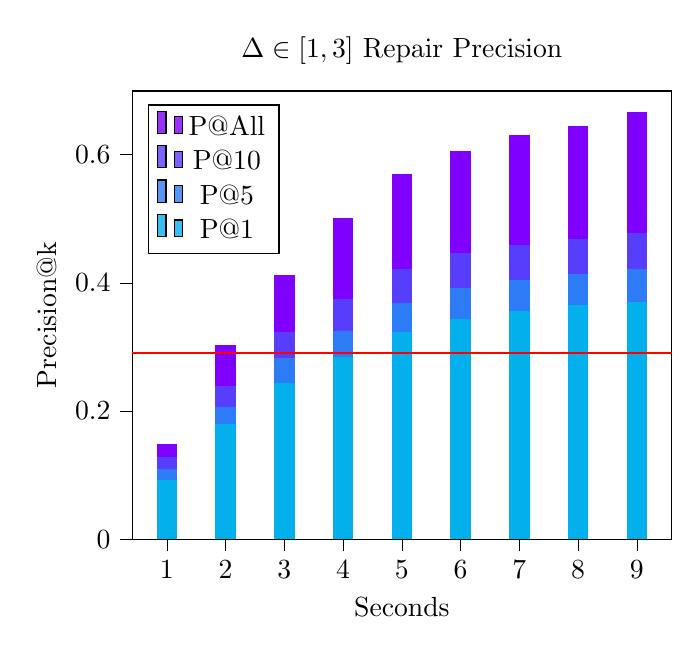
\begin{tikzpicture}

\definecolor{darkgray176}{RGB}{176,176,176}
\definecolor{darkviolet1270255}{RGB}{127,0,255}
\definecolor{deepskyblue3176236}{RGB}{3,176,236}
\definecolor{dodgerblue45123246}{RGB}{45,123,246}
\definecolor{royalblue8762253}{RGB}{87,62,253}

\begin{axis}[
tick align=outside,
tick pos=left,
title={\(\displaystyle \Delta\in[1,3]\) Repair Precision},
legend style={fill opacity=0.8, draw opacity=1, text opacity=1, legend columns=1, legend pos=north west},
x grid style={darkgray176},
xlabel={Seconds},
xmin=-0.5925, xmax=8.5925,
xtick style={color=black},
xtick={0,1,2,3,4,5,6,7,8},
xticklabels={1,2,3,4,5,6,7,8,9},
y grid style={darkgray176},
ylabel={Precision@k},
ymin=0, ymax=0.6993,
ytick style={color=black}
]
\draw[draw=none,fill=darkviolet1270255] (axis cs:-0.175,0) rectangle (axis cs:0.175,0.149);
\addlegendimage{ybar,ybar legend,draw=none,fill=darkviolet1270255}
\addlegendentry{P@All}

\draw[draw=none,fill=darkviolet1270255] (axis cs:0.825,0) rectangle (axis cs:1.175,0.303);
\draw[draw=none,fill=darkviolet1270255] (axis cs:1.825,0) rectangle (axis cs:2.175,0.412);
\draw[draw=none,fill=darkviolet1270255] (axis cs:2.825,0) rectangle (axis cs:3.175,0.501);
\draw[draw=none,fill=darkviolet1270255] (axis cs:3.825,0) rectangle (axis cs:4.175,0.569);
\draw[draw=none,fill=darkviolet1270255] (axis cs:4.825,0) rectangle (axis cs:5.175,0.605);
\draw[draw=none,fill=darkviolet1270255] (axis cs:5.825,0) rectangle (axis cs:6.175,0.63);
\draw[draw=none,fill=darkviolet1270255] (axis cs:6.825,0) rectangle (axis cs:7.175,0.645);
\draw[draw=none,fill=darkviolet1270255] (axis cs:7.825,0) rectangle (axis cs:8.175,0.666);
\draw[draw=none,fill=royalblue8762253] (axis cs:-0.175,0) rectangle (axis cs:0.175,0.128);
\addlegendimage{ybar,ybar legend,draw=none,fill=royalblue8762253}
\addlegendentry{P@10}

\draw[draw=none,fill=royalblue8762253] (axis cs:0.825,0) rectangle (axis cs:1.175,0.239);
\draw[draw=none,fill=royalblue8762253] (axis cs:1.825,0) rectangle (axis cs:2.175,0.323);
\draw[draw=none,fill=royalblue8762253] (axis cs:2.825,0) rectangle (axis cs:3.175,0.374);
\draw[draw=none,fill=royalblue8762253] (axis cs:3.825,0) rectangle (axis cs:4.175,0.421);
\draw[draw=none,fill=royalblue8762253] (axis cs:4.825,0) rectangle (axis cs:5.175,0.446);
\draw[draw=none,fill=royalblue8762253] (axis cs:5.825,0) rectangle (axis cs:6.175,0.459);
\draw[draw=none,fill=royalblue8762253] (axis cs:6.825,0) rectangle (axis cs:7.175,0.469);
\draw[draw=none,fill=royalblue8762253] (axis cs:7.825,0) rectangle (axis cs:8.175,0.477);
\draw[draw=none,fill=dodgerblue45123246] (axis cs:-0.175,0) rectangle (axis cs:0.175,0.11);
\addlegendimage{ybar,ybar legend,draw=none,fill=dodgerblue45123246}
\addlegendentry{P@5}

\draw[draw=none,fill=dodgerblue45123246] (axis cs:0.825,0) rectangle (axis cs:1.175,0.206);
\draw[draw=none,fill=dodgerblue45123246] (axis cs:1.825,0) rectangle (axis cs:2.175,0.282);
\draw[draw=none,fill=dodgerblue45123246] (axis cs:2.825,0) rectangle (axis cs:3.175,0.325);
\draw[draw=none,fill=dodgerblue45123246] (axis cs:3.825,0) rectangle (axis cs:4.175,0.369);
\draw[draw=none,fill=dodgerblue45123246] (axis cs:4.825,0) rectangle (axis cs:5.175,0.392);
\draw[draw=none,fill=dodgerblue45123246] (axis cs:5.825,0) rectangle (axis cs:6.175,0.405);
\draw[draw=none,fill=dodgerblue45123246] (axis cs:6.825,0) rectangle (axis cs:7.175,0.414);
\draw[draw=none,fill=dodgerblue45123246] (axis cs:7.825,0) rectangle (axis cs:8.175,0.422);
\draw[draw=none,fill=deepskyblue3176236] (axis cs:-0.175,0) rectangle (axis cs:0.175,0.092);
\addlegendimage{ybar,ybar legend,draw=none,fill=deepskyblue3176236}
\addlegendentry{P@1}

\draw[draw=none,fill=deepskyblue3176236] (axis cs:0.825,0) rectangle (axis cs:1.175,0.18);
\draw[draw=none,fill=deepskyblue3176236] (axis cs:1.825,0) rectangle (axis cs:2.175,0.244);
\draw[draw=none,fill=deepskyblue3176236] (axis cs:2.825,0) rectangle (axis cs:3.175,0.285);
\draw[draw=none,fill=deepskyblue3176236] (axis cs:3.825,0) rectangle (axis cs:4.175,0.324);
\draw[draw=none,fill=deepskyblue3176236] (axis cs:4.825,0) rectangle (axis cs:5.175,0.343);
\draw[draw=none,fill=deepskyblue3176236] (axis cs:5.825,0) rectangle (axis cs:6.175,0.356);
\draw[draw=none,fill=deepskyblue3176236] (axis cs:6.825,0) rectangle (axis cs:7.175,0.365);
\draw[draw=none,fill=deepskyblue3176236] (axis cs:7.825,0) rectangle (axis cs:8.175,0.37);
\addplot [red, thick] coordinates {(-0.8925,0.29) (14.8925,0.29)};
\end{axis}

\end{tikzpicture}
}
  \resizebox{.24\textwidth}{!}{% This file was created with tikzplotlib v0.10.1.
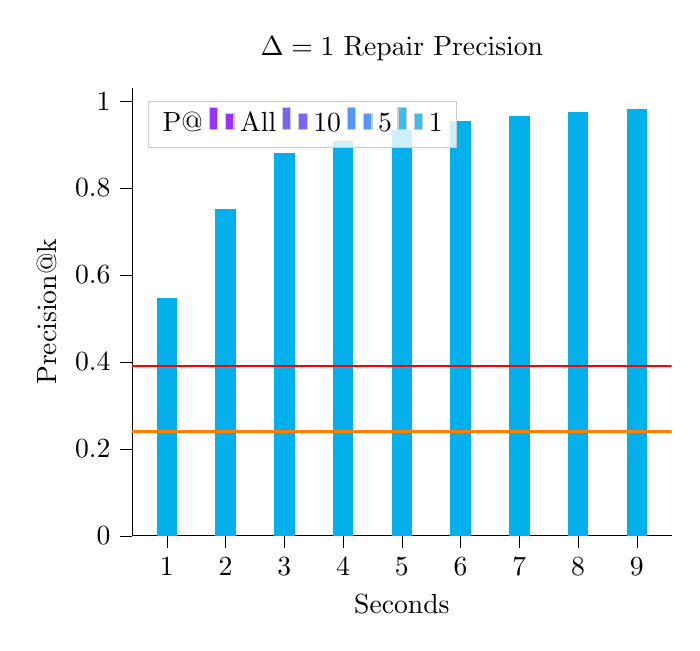
\begin{tikzpicture}
\begin{axis}[
legend cell align={left},
legend style={fill opacity=0.8, draw opacity=1, text opacity=1, draw=lightgray204, legend columns=-1, legend pos=north west},
tick align=outside,
tick pos=left,
axis lines*=left,
title={\(\displaystyle \Delta=1\) Repair Precision},
x grid style={darkgray176},
xlabel={Seconds},
xmin=-0.5925, xmax=8.5925,
xtick style={color=black},
xtick={0,1,2,3,4,5,6,7,8},
xticklabels={1,2,3,4,5,6,7,8,9},
y grid style={darkgray176},
ylabel={Precision@k},
ymin=0, ymax=1.0311,
ytick style={color=black}
]
\draw[draw=none,fill=darkviolet1270255] (axis cs:-0.175,0) rectangle (axis cs:0.175,0.546);
\addlegendimage{empty legend}
\addlegendentry{P@}
\addlegendimage{ybar,ybar legend,draw=none,fill=darkviolet1270255}
\addlegendentry{All}
\addlegendimage{ybar,ybar legend,draw=none,fill=royalblue8762253}
\addlegendentry{10}
\addlegendimage{ybar,ybar legend,draw=none,fill=dodgerblue45123246}
\addlegendentry{5}
\addlegendimage{ybar,ybar legend,draw=none,fill=deepskyblue3176236}
\addlegendentry{1}

\draw[draw=none,fill=darkviolet1270255] (axis cs:0.825,0) rectangle (axis cs:1.175,0.752);
\draw[draw=none,fill=darkviolet1270255] (axis cs:1.825,0) rectangle (axis cs:2.175,0.88);
\draw[draw=none,fill=darkviolet1270255] (axis cs:2.825,0) rectangle (axis cs:3.175,0.908);
\draw[draw=none,fill=darkviolet1270255] (axis cs:3.825,0) rectangle (axis cs:4.175,0.933);
\draw[draw=none,fill=darkviolet1270255] (axis cs:4.825,0) rectangle (axis cs:5.175,0.954);
\draw[draw=none,fill=darkviolet1270255] (axis cs:5.825,0) rectangle (axis cs:6.175,0.966);
\draw[draw=none,fill=darkviolet1270255] (axis cs:6.825,0) rectangle (axis cs:7.175,0.975);
\draw[draw=none,fill=darkviolet1270255] (axis cs:7.825,0) rectangle (axis cs:8.175,0.982);
\draw[draw=none,fill=royalblue8762253] (axis cs:-0.175,0) rectangle (axis cs:0.175,0.546);

\draw[draw=none,fill=royalblue8762253] (axis cs:0.825,0) rectangle (axis cs:1.175,0.752);
\draw[draw=none,fill=royalblue8762253] (axis cs:1.825,0) rectangle (axis cs:2.175,0.88);
\draw[draw=none,fill=royalblue8762253] (axis cs:2.825,0) rectangle (axis cs:3.175,0.908);
\draw[draw=none,fill=royalblue8762253] (axis cs:3.825,0) rectangle (axis cs:4.175,0.933);
\draw[draw=none,fill=royalblue8762253] (axis cs:4.825,0) rectangle (axis cs:5.175,0.954);
\draw[draw=none,fill=royalblue8762253] (axis cs:5.825,0) rectangle (axis cs:6.175,0.966);
\draw[draw=none,fill=royalblue8762253] (axis cs:6.825,0) rectangle (axis cs:7.175,0.975);
\draw[draw=none,fill=royalblue8762253] (axis cs:7.825,0) rectangle (axis cs:8.175,0.982);
\draw[draw=none,fill=dodgerblue45123246] (axis cs:-0.175,0) rectangle (axis cs:0.175,0.546);

\draw[draw=none,fill=dodgerblue45123246] (axis cs:0.825,0) rectangle (axis cs:1.175,0.752);
\draw[draw=none,fill=dodgerblue45123246] (axis cs:1.825,0) rectangle (axis cs:2.175,0.88);
\draw[draw=none,fill=dodgerblue45123246] (axis cs:2.825,0) rectangle (axis cs:3.175,0.908);
\draw[draw=none,fill=dodgerblue45123246] (axis cs:3.825,0) rectangle (axis cs:4.175,0.933);
\draw[draw=none,fill=dodgerblue45123246] (axis cs:4.825,0) rectangle (axis cs:5.175,0.954);
\draw[draw=none,fill=dodgerblue45123246] (axis cs:5.825,0) rectangle (axis cs:6.175,0.966);
\draw[draw=none,fill=dodgerblue45123246] (axis cs:6.825,0) rectangle (axis cs:7.175,0.975);
\draw[draw=none,fill=dodgerblue45123246] (axis cs:7.825,0) rectangle (axis cs:8.175,0.982);
\draw[draw=none,fill=deepskyblue3176236] (axis cs:-0.175,0) rectangle (axis cs:0.175,0.546);

\draw[draw=none,fill=deepskyblue3176236] (axis cs:0.825,0) rectangle (axis cs:1.175,0.752);
\draw[draw=none,fill=deepskyblue3176236] (axis cs:1.825,0) rectangle (axis cs:2.175,0.88);
\draw[draw=none,fill=deepskyblue3176236] (axis cs:2.825,0) rectangle (axis cs:3.175,0.908);
\draw[draw=none,fill=deepskyblue3176236] (axis cs:3.825,0) rectangle (axis cs:4.175,0.933);
\draw[draw=none,fill=deepskyblue3176236] (axis cs:4.825,0) rectangle (axis cs:5.175,0.954);
\draw[draw=none,fill=deepskyblue3176236] (axis cs:5.825,0) rectangle (axis cs:6.175,0.966);
\draw[draw=none,fill=deepskyblue3176236] (axis cs:6.825,0) rectangle (axis cs:7.175,0.975);
\draw[draw=none,fill=deepskyblue3176236] (axis cs:7.825,0) rectangle (axis cs:8.175,0.982);
\addplot [red, thick] coordinates {(-0.8925,0.39) (14.8925,0.39)};
\addplot [orange, thick] coordinates {(-0.8925,0.24) (14.8925,0.24)};
\end{axis}

\end{tikzpicture}
}
  \resizebox{.24\textwidth}{!}{% This file was created with tikzplotlib v0.10.1.
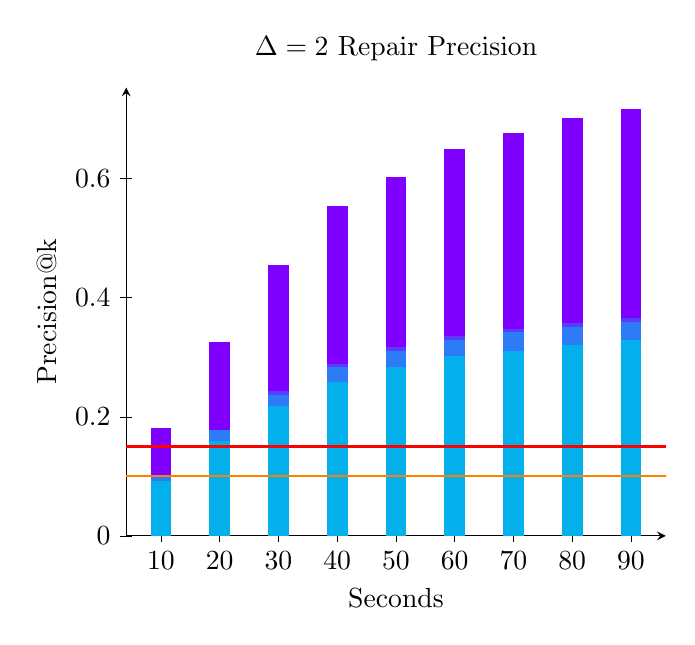
\begin{tikzpicture}
\begin{axis}[
tick align=outside,
tick pos=left,
axis lines=left,
title={\(\displaystyle \Delta=2\) Repair Precision},
x grid style={darkgray176},
xlabel={Seconds},
xmin=-0.5925, xmax=8.5925,
xtick style={color=black},
xtick={0,1,2,3,4,5,6,7,8},
xticklabels={10,20,30,40,50,60,70,80,90},
y grid style={darkgray176},
ylabel={Precision@k},
ymin=0, ymax=0.75285,
ytick style={color=black}
]

\draw[draw=none,fill=darkviolet1270255] (axis cs:-0.175,0) rectangle (axis cs:0.175,0.182);

\draw[draw=none,fill=darkviolet1270255] (axis cs:0.825,0) rectangle (axis cs:1.175,0.326);
\draw[draw=none,fill=darkviolet1270255] (axis cs:1.825,0) rectangle (axis cs:2.175,0.455);
\draw[draw=none,fill=darkviolet1270255] (axis cs:2.825,0) rectangle (axis cs:3.175,0.554);
\draw[draw=none,fill=darkviolet1270255] (axis cs:3.825,0) rectangle (axis cs:4.175,0.603);
\draw[draw=none,fill=darkviolet1270255] (axis cs:4.825,0) rectangle (axis cs:5.175,0.649);
\draw[draw=none,fill=darkviolet1270255] (axis cs:5.825,0) rectangle (axis cs:6.175,0.677);
\draw[draw=none,fill=darkviolet1270255] (axis cs:6.825,0) rectangle (axis cs:7.175,0.702);
\draw[draw=none,fill=darkviolet1270255] (axis cs:7.825,0) rectangle (axis cs:8.175,0.717);
\draw[draw=none,fill=royalblue8762253] (axis cs:-0.175,0) rectangle (axis cs:0.175,0.102);

\draw[draw=none,fill=royalblue8762253] (axis cs:0.825,0) rectangle (axis cs:1.175,0.178);
\draw[draw=none,fill=royalblue8762253] (axis cs:1.825,0) rectangle (axis cs:2.175,0.243);
\draw[draw=none,fill=royalblue8762253] (axis cs:2.825,0) rectangle (axis cs:3.175,0.289);
\draw[draw=none,fill=royalblue8762253] (axis cs:3.825,0) rectangle (axis cs:4.175,0.317);
\draw[draw=none,fill=royalblue8762253] (axis cs:4.825,0) rectangle (axis cs:5.175,0.335);
\draw[draw=none,fill=royalblue8762253] (axis cs:5.825,0) rectangle (axis cs:6.175,0.348);
\draw[draw=none,fill=royalblue8762253] (axis cs:6.825,0) rectangle (axis cs:7.175,0.357);
\draw[draw=none,fill=royalblue8762253] (axis cs:7.825,0) rectangle (axis cs:8.175,0.366);
\draw[draw=none,fill=dodgerblue45123246] (axis cs:-0.175,0) rectangle (axis cs:0.175,0.102);

\draw[draw=none,fill=dodgerblue45123246] (axis cs:0.825,0) rectangle (axis cs:1.175,0.178);
\draw[draw=none,fill=dodgerblue45123246] (axis cs:1.825,0) rectangle (axis cs:2.175,0.237);
\draw[draw=none,fill=dodgerblue45123246] (axis cs:2.825,0) rectangle (axis cs:3.175,0.283);
\draw[draw=none,fill=dodgerblue45123246] (axis cs:3.825,0) rectangle (axis cs:4.175,0.311);
\draw[draw=none,fill=dodgerblue45123246] (axis cs:4.825,0) rectangle (axis cs:5.175,0.329);
\draw[draw=none,fill=dodgerblue45123246] (axis cs:5.825,0) rectangle (axis cs:6.175,0.342);
\draw[draw=none,fill=dodgerblue45123246] (axis cs:6.825,0) rectangle (axis cs:7.175,0.351);
\draw[draw=none,fill=dodgerblue45123246] (axis cs:7.825,0) rectangle (axis cs:8.175,0.36);
\draw[draw=none,fill=deepskyblue3176236] (axis cs:-0.175,0) rectangle (axis cs:0.175,0.092);

\draw[draw=none,fill=deepskyblue3176236] (axis cs:0.825,0) rectangle (axis cs:1.175,0.16);
\draw[draw=none,fill=deepskyblue3176236] (axis cs:1.825,0) rectangle (axis cs:2.175,0.218);
\draw[draw=none,fill=deepskyblue3176236] (axis cs:2.825,0) rectangle (axis cs:3.175,0.258);
\draw[draw=none,fill=deepskyblue3176236] (axis cs:3.825,0) rectangle (axis cs:4.175,0.283);
\draw[draw=none,fill=deepskyblue3176236] (axis cs:4.825,0) rectangle (axis cs:5.175,0.302);
\draw[draw=none,fill=deepskyblue3176236] (axis cs:5.825,0) rectangle (axis cs:6.175,0.311);
\draw[draw=none,fill=deepskyblue3176236] (axis cs:6.825,0) rectangle (axis cs:7.175,0.32);
\draw[draw=none,fill=deepskyblue3176236] (axis cs:7.825,0) rectangle (axis cs:8.175,0.329);
\addplot [red, thick] coordinates {(-0.8925,0.15) (14.8925,0.15)};
\addplot [orange, thick] coordinates {(-0.8925,0.10) (14.8925,0.10)};
\end{axis}

\end{tikzpicture}
}
  \resizebox{.24\textwidth}{!}{% This file was created with tikzplotlib v0.10.1.
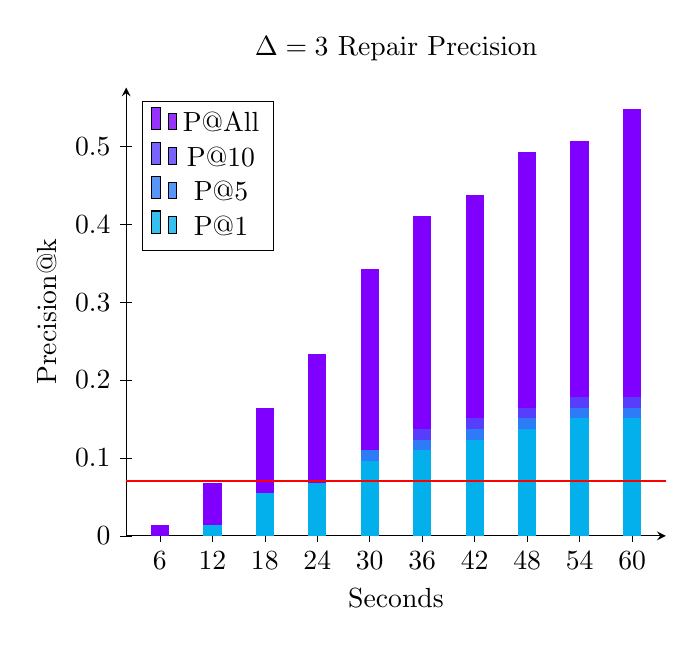
\begin{tikzpicture}

\definecolor{darkgray176}{RGB}{176,176,176}
\definecolor{darkviolet1270255}{RGB}{127,0,255}
\definecolor{deepskyblue3176236}{RGB}{3,176,236}
\definecolor{dodgerblue45123246}{RGB}{45,123,246}
\definecolor{royalblue8762253}{RGB}{87,62,253}

\begin{axis}[
tick align=outside,
tick pos=left,
axis lines=left,
title={\(\displaystyle \Delta=3\) Repair Precision},
legend style={fill opacity=0.8, draw opacity=1, text opacity=1, legend columns=1, legend pos=north west},
x grid style={darkgray176},
xlabel={Seconds},
xmin=-0.6425, xmax=9.6425,
xtick style={color=black},
xtick={0,1,2,3,4,5,6,7,8,9},
xticklabels={6,12,18,24,30,36,42,48,54,60},
y grid style={darkgray176},
ylabel={Precision@k},
ymin=0, ymax=0.5754,
ytick style={color=black}
]
\draw[draw=none,fill=darkviolet1270255] (axis cs:-0.175,0) rectangle (axis cs:0.175,0.014);
\addlegendimage{ybar,ybar legend,draw=none,fill=darkviolet1270255}
\addlegendentry{P@All}

\draw[draw=none,fill=darkviolet1270255] (axis cs:0.825,0) rectangle (axis cs:1.175,0.068);
\draw[draw=none,fill=darkviolet1270255] (axis cs:1.825,0) rectangle (axis cs:2.175,0.164);
\draw[draw=none,fill=darkviolet1270255] (axis cs:2.825,0) rectangle (axis cs:3.175,0.233);
\draw[draw=none,fill=darkviolet1270255] (axis cs:3.825,0) rectangle (axis cs:4.175,0.342);
\draw[draw=none,fill=darkviolet1270255] (axis cs:4.825,0) rectangle (axis cs:5.175,0.411);
\draw[draw=none,fill=darkviolet1270255] (axis cs:5.825,0) rectangle (axis cs:6.175,0.438);
\draw[draw=none,fill=darkviolet1270255] (axis cs:6.825,0) rectangle (axis cs:7.175,0.493);
\draw[draw=none,fill=darkviolet1270255] (axis cs:7.825,0) rectangle (axis cs:8.175,0.507);
\draw[draw=none,fill=darkviolet1270255] (axis cs:8.825,0) rectangle (axis cs:9.175,0.548);
\draw[draw=none,fill=royalblue8762253] (axis cs:-0.175,0) rectangle (axis cs:0.175,0);
\addlegendimage{ybar,ybar legend,draw=none,fill=royalblue8762253}
\addlegendentry{P@10}

\draw[draw=none,fill=royalblue8762253] (axis cs:0.825,0) rectangle (axis cs:1.175,0.014);
\draw[draw=none,fill=royalblue8762253] (axis cs:1.825,0) rectangle (axis cs:2.175,0.055);
\draw[draw=none,fill=royalblue8762253] (axis cs:2.825,0) rectangle (axis cs:3.175,0.068);
\draw[draw=none,fill=royalblue8762253] (axis cs:3.825,0) rectangle (axis cs:4.175,0.11);
\draw[draw=none,fill=royalblue8762253] (axis cs:4.825,0) rectangle (axis cs:5.175,0.137);
\draw[draw=none,fill=royalblue8762253] (axis cs:5.825,0) rectangle (axis cs:6.175,0.151);
\draw[draw=none,fill=royalblue8762253] (axis cs:6.825,0) rectangle (axis cs:7.175,0.164);
\draw[draw=none,fill=royalblue8762253] (axis cs:7.825,0) rectangle (axis cs:8.175,0.178);
\draw[draw=none,fill=royalblue8762253] (axis cs:8.825,0) rectangle (axis cs:9.175,0.178);
\draw[draw=none,fill=dodgerblue45123246] (axis cs:-0.175,0) rectangle (axis cs:0.175,0);
\addlegendimage{ybar,ybar legend,draw=none,fill=dodgerblue45123246}
\addlegendentry{P@5}

\draw[draw=none,fill=dodgerblue45123246] (axis cs:0.825,0) rectangle (axis cs:1.175,0.014);
\draw[draw=none,fill=dodgerblue45123246] (axis cs:1.825,0) rectangle (axis cs:2.175,0.055);
\draw[draw=none,fill=dodgerblue45123246] (axis cs:2.825,0) rectangle (axis cs:3.175,0.068);
\draw[draw=none,fill=dodgerblue45123246] (axis cs:3.825,0) rectangle (axis cs:4.175,0.11);
\draw[draw=none,fill=dodgerblue45123246] (axis cs:4.825,0) rectangle (axis cs:5.175,0.123);
\draw[draw=none,fill=dodgerblue45123246] (axis cs:5.825,0) rectangle (axis cs:6.175,0.137);
\draw[draw=none,fill=dodgerblue45123246] (axis cs:6.825,0) rectangle (axis cs:7.175,0.151);
\draw[draw=none,fill=dodgerblue45123246] (axis cs:7.825,0) rectangle (axis cs:8.175,0.164);
\draw[draw=none,fill=dodgerblue45123246] (axis cs:8.825,0) rectangle (axis cs:9.175,0.164);
\draw[draw=none,fill=deepskyblue3176236] (axis cs:-0.175,0) rectangle (axis cs:0.175,0);
\addlegendimage{ybar,ybar legend,draw=none,fill=deepskyblue3176236}
\addlegendentry{P@1}

\draw[draw=none,fill=deepskyblue3176236] (axis cs:0.825,0) rectangle (axis cs:1.175,0.014);
\draw[draw=none,fill=deepskyblue3176236] (axis cs:1.825,0) rectangle (axis cs:2.175,0.055);
\draw[draw=none,fill=deepskyblue3176236] (axis cs:2.825,0) rectangle (axis cs:3.175,0.068);
\draw[draw=none,fill=deepskyblue3176236] (axis cs:3.825,0) rectangle (axis cs:4.175,0.096);
\draw[draw=none,fill=deepskyblue3176236] (axis cs:4.825,0) rectangle (axis cs:5.175,0.11);
\draw[draw=none,fill=deepskyblue3176236] (axis cs:5.825,0) rectangle (axis cs:6.175,0.123);
\draw[draw=none,fill=deepskyblue3176236] (axis cs:6.825,0) rectangle (axis cs:7.175,0.137);
\draw[draw=none,fill=deepskyblue3176236] (axis cs:7.825,0) rectangle (axis cs:8.175,0.151);
\draw[draw=none,fill=deepskyblue3176236] (axis cs:8.825,0) rectangle (axis cs:9.175,0.151);
\addplot [red, thick] coordinates {(-0.8925,0.07) (14.8925,0.07)};
\end{axis}

\end{tikzpicture}
}
  \resizebox{.24\textwidth}{!}{% This file was created with tikzplotlib v0.10.1.
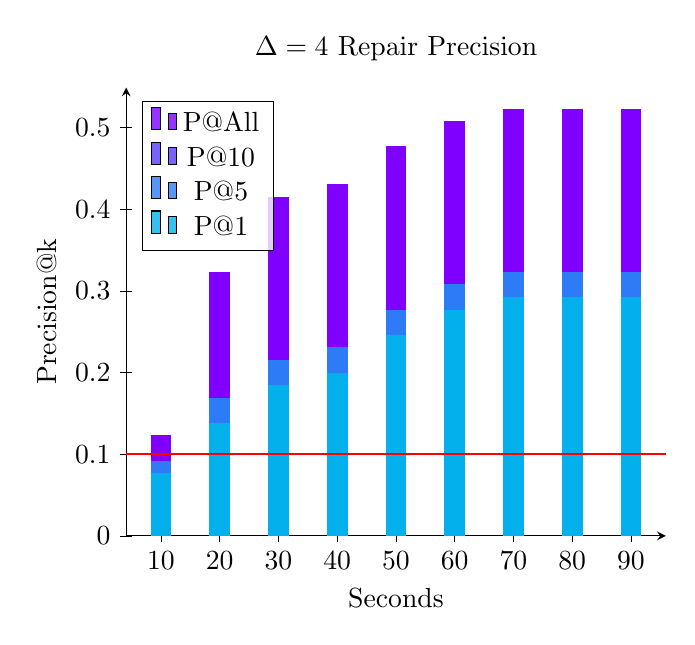
\begin{tikzpicture}

\definecolor{darkgray176}{RGB}{176,176,176}
\definecolor{darkviolet1270255}{RGB}{127,0,255}
\definecolor{deepskyblue3176236}{RGB}{3,176,236}
\definecolor{dodgerblue45123246}{RGB}{45,123,246}
\definecolor{royalblue8762253}{RGB}{87,62,253}

\begin{axis}[
tick align=outside,
tick pos=left,
axis lines=left,
title={\(\displaystyle \Delta=4\) Repair Precision},
legend style={fill opacity=0.8, draw opacity=1, text opacity=1, legend columns=1, legend pos=north west},
x grid style={darkgray176},
xlabel={Seconds},
xmin=-0.5925, xmax=8.5925,
xtick style={color=black},
xtick={0,1,2,3,4,5,6,7,8},
xticklabels={10,20,30,40,50,60,70,80,90},
y grid style={darkgray176},
ylabel={Precision@k},
ymin=0, ymax=0.54915,
ytick style={color=black}
]
\draw[draw=none,fill=darkviolet1270255] (axis cs:-0.175,0) rectangle (axis cs:0.175,0.123);
\addlegendimage{ybar,ybar legend,draw=none,fill=darkviolet1270255}
\addlegendentry{P@All}

\draw[draw=none,fill=darkviolet1270255] (axis cs:0.825,0) rectangle (axis cs:1.175,0.323);
\draw[draw=none,fill=darkviolet1270255] (axis cs:1.825,0) rectangle (axis cs:2.175,0.415);
\draw[draw=none,fill=darkviolet1270255] (axis cs:2.825,0) rectangle (axis cs:3.175,0.431);
\draw[draw=none,fill=darkviolet1270255] (axis cs:3.825,0) rectangle (axis cs:4.175,0.477);
\draw[draw=none,fill=darkviolet1270255] (axis cs:4.825,0) rectangle (axis cs:5.175,0.508);
\draw[draw=none,fill=darkviolet1270255] (axis cs:5.825,0) rectangle (axis cs:6.175,0.523);
\draw[draw=none,fill=darkviolet1270255] (axis cs:6.825,0) rectangle (axis cs:7.175,0.523);
\draw[draw=none,fill=darkviolet1270255] (axis cs:7.825,0) rectangle (axis cs:8.175,0.523);
\draw[draw=none,fill=royalblue8762253] (axis cs:-0.175,0) rectangle (axis cs:0.175,0.092);
\addlegendimage{ybar,ybar legend,draw=none,fill=royalblue8762253}
\addlegendentry{P@10}

\draw[draw=none,fill=royalblue8762253] (axis cs:0.825,0) rectangle (axis cs:1.175,0.169);
\draw[draw=none,fill=royalblue8762253] (axis cs:1.825,0) rectangle (axis cs:2.175,0.215);
\draw[draw=none,fill=royalblue8762253] (axis cs:2.825,0) rectangle (axis cs:3.175,0.231);
\draw[draw=none,fill=royalblue8762253] (axis cs:3.825,0) rectangle (axis cs:4.175,0.277);
\draw[draw=none,fill=royalblue8762253] (axis cs:4.825,0) rectangle (axis cs:5.175,0.308);
\draw[draw=none,fill=royalblue8762253] (axis cs:5.825,0) rectangle (axis cs:6.175,0.323);
\draw[draw=none,fill=royalblue8762253] (axis cs:6.825,0) rectangle (axis cs:7.175,0.323);
\draw[draw=none,fill=royalblue8762253] (axis cs:7.825,0) rectangle (axis cs:8.175,0.323);
\draw[draw=none,fill=dodgerblue45123246] (axis cs:-0.175,0) rectangle (axis cs:0.175,0.092);
\addlegendimage{ybar,ybar legend,draw=none,fill=dodgerblue45123246}
\addlegendentry{P@5}

\draw[draw=none,fill=dodgerblue45123246] (axis cs:0.825,0) rectangle (axis cs:1.175,0.169);
\draw[draw=none,fill=dodgerblue45123246] (axis cs:1.825,0) rectangle (axis cs:2.175,0.215);
\draw[draw=none,fill=dodgerblue45123246] (axis cs:2.825,0) rectangle (axis cs:3.175,0.231);
\draw[draw=none,fill=dodgerblue45123246] (axis cs:3.825,0) rectangle (axis cs:4.175,0.277);
\draw[draw=none,fill=dodgerblue45123246] (axis cs:4.825,0) rectangle (axis cs:5.175,0.308);
\draw[draw=none,fill=dodgerblue45123246] (axis cs:5.825,0) rectangle (axis cs:6.175,0.323);
\draw[draw=none,fill=dodgerblue45123246] (axis cs:6.825,0) rectangle (axis cs:7.175,0.323);
\draw[draw=none,fill=dodgerblue45123246] (axis cs:7.825,0) rectangle (axis cs:8.175,0.323);
\draw[draw=none,fill=deepskyblue3176236] (axis cs:-0.175,0) rectangle (axis cs:0.175,0.077);
\addlegendimage{ybar,ybar legend,draw=none,fill=deepskyblue3176236}
\addlegendentry{P@1}

\draw[draw=none,fill=deepskyblue3176236] (axis cs:0.825,0) rectangle (axis cs:1.175,0.138);
\draw[draw=none,fill=deepskyblue3176236] (axis cs:1.825,0) rectangle (axis cs:2.175,0.185);
\draw[draw=none,fill=deepskyblue3176236] (axis cs:2.825,0) rectangle (axis cs:3.175,0.2);
\draw[draw=none,fill=deepskyblue3176236] (axis cs:3.825,0) rectangle (axis cs:4.175,0.246);
\draw[draw=none,fill=deepskyblue3176236] (axis cs:4.825,0) rectangle (axis cs:5.175,0.277);
\draw[draw=none,fill=deepskyblue3176236] (axis cs:5.825,0) rectangle (axis cs:6.175,0.292);
\draw[draw=none,fill=deepskyblue3176236] (axis cs:6.825,0) rectangle (axis cs:7.175,0.292);
\draw[draw=none,fill=deepskyblue3176236] (axis cs:7.825,0) rectangle (axis cs:8.175,0.292);
\addplot [red, thick] coordinates {(-0.8925,0.10) (14.8925,0.10)};
\end{axis}

\end{tikzpicture}
}
%    \resizebox{.24\textwidth}{!}{% This file was created with tikzplotlib v0.10.1.
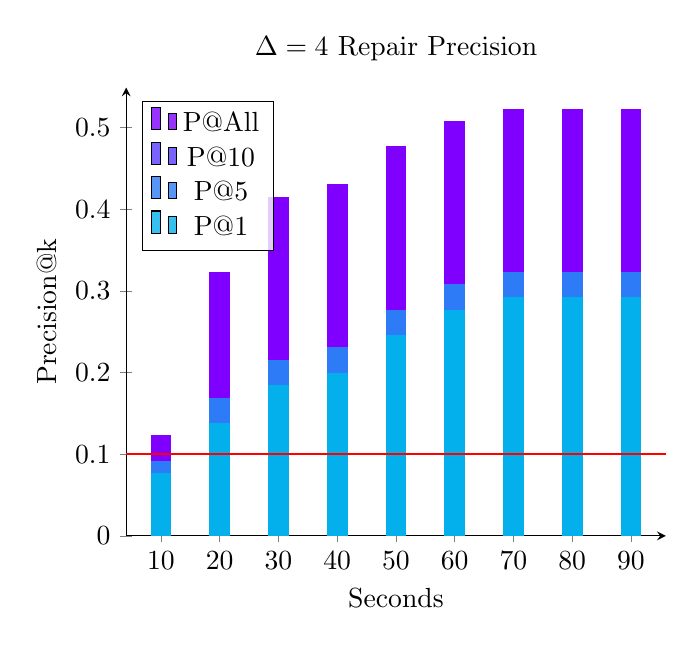
\begin{tikzpicture}

\definecolor{darkgray176}{RGB}{176,176,176}
\definecolor{darkviolet1270255}{RGB}{127,0,255}
\definecolor{deepskyblue3176236}{RGB}{3,176,236}
\definecolor{dodgerblue45123246}{RGB}{45,123,246}
\definecolor{royalblue8762253}{RGB}{87,62,253}

\begin{axis}[
tick align=outside,
tick pos=left,
axis lines=left,
title={\(\displaystyle \Delta=4\) Repair Precision},
legend style={fill opacity=0.8, draw opacity=1, text opacity=1, legend columns=1, legend pos=north west},
x grid style={darkgray176},
xlabel={Seconds},
xmin=-0.5925, xmax=8.5925,
xtick={0,1,2,3,4,5,6,7,8},
xticklabels={10,20,30,40,50,60,70,80,90},
y grid style={darkgray176},
ylabel={Precision@k},
ymin=0, ymax=0.54915,
]
\draw[draw=none,fill=darkviolet1270255] (axis cs:-0.175,0) rectangle (axis cs:0.175,0.123);
\addlegendimage{ybar,ybar legend,draw=none,fill=darkviolet1270255}
\addlegendentry{P@All}

\draw[draw=none,fill=darkviolet1270255] (axis cs:0.825,0) rectangle (axis cs:1.175,0.323);
\draw[draw=none,fill=darkviolet1270255] (axis cs:1.825,0) rectangle (axis cs:2.175,0.415);
\draw[draw=none,fill=darkviolet1270255] (axis cs:2.825,0) rectangle (axis cs:3.175,0.431);
\draw[draw=none,fill=darkviolet1270255] (axis cs:3.825,0) rectangle (axis cs:4.175,0.477);
\draw[draw=none,fill=darkviolet1270255] (axis cs:4.825,0) rectangle (axis cs:5.175,0.508);
\draw[draw=none,fill=darkviolet1270255] (axis cs:5.825,0) rectangle (axis cs:6.175,0.523);
\draw[draw=none,fill=darkviolet1270255] (axis cs:6.825,0) rectangle (axis cs:7.175,0.523);
\draw[draw=none,fill=darkviolet1270255] (axis cs:7.825,0) rectangle (axis cs:8.175,0.523);
\draw[draw=none,fill=royalblue8762253] (axis cs:-0.175,0) rectangle (axis cs:0.175,0.092);
\addlegendimage{ybar,ybar legend,draw=none,fill=royalblue8762253}
\addlegendentry{P@10}

\draw[draw=none,fill=royalblue8762253] (axis cs:0.825,0) rectangle (axis cs:1.175,0.169);
\draw[draw=none,fill=royalblue8762253] (axis cs:1.825,0) rectangle (axis cs:2.175,0.215);
\draw[draw=none,fill=royalblue8762253] (axis cs:2.825,0) rectangle (axis cs:3.175,0.231);
\draw[draw=none,fill=royalblue8762253] (axis cs:3.825,0) rectangle (axis cs:4.175,0.277);
\draw[draw=none,fill=royalblue8762253] (axis cs:4.825,0) rectangle (axis cs:5.175,0.308);
\draw[draw=none,fill=royalblue8762253] (axis cs:5.825,0) rectangle (axis cs:6.175,0.323);
\draw[draw=none,fill=royalblue8762253] (axis cs:6.825,0) rectangle (axis cs:7.175,0.323);
\draw[draw=none,fill=royalblue8762253] (axis cs:7.825,0) rectangle (axis cs:8.175,0.323);
\draw[draw=none,fill=dodgerblue45123246] (axis cs:-0.175,0) rectangle (axis cs:0.175,0.092);
\addlegendimage{ybar,ybar legend,draw=none,fill=dodgerblue45123246}
\addlegendentry{P@5}

\draw[draw=none,fill=dodgerblue45123246] (axis cs:0.825,0) rectangle (axis cs:1.175,0.169);
\draw[draw=none,fill=dodgerblue45123246] (axis cs:1.825,0) rectangle (axis cs:2.175,0.215);
\draw[draw=none,fill=dodgerblue45123246] (axis cs:2.825,0) rectangle (axis cs:3.175,0.231);
\draw[draw=none,fill=dodgerblue45123246] (axis cs:3.825,0) rectangle (axis cs:4.175,0.277);
\draw[draw=none,fill=dodgerblue45123246] (axis cs:4.825,0) rectangle (axis cs:5.175,0.308);
\draw[draw=none,fill=dodgerblue45123246] (axis cs:5.825,0) rectangle (axis cs:6.175,0.323);
\draw[draw=none,fill=dodgerblue45123246] (axis cs:6.825,0) rectangle (axis cs:7.175,0.323);
\draw[draw=none,fill=dodgerblue45123246] (axis cs:7.825,0) rectangle (axis cs:8.175,0.323);
\draw[draw=none,fill=deepskyblue3176236] (axis cs:-0.175,0) rectangle (axis cs:0.175,0.077);
\addlegendimage{ybar,ybar legend,draw=none,fill=deepskyblue3176236}
\addlegendentry{P@1}

\draw[draw=none,fill=deepskyblue3176236] (axis cs:0.825,0) rectangle (axis cs:1.175,0.138);
\draw[draw=none,fill=deepskyblue3176236] (axis cs:1.825,0) rectangle (axis cs:2.175,0.185);
\draw[draw=none,fill=deepskyblue3176236] (axis cs:2.825,0) rectangle (axis cs:3.175,0.2);
\draw[draw=none,fill=deepskyblue3176236] (axis cs:3.825,0) rectangle (axis cs:4.175,0.246);
\draw[draw=none,fill=deepskyblue3176236] (axis cs:4.825,0) rectangle (axis cs:5.175,0.277);
\draw[draw=none,fill=deepskyblue3176236] (axis cs:5.825,0) rectangle (axis cs:6.175,0.292);
\draw[draw=none,fill=deepskyblue3176236] (axis cs:6.825,0) rectangle (axis cs:7.175,0.292);
\draw[draw=none,fill=deepskyblue3176236] (axis cs:7.825,0) rectangle (axis cs:8.175,0.292);
\addplot [red, thick] coordinates {(-0.8925,0.10) (14.8925,0.10)};
\end{axis}

\end{tikzpicture}
}
%\resizebox{.3\textwidth}{!}{% This file was created with tikzplotlib v0.10.1.
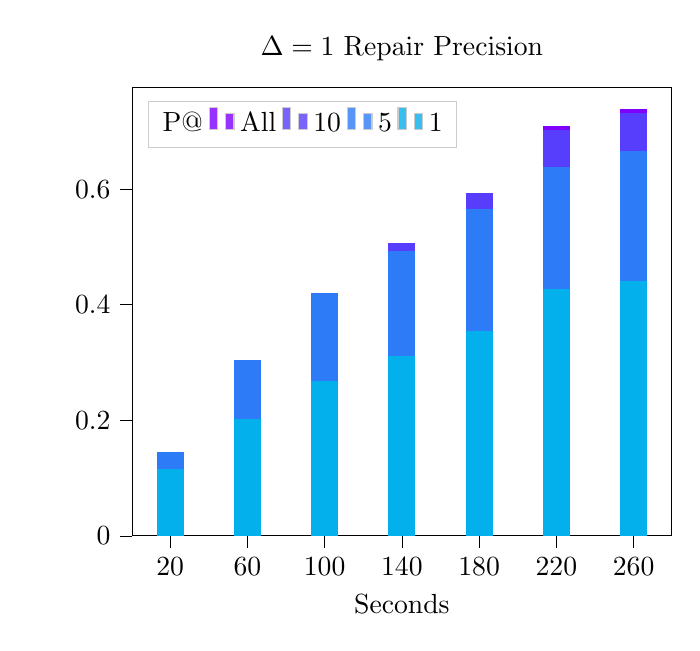
\begin{tikzpicture}

\definecolor{darkgray176}{RGB}{176,176,176}
\definecolor{darkviolet1270255}{RGB}{127,0,255}
\definecolor{deepskyblue3176236}{RGB}{3,176,236}
\definecolor{dodgerblue45123246}{RGB}{45,123,246}
\definecolor{lightgray204}{RGB}{204,204,204}
\definecolor{royalblue8762253}{RGB}{87,62,253}

\begin{axis}[
legend cell align={left},
legend style={fill opacity=0.8, draw opacity=1, text opacity=1, draw=lightgray204, legend columns=-1, legend pos=north west},
tick align=outside,
tick pos=left,
title={$\Delta=1$ Repair Precision},
x grid style={darkgray176},
xlabel={Seconds},
xmin=-0.4925, xmax=6.4925,
xtick style={color=black},
xtick={0,1,2,3,4,5,6},
xticklabels={20,60,100,140,180,220,260},
y grid style={darkgray176},
ylabel={\phantom{Precision@k}},
ymin=0, ymax=0.77595,
ytick style={color=black}
]
\addlegendimage{empty legend}
\addlegendentry{P@}
\draw[draw=none,fill=darkviolet1270255] (axis cs:-0.175,0) rectangle (axis cs:0.175,0.145);
\addlegendimage{ybar,ybar legend,draw=none,fill=darkviolet1270255}
\addlegendentry{All}

\draw[draw=none,fill=darkviolet1270255] (axis cs:0.825,0) rectangle (axis cs:1.175,0.304);
\draw[draw=none,fill=darkviolet1270255] (axis cs:1.825,0) rectangle (axis cs:2.175,0.42);
\draw[draw=none,fill=darkviolet1270255] (axis cs:2.825,0) rectangle (axis cs:3.175,0.507);
\draw[draw=none,fill=darkviolet1270255] (axis cs:3.825,0) rectangle (axis cs:4.175,0.594);
\draw[draw=none,fill=darkviolet1270255] (axis cs:4.825,0) rectangle (axis cs:5.175,0.71);
\draw[draw=none,fill=darkviolet1270255] (axis cs:5.825,0) rectangle (axis cs:6.175,0.739);
\draw[draw=none,fill=royalblue8762253] (axis cs:-0.175,0) rectangle (axis cs:0.175,0.145);
\addlegendimage{ybar,ybar legend,draw=none,fill=royalblue8762253}
\addlegendentry{10}

\draw[draw=none,fill=royalblue8762253] (axis cs:0.825,0) rectangle (axis cs:1.175,0.304);
\draw[draw=none,fill=royalblue8762253] (axis cs:1.825,0) rectangle (axis cs:2.175,0.42);
\draw[draw=none,fill=royalblue8762253] (axis cs:2.825,0) rectangle (axis cs:3.175,0.507);
\draw[draw=none,fill=royalblue8762253] (axis cs:3.825,0) rectangle (axis cs:4.175,0.594);
\draw[draw=none,fill=royalblue8762253] (axis cs:4.825,0) rectangle (axis cs:5.175,0.703);
\draw[draw=none,fill=royalblue8762253] (axis cs:5.825,0) rectangle (axis cs:6.175,0.732);
\draw[draw=none,fill=dodgerblue45123246] (axis cs:-0.175,0) rectangle (axis cs:0.175,0.145);
\addlegendimage{ybar,ybar legend,draw=none,fill=dodgerblue45123246}
\addlegendentry{5}

\draw[draw=none,fill=dodgerblue45123246] (axis cs:0.825,0) rectangle (axis cs:1.175,0.304);
\draw[draw=none,fill=dodgerblue45123246] (axis cs:1.825,0) rectangle (axis cs:2.175,0.42);
\draw[draw=none,fill=dodgerblue45123246] (axis cs:2.825,0) rectangle (axis cs:3.175,0.493);
\draw[draw=none,fill=dodgerblue45123246] (axis cs:3.825,0) rectangle (axis cs:4.175,0.565);
\draw[draw=none,fill=dodgerblue45123246] (axis cs:4.825,0) rectangle (axis cs:5.175,0.638);
\draw[draw=none,fill=dodgerblue45123246] (axis cs:5.825,0) rectangle (axis cs:6.175,0.667);
\draw[draw=none,fill=deepskyblue3176236] (axis cs:-0.175,0) rectangle (axis cs:0.175,0.116);
\addlegendimage{ybar,ybar legend,draw=none,fill=deepskyblue3176236}
\addlegendentry{1}

\draw[draw=none,fill=deepskyblue3176236] (axis cs:0.825,0) rectangle (axis cs:1.175,0.203);
\draw[draw=none,fill=deepskyblue3176236] (axis cs:1.825,0) rectangle (axis cs:2.175,0.268);
\draw[draw=none,fill=deepskyblue3176236] (axis cs:2.825,0) rectangle (axis cs:3.175,0.312);
\draw[draw=none,fill=deepskyblue3176236] (axis cs:3.825,0) rectangle (axis cs:4.175,0.355);
\draw[draw=none,fill=deepskyblue3176236] (axis cs:4.825,0) rectangle (axis cs:5.175,0.428);
\draw[draw=none,fill=deepskyblue3176236] (axis cs:5.825,0) rectangle (axis cs:6.175,0.442);
\end{axis}

\end{tikzpicture}
}
%\resizebox{.307\textwidth}{!}{% This file was created with tikzplotlib v0.10.1.
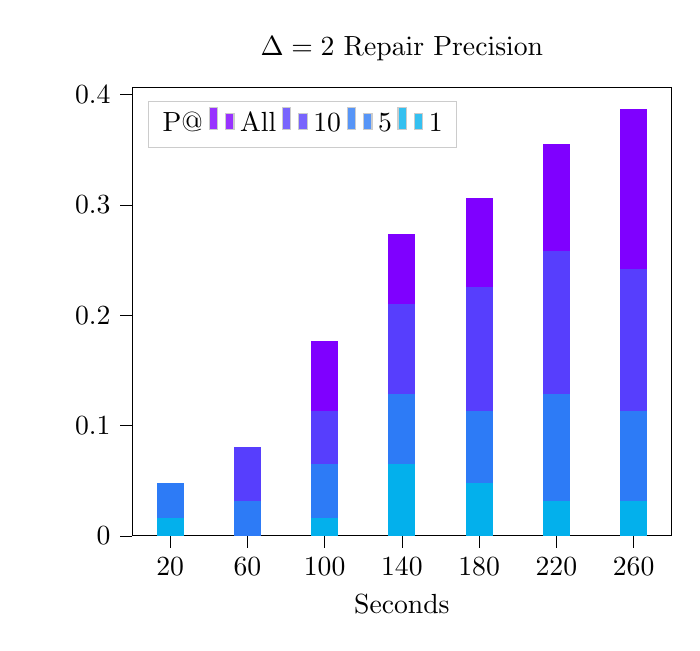
\begin{tikzpicture}

\definecolor{darkgray176}{RGB}{176,176,176}
\definecolor{darkviolet1270255}{RGB}{127,0,255}
\definecolor{deepskyblue3176236}{RGB}{3,176,236}
\definecolor{dodgerblue45123246}{RGB}{45,123,246}
\definecolor{lightgray204}{RGB}{204,204,204}
\definecolor{royalblue8762253}{RGB}{87,62,253}

\begin{axis}[
legend cell align={left},
legend style={fill opacity=0.8, draw opacity=1, text opacity=1, draw=lightgray204, legend columns=-1, legend pos=north west},
tick align=outside,
tick pos=left,
title={$\Delta=2$ Repair Precision},
x grid style={darkgray176},
xlabel={Seconds},
xmin=-0.4925, xmax=6.4925,
xtick style={color=black},
xtick={0,1,2,3,4,5,6},
xticklabels={20,60,100,140,180,220,260},
y grid style={darkgray176},
ylabel={\phantom{Precision@k}},
ymin=0, ymax=0.40635,
ytick style={color=black}
]
\addlegendimage{empty legend}
\addlegendentry{P@}
\draw[draw=none,fill=darkviolet1270255] (axis cs:-0.175,0) rectangle (axis cs:0.175,0.048);
\addlegendimage{ybar,ybar legend,draw=none,fill=darkviolet1270255}
\addlegendentry{All}

\draw[draw=none,fill=darkviolet1270255] (axis cs:0.825,0) rectangle (axis cs:1.175,0.081);
\draw[draw=none,fill=darkviolet1270255] (axis cs:1.825,0) rectangle (axis cs:2.175,0.177);
\draw[draw=none,fill=darkviolet1270255] (axis cs:2.825,0) rectangle (axis cs:3.175,0.274);
\draw[draw=none,fill=darkviolet1270255] (axis cs:3.825,0) rectangle (axis cs:4.175,0.306);
\draw[draw=none,fill=darkviolet1270255] (axis cs:4.825,0) rectangle (axis cs:5.175,0.355);
\draw[draw=none,fill=darkviolet1270255] (axis cs:5.825,0) rectangle (axis cs:6.175,0.387);
\draw[draw=none,fill=royalblue8762253] (axis cs:-0.175,0) rectangle (axis cs:0.175,0.048);
\addlegendimage{ybar,ybar legend,draw=none,fill=royalblue8762253}
\addlegendentry{10}

\draw[draw=none,fill=royalblue8762253] (axis cs:0.825,0) rectangle (axis cs:1.175,0.081);
\draw[draw=none,fill=royalblue8762253] (axis cs:1.825,0) rectangle (axis cs:2.175,0.113);
\draw[draw=none,fill=royalblue8762253] (axis cs:2.825,0) rectangle (axis cs:3.175,0.21);
\draw[draw=none,fill=royalblue8762253] (axis cs:3.825,0) rectangle (axis cs:4.175,0.226);
\draw[draw=none,fill=royalblue8762253] (axis cs:4.825,0) rectangle (axis cs:5.175,0.258);
\draw[draw=none,fill=royalblue8762253] (axis cs:5.825,0) rectangle (axis cs:6.175,0.242);
\draw[draw=none,fill=dodgerblue45123246] (axis cs:-0.175,0) rectangle (axis cs:0.175,0.048);
\addlegendimage{ybar,ybar legend,draw=none,fill=dodgerblue45123246}
\addlegendentry{5}

\draw[draw=none,fill=dodgerblue45123246] (axis cs:0.825,0) rectangle (axis cs:1.175,0.032);
\draw[draw=none,fill=dodgerblue45123246] (axis cs:1.825,0) rectangle (axis cs:2.175,0.065);
\draw[draw=none,fill=dodgerblue45123246] (axis cs:2.825,0) rectangle (axis cs:3.175,0.129);
\draw[draw=none,fill=dodgerblue45123246] (axis cs:3.825,0) rectangle (axis cs:4.175,0.113);
\draw[draw=none,fill=dodgerblue45123246] (axis cs:4.825,0) rectangle (axis cs:5.175,0.129);
\draw[draw=none,fill=dodgerblue45123246] (axis cs:5.825,0) rectangle (axis cs:6.175,0.113);
\draw[draw=none,fill=deepskyblue3176236] (axis cs:-0.175,0) rectangle (axis cs:0.175,0.016);
\addlegendimage{ybar,ybar legend,draw=none,fill=deepskyblue3176236}
\addlegendentry{1}

\draw[draw=none,fill=deepskyblue3176236] (axis cs:0.825,0) rectangle (axis cs:1.175,0);
\draw[draw=none,fill=deepskyblue3176236] (axis cs:1.825,0) rectangle (axis cs:2.175,0.016);
\draw[draw=none,fill=deepskyblue3176236] (axis cs:2.825,0) rectangle (axis cs:3.175,0.065);
\draw[draw=none,fill=deepskyblue3176236] (axis cs:3.825,0) rectangle (axis cs:4.175,0.048);
\draw[draw=none,fill=deepskyblue3176236] (axis cs:4.825,0) rectangle (axis cs:5.175,0.032);
\draw[draw=none,fill=deepskyblue3176236] (axis cs:5.825,0) rectangle (axis cs:6.175,0.032);
\end{axis}

\end{tikzpicture}
}
  \caption{Human repair benchmark. Note the y-axis across different edit distance plots has varying ranges.}\label{fig:human}
\end{figure}